\documentclass[a4paper,12pt, oneside]{mwbk}

\usepackage[utf8]{inputenc}
\usepackage[T1]{polski}
\usepackage{helvet}
\usepackage{graphicx}
\usepackage{color}
\usepackage{geometry}
\usepackage{cite}
\usepackage{url}
\usepackage{setspace}
\usepackage{parskip}
\usepackage{indentfirst}
\usepackage{float}
\usepackage{listings}
\usepackage{wrapfig}
\usepackage[table]{xcolor}
\setlength{\parskip}{2ex}
\setlength{\parindent}{30pt}

%\geometry{hmargin={2cm, 2cm}, height=10.0in}
\geometry{total={210mm,297mm}, left=20mm,right=20mm,bindingoffset=10mm,
top=25mm, bottom=25mm} 

%\includeonly{introduction}

% \makeatletter
% \renewcommand\paragraph{\@startsection{paragraph}{4}{\z@}%
%   {-3.25ex\@plus -1ex \@minus -.2ex}%
%   {1.5ex \@plus .2ex}%
%   {\normalfont\normalsize\bfseries}}
% \makeatother

\sloppy %zakaz wydłużania linii (gdy nie może złożyć) 
\brokenpenalty=10000 %nie dieli wyrazów pomiędzy stronami 
\clubpenalty=10000 %nie pozostawia sierot pojedynczych
\widowpenalty=10000 %nie pozostawia wdów pojedynczych

\begin{document}

\thispagestyle{empty}
%% ------------------------ NAGLOWEK STRONY ---------------------------------

\includegraphics[height=37.5mm]{../images/agh_nzw_a_pl_1w_wbr_rgb_150ppi.jpg}\\
\rule{30mm}{0pt}
{\large \textsf{Wydział Fizyki i Informatyki Stosowanej}}\\
\rule{\textwidth}{3pt}\\
\rule[2ex]
{\textwidth}{1pt}\\
\vspace{7ex}
\begin{center}
{\LARGE \bf \textsf{Praca magisterska}}\\
\vspace{13ex}
% --------------------------- IMIE I NAZWISKO -------------------------------
{\bf \Large \textsf{Łukasz Hanusiak, Mariusz Nowacki}}\\
\vspace{3ex}
{\sf\small kierunek studiów:} {\bf\small \textsf{informatyka stosowana}}\\
\vspace{1.5ex}
{\sf\small specjalność:} {\bf\small \textsf{informatyka w nauce i technice}}\\
\vspace{10ex}
%% ------------------------ TYTUL PRACY --------------------------------------
{\bf \huge \textsf{Rozwój platformy robota mobilnego}}\\
\vspace{14ex}
%% ------------------------ OPIEKUN PRACY ------------------------------------
{\Large Opiekun: \bf \textsf{dr hab. inż. Marek Idzik}}\\
\vspace{22ex}
{\large \bf \textsf{Kraków, kwiecień 2011}}
\end{center}
%% =====  STRONA TYTUŁOWA PRACY MAGISTERSKIEJKIEJ ====

\newpage

%% =====  TYŁ STRONY TYTUŁOWEJ PRACY MAGISTERSKIEJKIEJ ====
{\sf Oświadczam, świadomy(-a) odpowiedzialności karnej za poświadczenie nieprawdy, że niniejszą pracę dyplomową wykonałem(-am) osobiście i samodzielnie i  nie korzystałem(-am) ze źródeł innych niż wymienione w pracy.}

\vspace{14ex}

\begin{center}
\begin{tabular}{lr}
~~~~~~~~~~~~~~~~~~~~~~~~~~~~~~~~~~~~~~~~~~~~~~~~~~~~~~~~~~~~~~~~~ &
................................................................. \\
~ & {\sf (czytelny podpis)}\\
\end{tabular}
\end{center}

%% =====  TYL STRONY TYTULOWEJ PRACY MAGISTERSKIEJKIEJ ====

\newpage
\rightline{Kraków, ?? kwiecień 2011}
\begin{center}
{\bf Tematyka pracy magisterskiej i praktyki dyplomowej
Łukasza Hanusiaka oraz Mariusza Nowackiego
studentów V roku studiów kierunku informatyka stosowana, informatyka w nauce i technice}\\
\end{center}

Temat pracy magisterskiej:
{\bf Rozwój platformy robota mobilnego}\\

\begin{tabular}{rl}

Opiekun pracy:                  & dr hab. inż. Marek Idzik\\
Recenzenci pracy:               & ??? ??? \\
Miejsce praktyki dyplomowej:    & WFiIS AGH, Kraków\\
\end{tabular}

\begin{center}
{\bf Program pracy magisterskiej i praktyki dyplomowej}
\end{center}

\begin{enumerate}
\item Omówienie realizacji pracy magisterskiej z opiekunem.
\item Zebranie i opracowanie literatury dotyczącej tematu pracy.
\item Praktyka dyplomowa:
\begin{itemize}
\item zapoznanie się z ideą...,
\item uczestnictwo w eksperymentach/przygotwanie oprogramowania...,
\item dyskusja i analiza wyników...
\item sporządzenie sprawozdania z praktyki.
\end{itemize}
\item Kontynuacja obliczeń związanych z tematem pracy magisterskiej.
\item Zebranie i opracowanie wyników obliczeń.
\item Analiza wyników obliczeń numerycznych, ich omówienie i zatwierdzenie przez opiekuna.
\item Opracowanie redakcyjne pracy.
\end{enumerate}


\noindent
Termin oddania w dziekanacie: ?? kwiecień 2011\\[1cm]

\begin{center}
\begin{tabular}{lcr}
.............................................................. & ~~~ &
.............................................................. \\
(podpis kierownika katedry) & & (podpis opiekuna) \\
\end{tabular}
\end{center}

\newpage

\noindent
Na kolejnych dwóch stronach proszę dołączyć kolejno recenzje pracy popełnione przez Opiekuna oraz Recenzenta (wydrukowane z systemu MISIO i podpisane przez odpowiednio Opiekuna i Recenzenta pracy). Papierową wersję pracy (zawierającą podpisane recenzje) proszę złożyć w dziekanacie celem rejestracji co najmniej na tydzień przed planowaną obroną.

\linespread{1.3}
\selectfont

\newpage
\tableofcontents

\newpage 
\chapter*{Wprowadzenie}
Celem pracy magisterskiej jest rozwój systemu robota mobilnego
zrealizowanego pierwotnie w pracy magisterskiej pt.: ,,Rozwój systemu sterowania
dla robota mobilnego''\cite{KmakMScThesis2009}. Temat pracy daje dużą swobodę w
wyborze kierunku rozwoju części sprzętowej oraz programowej robota. Niniejsza
praca zajmuje się proces rozbudową robota Dark Explorer, począwszy od analizy
konfiguracji początkowej, poprzez poprawę wydajności istniejących elementów, aż
po dodanie całkiem nowych funkcjonalności. Praca magisterska wymagała wiedzy z
zakresu elektroniki, fizyki oraz szeroko pojętej informatyki.

W ramach pracy magisterskiej zostały podłączone oraz oprogramowane czujniki
składające się na inercjalną jednostkę pomiarową. Jednostka ta umożliwia
rejestrowanie toru ruchu, po którym robot jest przenoszony przez użytkownika.
Podjęto również próbę stworzenia inercjalnego systemu nawigacyjnego w celu
rozwiązania problemu rekonstrukcji ścieżki powrotnej na podstawie danych
zarejestrowanych przy pomocy czujnika przyspieszenia oraz żyroskopu. W trakcie
odtwarzania powrotnego toru ruchu robot, wykorzystując dane z dołączonych do
niego dalmierzy, jest w stanie uniknąć zderzenia z napotkanymi przeszkodami
jednocześnie starając się dotrzeć do punktu startowego. W pracy magisterskiej
zawarty jest również przewodnik pozwalający programistom, nie posiadającym
doświadczenia w tworzeniu oprogramowania dla systemów wbudowanych, zaznajomić się
z narzędziami pomocnymi w rozwoju programów sterujących mikrokontrolerami
opartymi o architekturę ARM. Poruszono także tematykę rozwoju aplikacji
sterujących robotem dedykowanych na urządzenia mobilne oraz stacjonarne. Efektem
tego jest stworzone oprogramowanie działające na komputerach oraz telefonach z
obsługą technologii Java ME oraz .NET. Podczas tworzenia oprogramowania położono
szczególny nacisk na przenośność wszystkich rozwiązań na różne środowiska
uruchomieniowe oraz intuicyjną obsługę i prostą rozbudowę oprogramowania.

W rozdziale pierwszym przedstawiono dzieje robotyki od jej początków, aż po dzień
dzisiejszy. W ramach tego rozdziału, zaprezentowane zostały dziedziny w jakich
współcześnie roboty znajdują zastosowanie. Nie zabrakło również podstawowych
informacji na temat sposobów klasyfikacji i podziału robotów. Rozdział ten ma na
celu wprowadzenie użytkownika w zagadnienia z którymi robotyka zmaga się na co
dzień.

Rozdział drugi przedstawia analizę sprzętu oraz oprogramowania robota Dark
Explorer stworzonych w ramach poprzedniej pracy magisterskiej. Zwraca on uwagę na
możliwości oraz potencjalne przeszkody które mogą się pojawić podczas rozwoju
robota.

Trzeci rozdział opisuje narzędzia, oraz sposób ich konfiguracji, niezbędne
podczas rozwoju oprogramowania dla systemów wbudowanych. Ze względu na znaczące
różnice pomiędzy narzędziami przeznaczonymi dla systemu Windows i Linux, zostały
one omówione w ramach oddzielnych podrozdziałów.

W rozdziale czwartym poruszana jest tematyka związana z tworzeniem oprogramowania
sterującego robotem działającego na urządzeniach mobilnych oraz stacjonarnych.

Rozdział piąty przedstawia rozszerzenia warstwy sprzętowej wprowadzone w trakcie
realizacji pracy magisterskiej. Czytelnik znajdzie tutaj szczegółowy opis zasady
działania i możliwych zastosowań dla czujników dołączonych do nowej wersji robota
Dark Explorer. W ramach rozdziału omówiono również sposób konstrukcji obudowy
pozwalającej na wygodne podłączanie wszystkich elementów rozszerzających
dotychczasowe możliwości robota.

Szósty rozdział prezentuje funkcje oprogramowania systemu wbudowanego
rozwiązujące problemy takie jak: rekonstrukcja ścieżki powrotnej, omijanie
przeszkód, pobieranie obrazu z kamery z maksymalną dostępną rozdzielczością oraz
detekcja twarzy na obrazie statycznym. Opisany jest również protokół komunikacji
bluetooth warstwy aplikacji modelu referencyjnego ISO.

Złożoność problemów realizowanych w ramach tej pracy magisterskiej oraz szeroki
zakres wiedzy konieczny do jej realizacji wymagał aby była ona realizowana w
zespole dwuosobowym.
\section{Historia i rozwój robotyki}
Robotyka jest stosunkowo młodą dziedziną nauki łączącą różne gałęzie nauk
technicznych i nie tylko. Do pełnego zrozumienia zagadnień współczesnej robotyki
oraz budowy i zastosowań robotów konieczna jest niejednokrotnie rozległa wiedza
na temat elektroniki, mechaniki, inżynierii przemysłowej, matematyki oraz
szeroko pojętej informatyki. Ponadto wiele nowopowstałych gałęzi wiedzy
zajmujących się rozwojem sztucznej inteligencji, modelowaniem sztucznego życia czy rozwojem
inżynierii wiedzy coraz częściej staje się nierozerwalnie związane z problemami
współczesnej robotyki. Nie należy zapominać również o tym, że rozwój inżynierii
wytwarzania oraz automatyki przemysłowej pozwala na nieustanny rozwój robotyki z
którą mamy do czynienia w przemyśle w dniu dzisiejszym.\\
\\
Pojęcie ``Robot'' w literaturze pojawił się po raz pierwszy w sztuce czeskiego
pisarza Karel'a Capka w roku 1920. Termin ``robot'' oznacza w języku czeskim
pracę lub służbę przymusową. Nieco ponad 20 lat później, amerykański uczony i
pisarz Isaac Assimov w jednym ze swoich opowiadań po raz pierwszy używa słowa
robotyka. W kolejnych latach Assimov w swojej twórczości niejednokrotnie wraca
do problemu robotyki skutkiem czego jest wydanie w 1950 roku zbioru opowiadań
pod tytułem ``Ja, robot''. Jako ciekawostkę można dodać, że w wydanym w 1942
roku opowiadaniu pod tytułem ``Zabawa w berka'', Assimove wprowadza trzy prawa
robotyki, według których zdaniem autora powinny być programowane roboty.
\begin{description}
\item[Prawo pierwsze] \hfill \\
Robot nie może zranić istoty ludzkiej, ani przez zaniedbanie narazić człowieka
na zranienie. 
\item[Prawo drugie] \hfill \\
Robot musi spełniać polecenia wydawane przez człowieka, poza poleceniami
sprzecznymi z prawem pierwszym.
\item[Prawo trzecie] \hfill \\
Robot musi chronić samego siebie dopóki nie jest to sprzeczne z prawami
pierwszym i drugim.
\end{description} 
Nieco później, Isaac Assimov, jako uzupełnienie i prawo nadrzędne dodaje prawo
zerowe o następującym brzmieniu ``Robot nie może szkodzić ludzkości, ani przez zaniedbanie narazić ludzkości na
szkodę''. Oprócz wspomnianych powyżej podstawowych praw, zdefiniowano również
inne prawa wynikające z prowadzonych badań w tej dziedzinie i rozwoju robotyki.\\
\\
Dzięki gwałtownemu rozwojowi techniki w czasie II wojny światowej w roku 1956
GC. Devol i JF. Engelberger zainspirowani twórczością Assimov'a zaprojektowali i
stworzyli pierwszy w dziejach ludzkości działający egzemplarz robota.
Engelberger założył firmę pod nazwą ``Unimation'' zajmującą się automatyzacją,
pierwszym robotem stworzonym przez firmę Engelbergera był robot nazwany
``Unimate''. Został on zainstalowany w fabryce General Motors w Trenton gdzie
został przystosowany do obsługi wysokociśnieniowej maszyny odlewniczej. W
kolejnych latach roboty firmy ``Unimation'' znalazły swoje zastosowanie w innych
gałęziach przemysłu, a sam Engelberger otrzymał miano ojca robotyki.\\
\\
Nieco później, bo w roku 1979 Robotics Industries Association 
zdefiniowało robota jako wielofunkcyjny, programowalny manipulator
zaprojektowany do przenoszenia materiałów, narzędzi, części urządzeń poprzez
serię programowalnych ruchów wykonywanych w celu realizacji różnych zadań.
W myśl wspomnianej definicji jedną z podstawowych cech robota jest jego
progrmowalność i możliwość dostosowywania się do zmiennych warunków środowiska
pracy. \\
Pierwsze roboty projektowano z myślą o zastosowaniu ich do realizacji
elementarnych zadań związanych z przenoszeniem elementów z jednego punktu do
drugiego. Program pracy robota miał więc charakter sekewencji operacji
prowadzących do realizacji określonego przez programistę zadania. W miarę
rozwoju technicznego, stawiane przed robotami zadania wymusiły użycie przez
konstruktorów czujników które pozwalały na zwiększenie poziomu interakcji
robotów z otoczeniem, a co za tym idzie umożliwiły realizowanie zadań o wysokim
stopniu złożoności. Od tego momentu kierunek rozwoju robotyki obrał
sobie za cel stworzenie maszyny na tyle uniwersalnej i niezależnej aby mogła
nosić miano androida. Jednak do realizacji tego zadania konieczne jest
opracowanie sztucznej inteligencji na którą z pewnością przyjdzie nam jeszcze
trochę poczekać. \\
\\
Pierwszym krokiem na drodze do stworzenia androida było oderwanie robota od
stałego miejsca instalacji i pozwolenie mu w miarę możliwości swobodne
poruszanie się dostępnej mu przestrzeni roboczej. Tak powstała klasa robotów
które mogą przemieszczać się za pomocą kół, gąsienic czy nawet kończyn lub
odnóży. Roboty tego typu potrafią pływać, latać i sprawnie poruszać się
po lądzie dodatkowym ich atutem jest fakt iż większość z nich posiada niemal
całkowitą autonomię i ograniczona jest jedynie poprzez wielkość otoczenia w
jakim zostały umieszczone. Takim sposobem roboty powstała grupa robotów
nazywanych robotami mobilnymi. Cechą wspólną wszystkich urządzeń z tej rodziny
była umiejętność swobodnego przemieszczania się oraz analiza najbliższego
otoczenia. Na tej podstawie maszyna mogła przeprowadzić wnioskowanie pozwalające
na podejmowanie dalszych akcji czy też zakomunikowanie użytkownikowi odczytanych
parametrów środowiska.\newpage
Historię robotów mobilny zapoczątkował amerykański Uniwersytet w Stanford gdyż
w roku 1968 jako pierwszy stworzył w pełni działający model robota mobilnego pod
nazwą Shakey. Nazwa została zainspirowana szarpanymi ruchami z jakimi robot się
poruszał. Głównym zadaniem robota było modelowanie otoczenia w którym się
znajdował. W ślad za Uniwersytetem w Stanford ruszyło MIT. W roku 1983 posiadali
już pierwszy działający model robota swobodnie skaczącego. Niecałe 6
lat później MIT stworzyło pierwszego robota kroczącego wzorowanego na owadach.
Robot ten sterowany był za pomocą wielowarstwowych automatów o stanach
skończonych, a ze światem zewnętrznym komunikował się za pomocą czułek,
inklinometrów, czujników zbliżeniowych na podczerwień. Genghis, bo tak
nazwany został robot, posiadał na pokładzie 4 ośmiobitowe jednostki obliczeniowe, ważył
niecały kilogram i miał 35 cm długości.

\begin{figure}[hb]
 \centering
 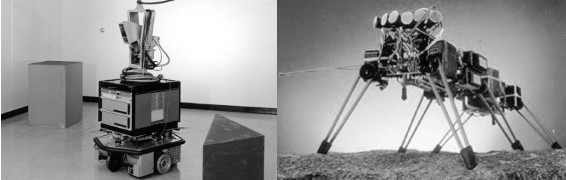
\includegraphics[height=50mm]{../images/ch01/shakey_and_genghis.png}
 \caption{Od lewej: Shakey (Stanford), Genghis (MIT) }
 \label{fig:RobotsHistory_Shakey_Genghis}
\end{figure}

Po sukcesie wspomnianych projektów,
rozwój robotów mobilnych następował już bardzo dynamiczne. W latach 90
powstawało wiele różnych modeli robotów o bardzo różnorodnych rodzajach napędów
oraz zestawach czujników umożliwiających interakcje ze światem zewnętrznym.

\begin{figure}[hb]
 \centering
 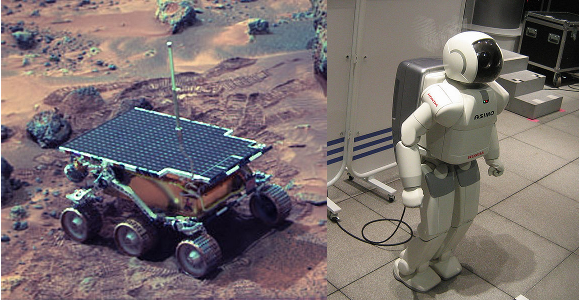
\includegraphics[height=60mm]{../images/ch01/pathfinder_and_asimo.png}
 \caption{Kolejno: Pathfinder (NASA), Asimo (Honda)}
 \label{fig:RobotsHistory_Pathfinder_Asimo}
\end{figure}

Swoistym ukoronowaniem prac było w 1997 roku stworzenie przez NASA robota o
nazwie Pathfinder. Robot wyposażony był w czujniki laserowe, stereowizję,
żyroskopy i inne rodzaje czujników o charakterze badawczym. Zasilany był on
bateriami słonecznymi które pozwoliły mu na 83 dni nieprzerwanej pracy podczas
której robot przebyło około 100 metrów i wykonał 230 manewrów. W ostatnich
latach do największych osiągnięć robotyki mobilnej można z pewnością zaliczyć
powstanie robotów humanoidalnych takich jak japoński ASIMO. Robot ten ważył 54
kg i posiadał 130 cm wysokości. Wersja z roku 2005 potrafiła biegnąc osiągnąć
prędkość dochodzącą nawet do do 6 km/h. Ponad to robot potrafił wchodzić w
interakcję z otoczającymi go ludźmi i przedmiotami. Urządzenie stworzone przez
inżynierów z firmy Honda potrafiło rozpoznawać gesty takie jak podanie ręki,
wskazanie kierunku czy machanie ręką na porzegnanie. Robot równie dobrze radził
sobie z rozpoznawaniem twarzy, dźwięków i analizą otaczającego go środowiska.
Potrafił on rozpoznać i omijać niebezpieczeństwa postawione na jego drodze jak
na przykład schody czy osoby poruszające się w jego kierunku.\\
\\
Obserwując postęp w dziedzinie robotyki można odnieść wrażenie iż w dzisiejszych
czasach roboty znalazły dla siebie zastosowanie niemal w każdej dziedzinie
życia. Od wielu lat sprawdzają się już w przemyśle, transporcie, budownictwie
oraz są niezastąpione w środowiskach nieprzyjaznych człowiekowi, takich jak
podmorskie głębiny czy otchłań kosmosu. Obszar zastosowań robotów jest
tak szeroki iż wydawać się może, że jedynym czynnikiem ograniczającym rozwój
współczesnej robotyki są względy czysto ekonomiczne. Nie staje to jednak na
przeszkodzie do projektowania i tworzenia przez konstruktorów z całego świata
rozwiązań powoli przybliżających ludzkość do stworzenia w pełni samodzielnego
oraz inteligentnego androida.


\newpage
\chapter{Dark Explorer pod lupą}
\begin{figure}[!ht]
 \centering
 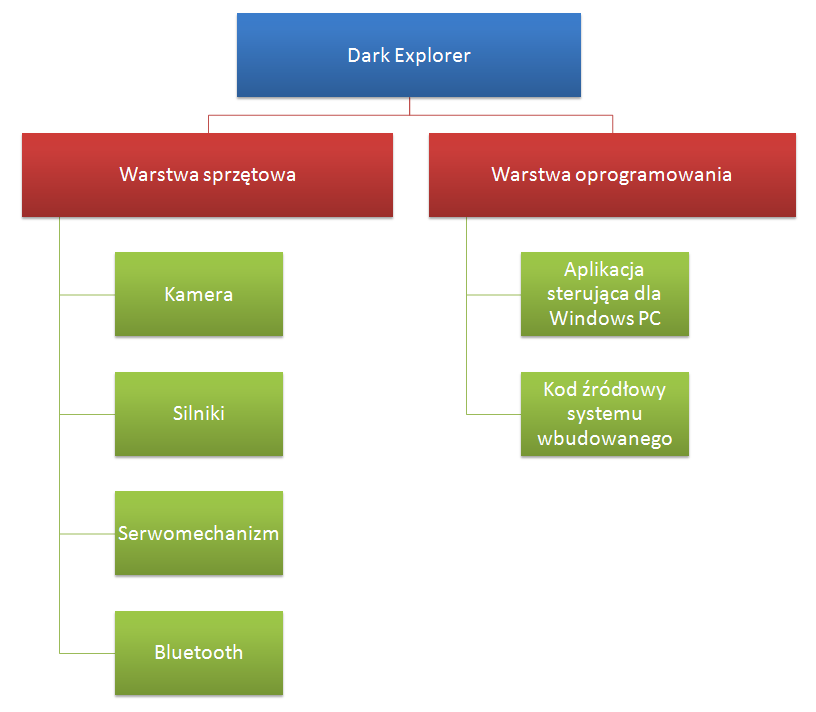
\includegraphics[height=125mm]{../images/ch02/kmak_platform.png}
 \caption{Struktura platformy robota mobilnego zreazlizowanej w ramach
 poprzedniej pracy magisterskiej\cite{KmakMScThesis2009}}
 \label{fig:KmakPlatform}
\end{figure}
%W tym rozdziale zostanie opisana konfiguracja pierwotna robota z wyszczególnieniem elementów, które mogą być problemem przy dalszym rozwoju możliwości tego urządzenia.
\begin{figure}[!ht]
 \centering
 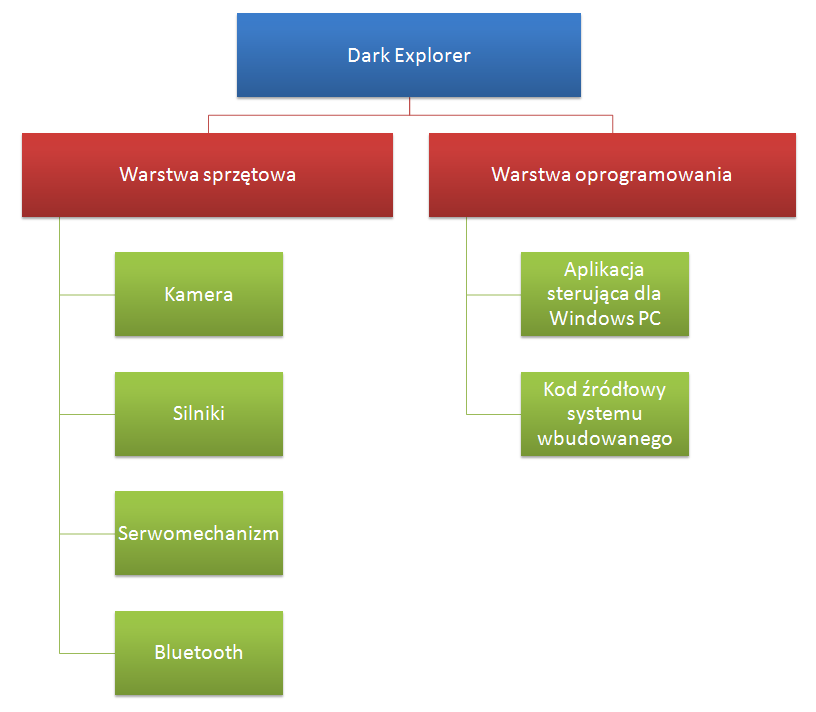
\includegraphics[height=125mm]{../images/ch02/kmak_platform.png}
 \caption{Struktura platformy robota mobilnego zrealizowanej w ramach
 poprzedniej pracy magisterskiej\cite{KmakMScThesis2009}}
 \label{fig:KmakPlatform}
\end{figure}

\section{Analiza sprzętu}
Dark Explorer jest autonomicznym robotem mobilnym z wbudowaną kolorową kamerą cyfrową VGA. Jego podstawowe możliwości to:
\begin{itemize}
 \item jazda ze zmienną prędkością w przód, tył, lewo oraz prawo
 \item komunikacja z urządzeniami zewnętrznymi przy pomocy technologii bluetooth
 \item wykonywanie zdjęć z maksymalną rozdzielczością $160x100$ pikseli w kolorze oraz $320x200$ pikseli w odcieniach szarości
 \item poruszanie wieżyczką na której zainstalowana jest kamera
 \item wykrywanie prostych wzorców przy pomocy analizy obrazu oraz podążanie za nimi
\end{itemize}

\subsection{Elementy elektroniczne}
Dark Explorer został wyposażony w mikrokontroler zarządzający AT91Sam7s256 o częstotliwości pracy zegara maksymalnie do 50 MHz oraz wbudowanej szybkiej pamięci SRAM 64 kB. Mikrokontroler ten jest bogaty w różnego rodzaju urządzenia peryferyjne takie jak na przykład: TWI\footnote{TWI -- Two Wire Interfece znany również jako $I^{2}C$, interfejs szeregowej komunikacji danych}, RTT\footnote{RTT -- Real Time Timer, służy do odmierzania dłuższych odcinków czasu}, PDC\footnote{PDC -- Peripheral DMA Controller, kontroler DMA}, AIC\footnote{AIC -- Advanced Interrupt Controller, kontroler przerywań}, PWM\footnote{PWM -- Pulse Width Modulation Controller}, ADC\footnote{ADC -- Analog to Digital Converter, konwerter analogowo cyfrowy}. To tylko część z nich. Dzięki tak wielkiemu wyborowi urządzeń peryferyjnych mikrokontroler ten daje nam duże możliwości rozwoju konfiguracji. Częstotliwość pracy mikrokontrolera ARM7 jest wystarczająca do zadań przez niego wykonywanych.

Większość elementów elektronicznych robota jest umieszczonych na płycie głównej zaprojektowanej przez autora projektu robota. Jest ona bardzo dobrze przemyślana ponieważ pozwala na wykorzystywanie urządzeń peryferyjnych mikrokontolera w praktycznie dowolny sposób. Większość wyjść oraz wejść mikrokontrolera nie jest połączona na stałe z konkretnymi podzespołami Dark Explorera lecz poprzez zworki, które pozwalają podłączanie i odłączanie poszczególnych urządzeń.

\begin{figure}[!ht]
 \centering
 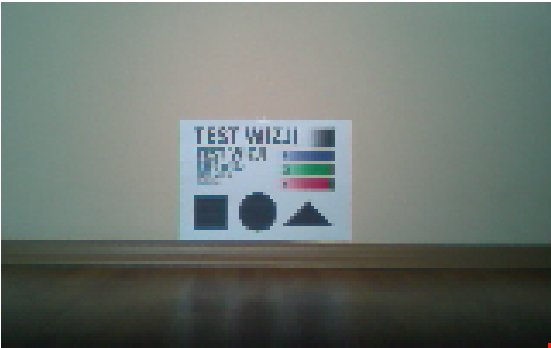
\includegraphics[height=50mm]{../images/ch02/160x100C.jpg}
 \caption{Obraz wykonany przy pomocy kamery zamontowanej w robocie. 160 x 100 pikseli w kolorze. \cite{KmakMScThesis2009}}
 \label{fig:160x100C}
\end{figure}

Twórca Dark Explorera wyposażył go kamerę cyfrową o maksymalnej rozdzielczości $640x480$ pikseli. Jest to urządzenie $PO6040$ firmy Pixelplus. Można go konfigurować przy pomocy interfejsu $I^{2}C$. W konfiguracji pierwotnej robot potrafi odbierać zdjęcia o maksymalnej rozdzielczości $320x200$ pikseli w odcieniach szarości(rys. \ref{fig:320x200BW}) oraz $160x100$ pikseli w kolorze (rys. \ref{fig:160x100C}). Tak niskie rozdzielczości nie są wystarczające do wykrywania i tym bardziej rozpoznawania twarzy na obrazie dlatego też konieczna jest poprawa tych parametrów.

W skład robota wchodzą także silniki napędowe, serwomechanizm, dioda mocy oraz moduł bluetooth. Wszystkie te elementy muszą być podłączone do mikrokontrolera przez konkretne wejścia/wyjścia. Z tego powodu do dyspozycji osób przeprowadzających dalszy rozwój robota pozostało jedynie pięć wejść/wyjść cyfrowych oraz trzy wejścia analogowe. Jest to kolejna przeszkoda którą trzeba będzie pokonać.

\begin{figure}[!ht]
 \centering
 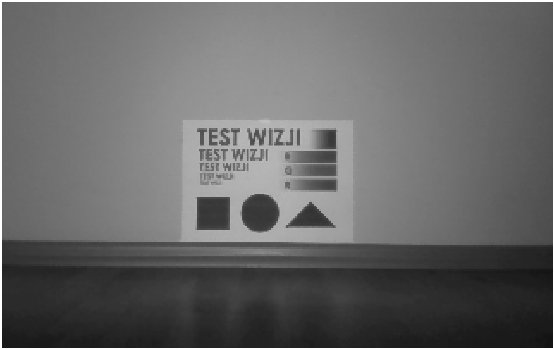
\includegraphics[height=50mm]{../images/ch02/320x200B&W.jpg}
 \caption{Obraz wykonany przy pomocy kamery zamontowanej w robocie. 320 x 200 pikseli w odcieniach szarości \cite{KmakMScThesis2009}}
 \label{fig:320x200BW}
\end{figure}

Robot mobilny komunikuje się z urządzeniami zewnętrznymi przy pomocy modułu bluetooth BTM-222 firmy Rayson. Maksymalna przepustowość danych z jaką potrafi działać wynosi 3Mb/s. Obsługiwane przez niego interfejsy to: USB, UART oraz PCM. Mikrokontroler komunikuje się z modułem bluetooth przy pomocy interfejsu UART o maksymalnej przepustowości 460,8 kb/s. Jak widać takie rozwiązanie nie wykorzystuje pełnych możliwości modułu BTM-222. Bardziej efektywne byłoby skorzystanie z interfejsu USB który potrafi przesyłać dane z prędkością maksymalną od 1,5Mb/s w standardzie USB 1.0 do 5Gb/s w standardzie USB 3.0. Aby dokonać zmiany interfejsu komunikacyjnego pomiędzy mikrokontrolerem a modułem bluetooth konieczna jest ingerencja w konstrukcję płyty głównej robota, gdyż BTM-222 jest przylutowany bezpośrednio do niej \ref{fig:BTM222}.

\begin{figure}[!ht]
 \centering
 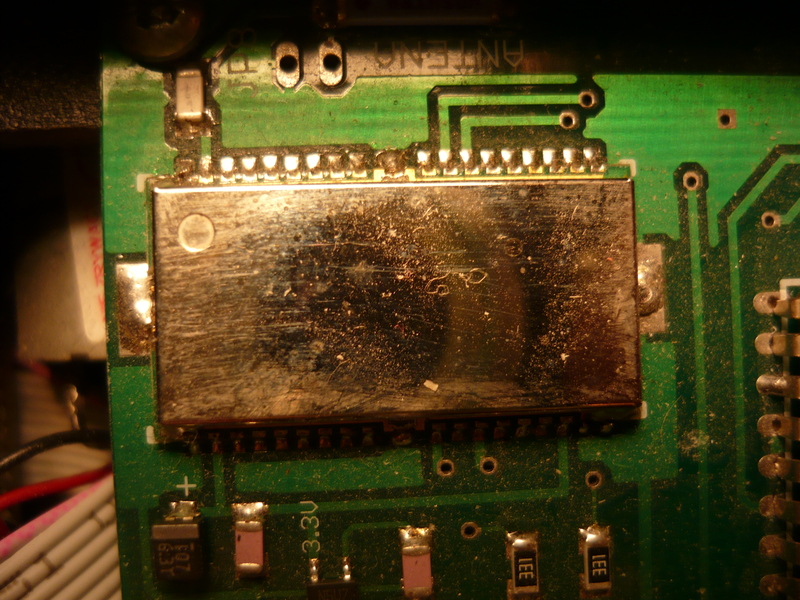
\includegraphics[height=50mm]{../images/ch02/btm-222.jpg}
 \caption{Zdjęcie modułu bluetooth zamontowanego na płycie głównej robota.}
 \label{fig:BTM222}
\end{figure}

\subsection{Elementy mechaniczne}
Konstrukcja obudowy Dark Explorera została wykonana z tworzywa sztucznego i jest dopasowana do elementów które zostały zaprojektowane przez autora. Wewnątrz obudowy nie ma miejsca na jakiekolwiek nowe podzespoły, dlatego też konieczna będzie jej modyfikacja (rys. \ref{fig:KmakMainBoard}).

\begin{figure}[!ht]
 \centering
 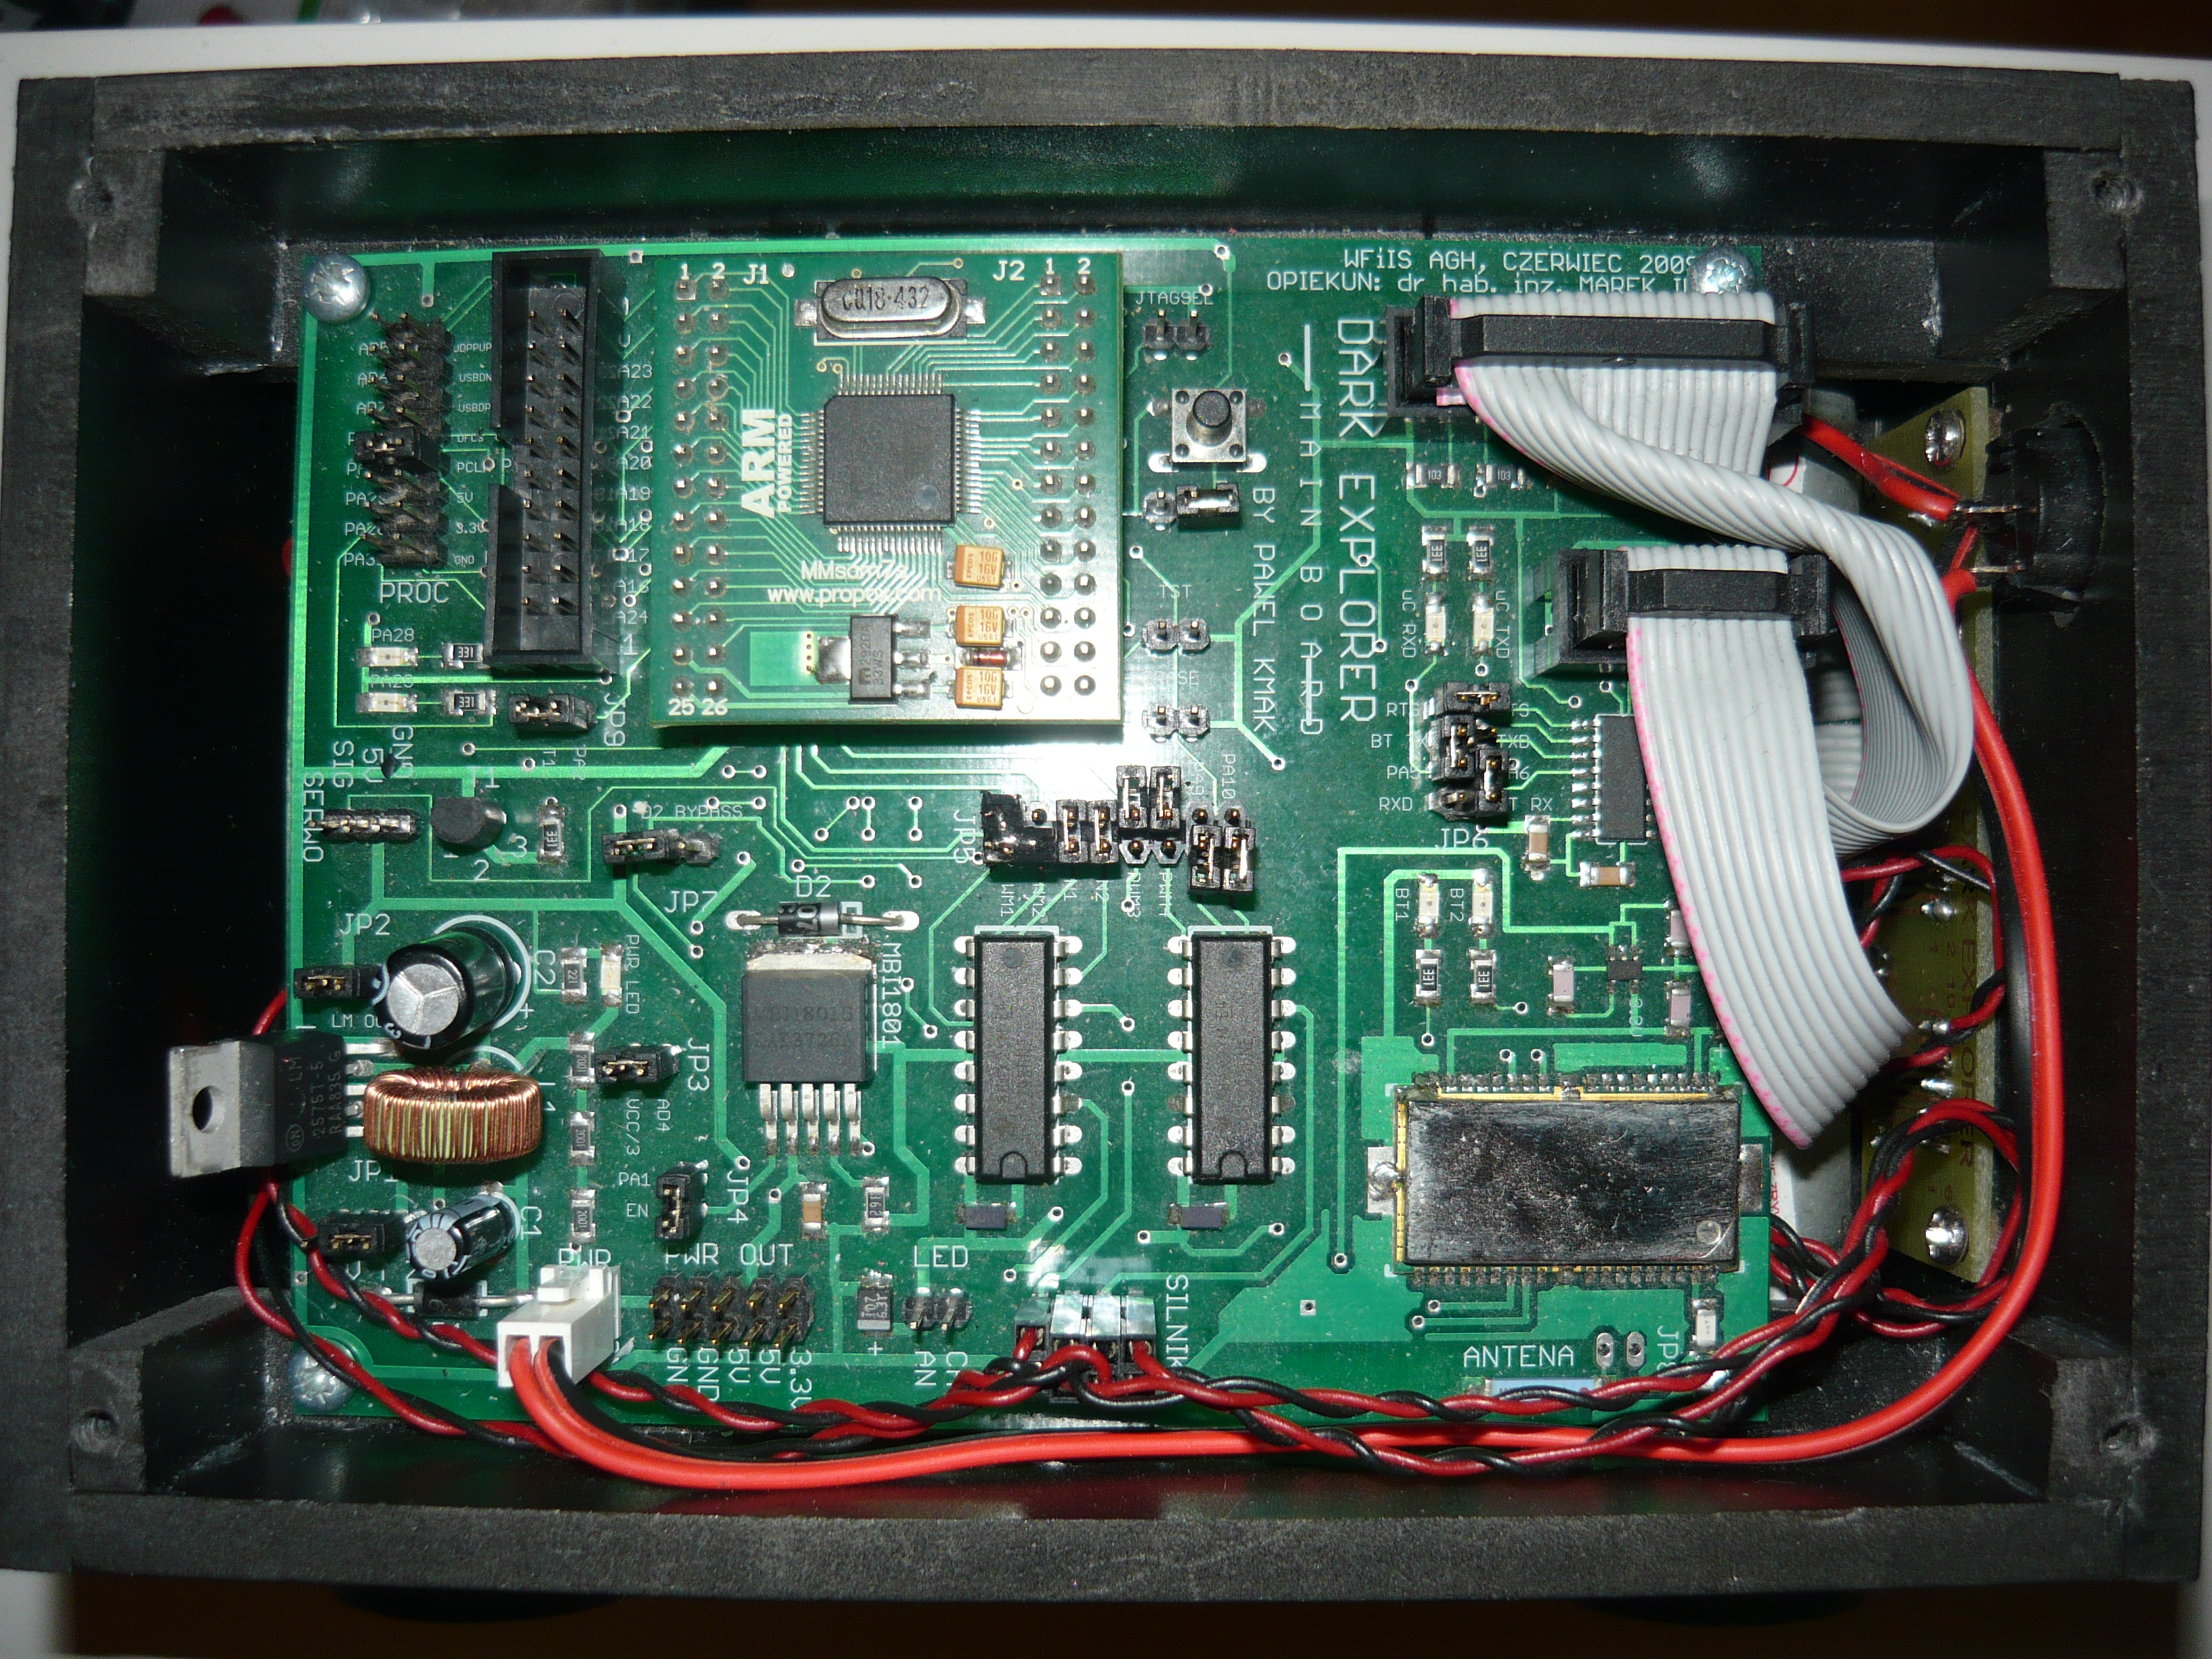
\includegraphics[height=75mm]{../images/ch02/main_board.jpg}
 \caption{Widok na płytę główną Dark Explorer'a}
 \label{fig:KmakMainBoard}
\end{figure}

Podczas testów konfiguracji pierwotnej zauważono lekkie kłopoty robota z poruszaniem się po gładkich powierzchniach. Najprawdopodobniej jest to spowodowane kółkami (rys. \ref{fig:KmakWheel}) zamontowanymi przy robocie, które tracą przyczepność na nieco bardziej śliskim podłożu. Możliwe, że podczas rozwoju robota, konieczna będzie ich wymiana w celu zapewnienia dobrej przyczepności i poprawnego toru jazdy urządzenia.

\begin{figure}[!ht]
 \centering
 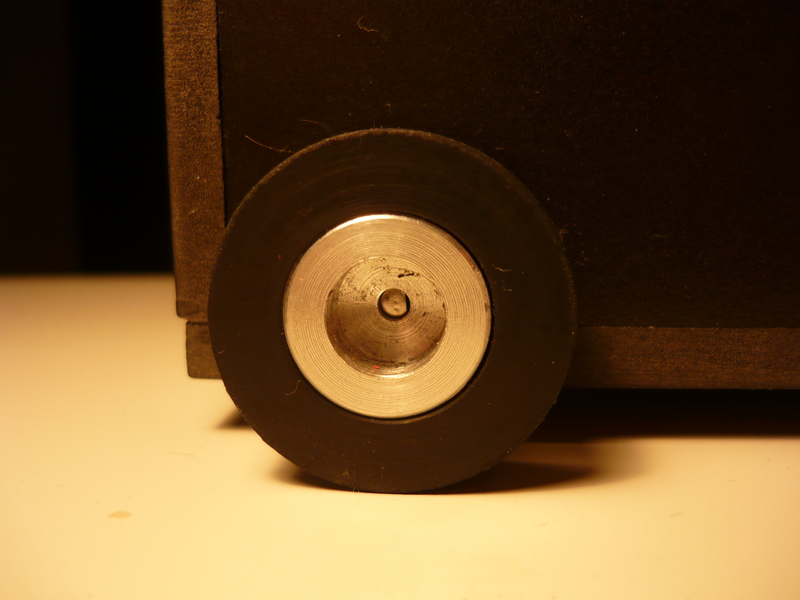
\includegraphics[height=75mm]{../images/ch02/wheel.jpg}
 \caption{Koło napędowe Dark Explorer'a}
 \label{fig:KmakWheel}
\end{figure}

%\chapter{Analiza istniejącej platformy software'owej}
\section{Analiza oprogramowania robota - firmware}
\section{Analiza programu sterującego}


\newpage
\chapter{Rozwój platformy robota mobilnego}
\begin{figure}[!ht]
 \centering
 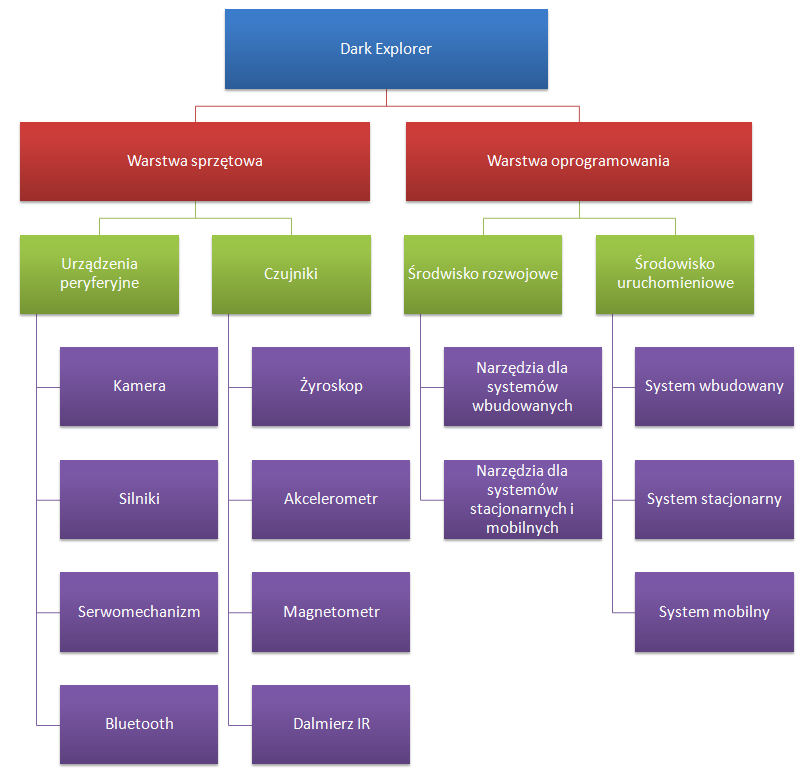
\includegraphics[height=150mm]{../images/ch03/darkexplorer_platform.png}
 \caption{Struktura platformy robota mobilnego po zakończeniu prac}
 \label{fig:DarkExplorerPlatform}
\end{figure}

\newpage
\chapter{Środowisko rozwojowe systemu wbudowanego}
Podczas przygotowywania się do rozpoczęcia pracy z nową technologią, każdy
programista powinien być świadomy tego jakie są istniejące narzędzia, które mogą
mu pomóc w pracy. W tym rozdziale opisany jest sposób instalacji oraz używania
narzędzi wykorzystywanych przez autorów tej pracy.

\begin{figure}[!ht]
 \centering
 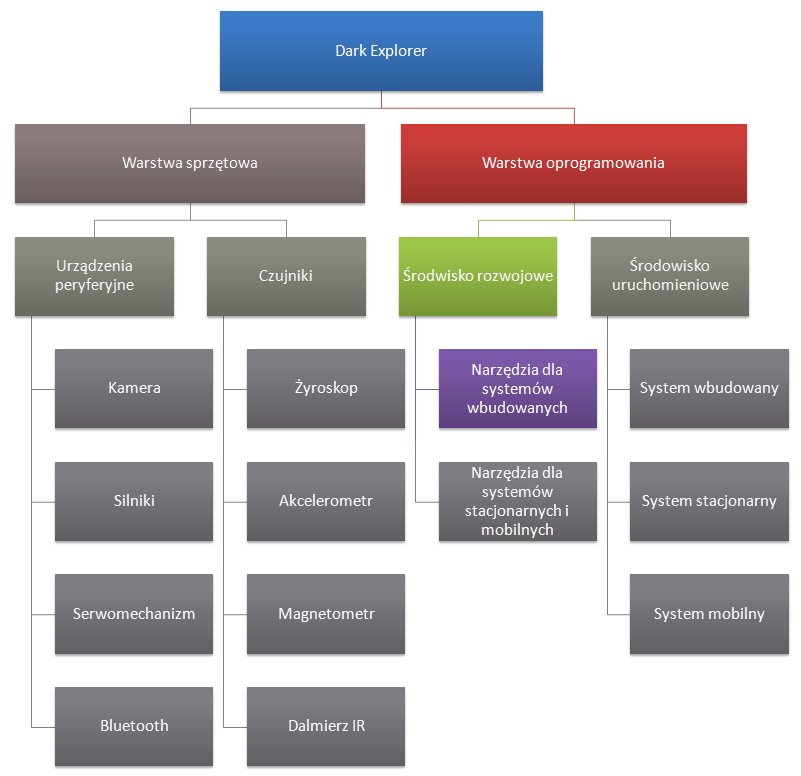
\includegraphics[height=125mm]{../images/ch03/dark_explorer_platform_ide_embeded.png}
 \caption{Struktura platformy robota mobilnego po zakończeniu prac. Kolorem oznaczono zakres prac opisanych w bierzącym rozdziale.}
 \label{fig:DarkExplorerPlatformIDE}
\end{figure}

\section{Narzędzia dla systemu Windows}
\label{sec:embeded-win-tools}
Pierwszym krokiem do przygotowania środowiska rozwojowego umożliwiającego
rozwijanie oprogramowania sterującego robotem jest instalacja sterowników
wymaganych przez system Windows do obsługi interfejsu JTAG\footnote{Joint Test
Action Group - jest to nazwa standardu który definuje protokół wykorzystywany do
testowania połączeń na płytkach drukowanych oraz uruchamiania i programowania
układów i systemów mikroprocesorowych. } za pomocą którego odbywa się proces
wgrywania przygotowanego oprogramowania do pamięci robota. Kolejnym wymaganym
krokiem jest instalacja i konfiguracja narzędzi umożliwiających stworzenie pliku
binarnego umożliwiającego uruchomienie przygotowanej na platformie sprzętowej
robota. Ostatnim etapem przygotowań jest instalacja oprogramowania
umożliwiającego programowanie układu za pomocą wspomnianego interfejsu JTAG oraz
debugowanie aplikacji w trakcie jej działania na robocie.

\subsection{Instalacja WinARM}
Do kompilacji kodu źródłowego oprogramowania zajmującego się sterowaniem
podzespołami robota wykorzystany został zestaw narzędzi znany pod nazwą WinARM.
WinARM jest zestawem narzędzi umożliwiających tworzenie oprogramowania dla
kontrolerów opartych na platformie ARM. W odróżnieniu od innych dostępnych
obecnie rozwiązań, środowisko to, nie wymaga dodatkowej instalacji narzędzi
udostępnianych w ramach MinGW\footnote{Minimalist GNU for Windows - port GCC
dostarczający zestaw darmowych narzędzi do komiplacji natywnych plików
wykonywalnych dla platformy Windows} czy też Cygwina\footnote{Cygwin -
implementacja standardu POSIX przeznaczona dla systemów z rodziny Windows}.
Wszystkie potrzebne narzędzia dostarczane są w ramach SDK\footnote{SDK (z ang.
Software Development Kit) - Zestaw narzędzi do rozwoju oprogramowania}. Narzędzia
WinARM pomyślnie przeszły testy z kontrolerami Atmel AT91SAM7S64, AT91SAM7S256,
AT91RM9200 ARM7TDMI oraz Philips LPC2106, Philips LPC2129, Philips LPC2138,
Philips LPC2148. Dodatkowo dostarczane w ramach środowiska kompilatory i
narzędzia powinny prawidłowo współpracować ze wszystkimi mikrokontrolerami
opartymi o architekturę ARM(-TDMI/Thumb itp.).

Instalację środowiska WinARM należy rozpocząć od pobrania archiwum z najnowszą
wersją narzędzi ze strony
\url{http://gandalf.arubi.uni-kl.de/avr_projects/arm_projects/}. W chwili pisania
pracy dostępna była wersja środowiska WinARM w wersji 20060606. Po zakończeniu
procesu pobierania, archiwum należy rozpakować w taki sposób aby wszystkie
podstawowe narzędzia dostępne były w katalogu \url{C:\WinARM\bin}. Umieszczenie
katalogu z narzędziami WinARM w innej lokalizacji jest również możliwe, ale może
wymagać wykonania dodatkowych operacji konfiguracyjnych w celu zapewnienia
poprawności działania wszystkich narzędzi. Aby udostępnić narzędzia WinARM z
linii poleceń systemu Windows konieczne jest dodanie do zmiennej systemowej
\url{PATH} ścieżki do katalogów z plikami wykonywalnymi biblioteki. W przypadku
instalacji w podanym powyżej katalogu wartości powinny być następujące
\url{C:\WinARM\bin;C:\WinARM\utils\bin;}. Jeżeli jednak katalog z pakietem
został umieszczony w innej lokalizacji konieczne jest odpowiednie zmodyfikowanie
wspomnianych wpisów. Szczegóły okna konfiguracji widoczne są na rysunku
\ref{fig:winarm-config}

\begin{figure}[h!]
 \centering
 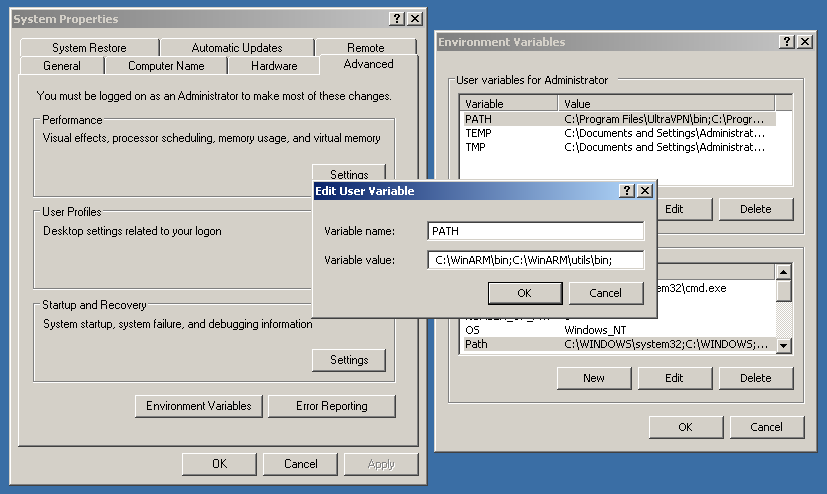
\includegraphics[width=0.95\textwidth]{../images/ch03/winarm-config-win32.png}
 \caption{Konfiguracja narzędzi pakietu WinARM}
 \label{fig:winarm-config}
\end{figure}

\subsection{Instalacja sterowników programatora}
Programowanie oraz debugowanie aplikacji robota może zostać zrealizowane za
pomocą dowolnego programatora kompatybilnego z interfejsem JTAG. Programatory
oparte o interfejs LPT nie wymagają od użytkownika żadnej dodatkowej
konfiguracji. Nieco inaczej wygląda sytuacja z programatorami opartymi o
interfejs USB, które to wymagają przed pierwszym użyciem zainstalowania
sterowników umożliwiających prawidłowe rozpoznanie programatora przez system
Windows. Jednym z bardziej popularnych programatorów USB jest TriTon JTAG. TriTon
JTAG to programator przeznaczony dla procesorów zbudowanych w oparciu o rdzeń ARM
podłączany do komputera za pomocą portu USB. TriTon JTAG posiada standardowe 20
pinowe złącze JTAG wraz z wyprowadzeniami sygnałów RxD i TxD interfejsu UART.
TriTon JTAG współpracuje z OpenOCD, pozwalając na programowanie oraz debugowanie
działającej na urządzeniu aplikacji. Urządzenie oparte jest o układ FT2232 który
umożliwia jego współprace także z innymi środowiskami rozwoju oprogramowania dla
platformy ARM kompatybilnymi z FT2232.

\begin{figure}[h!]
 \centering
 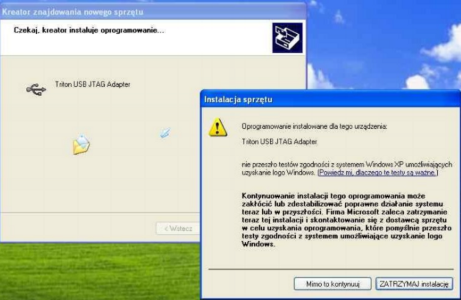
\includegraphics[width=0.85\textwidth]{../images/ch03/jtag-install-s2.png}
 \caption{Instalacja sterowników do programatora TriTon JTAG}
 \label{fig:TritonInstall}
\end{figure}

Instalację programatora należy rozpocząć od pobrania sterowników do układu FT2232
ze strony \url{http://www.ethernut.de/en/download/}. Na stronie dostępne są
sterowniki przeznaczone dla systemów Windows 2000, XP, Server 2003, Vista oraz
Server 2008. Po rozpakowaniu archiwum ze sterownikami należy za pomocą interfejsu
USB podłączyć programator do komputera. Po wykryciu system Windows trzykrotnie
poprosi o podanie ścieżki do sterowników do urządzeń Triton JTAG, Triton USB
RS232 Adapter oraz USB Serial Port. Należy wtedy skazać ścieżkę do katalogu w
którym rozpakowane zostały sterowniki pobrane ze strony wspomnianej wcześniej. Po
poprawnym zakończeniu instalacji w Menadżerze urządzeń systemu Windows widoczne
będą następujące elementy
\begin{itemize}
  \item Triton USB JTAG Adapter,
  \item Triton USB RS232 Adapter,
  \item Triton JTAG
\end{itemize}

\subsection{Instalacja Open On-Chip Debugger}
OpenOCD zostało zapoczątkowane przez Dominika Rath w ramach pracy dyplomowej
realizowanej na uniwersytecie w Augsburg. Od tamtego czasu OpenOCD bardzo się
rozwinęło i urosło do rozmiarów aktywnego projektu open-sourcowego wspieranego
przez programistów z całego świata. Celem OpenOCD jest dostarczenie
uniwersalnego narzędzia umożliwiającego debugowanie i programowanie systemów
wbudowanych.
 
\begin{figure}[h!]
 \centering
 \subfloat{\label{fig:OpenOCD-A}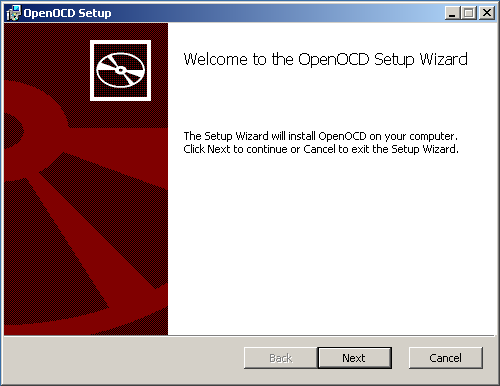
\includegraphics[width=0.7\textwidth]{../images/ch03/open-ocd-install-s1.png}}\hfill
 \subfloat{\label{fig:OpenOCD-B}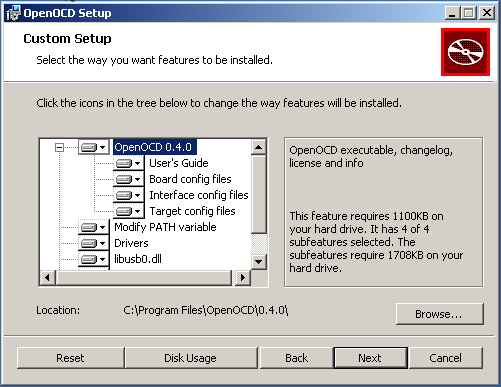
\includegraphics[width=0.7\textwidth]{../images/ch03/open-ocd-install-s2.png}}
 \caption{Instalator Open On-Chip Debugger'a (OpenOCD)}
 \label{fig:openocd-win32-install}
\end{figure}

Strona projektu OpenOCD dostępna jest pod adresem
\url{http://openocd.berlios.de/web/}. Dostępne są tam zarówno źródła jak i
dokumentacja do projektu. Niestety w chwili pisania pracy magisterskiej autorzy
nie udostępniali wersji skompilowanej dla systemu Windows. Dlatego też użyta
została niezależna wersja OpenOCD z przygotowanym instalatorem dla systemu
Windows. Instalator OpenOCD dla Windows jest do pobrania ze strony
\url{http://www.ethernut.de/en/download/}. Po uruchomieniu instalatora wybieramy
lokalizację docelową w której OpenOCD ma zostać zainstalowane. Po zakończeniu
instalacji konieczne jest uzupełnienie wartości zmiennej systemowej PATH ścieżką
do miejsca instalacji OpenOCD, domyślnie \url{C:\ethernut\nut\tools\win32}.

\subsection{Konfiguracja zintegrowanego środowiska programistycznego}
Poprawne zainstalowanie pakietów WinARM oraz OpenOCD dostarcza wszystkich
niezbędnych narzędzi potrzebnych do rozwijania aplikacji dla platform
wbudowanych. Niemniej jednak korzystanie z nich wymaga bezpośredniej interakcji
z linią poleceń systemu Windows, co dla niektórych programistów może być
uciążliwe. Możliwe jest napisanie skryptów systemowych pozwalających na
uruchamianie sekwencji procedur wymaganych np. do zaprogramowania robota,
ale jest to rozwiązanie nieprzenośne i słabo konfigurowalne. Dlatego też zaleca
się instalację zintegrowanego środowiska programistycznego które oprócz edytora
kodu umożliwi automatyzację najczęściej wykonywanych zadań. Wybór rodzaju
środowiska programistycznego zależy niemal w całości od preferencji programisty
gdyż większość potrzebnych narzędzi można bez większych trudności zintegrować z
ulubionym edytorem. Na potrzeby tej pracy omówiona zostanie konfiguracja dla
środowiska Eclipse. Wybór podyktowany został faktem iż jest to obecnie jedna z
najpopularniejszych platform do rozwoju oprogramowania, a co więcej jej
konfiguracja przebiega identycznie dla systemu Windows jak i Linux. Z tego
względu szczegółowy opis procedury konfiguracji zamieszczony został w rozdziale
poświęconym narzędziom dla systemu Linux.

\subsection{Narzędzia dla systemu Linux}
Jednym z wymagań pracy dyplomowej było przygotowanie zestawu narzędzi dla systemu
Linux, dzięki którym będzie możliwy dalszy rozwój robota. Zbiór programów
potrzebnych do rozwoju projektu to: zintegrowane środowisko programistyczne
(IDE), kompilator oraz oprogramowanie pozwalające zaprogramować mikrokontroler.
Bierzący rozdział opisuje sposób instalacji i wykorzystania poszczególnych
narzędzi, a także daje światło na inne tego typu oprogramowanie, które było brane
pod uwagę podczas pracy nad projektem, jednak nie zostało użyte.

\subsubsection{Wybór zintegrowanego środowiska programistycznego}
We wcześniejszej wersji oprogramowanie robota było rozwijane na systemie
Microsoft Windows. Niestety zintegrowane środowisko programistyczne używane do
tej pory nie jest multiplatformowe. Konieczne było zatem dobranie nowego IDE,
które umożliwiało będzie rozwijanie stworzonego wcześniej kodu pod systemem
Linux. Oczywiście biorąc pod uwagę niski budżet projektu, wszelkie płatne
rozwiązania zostały prawie  od razu odrzucone. Rozważaniom zostały poddane
następujące środowiska: Eclipse, Netbeans, CodeWarrior, Kile, ARM Workbench IDE.

\textcolor{red}{TODO: DLACZEGO NIE WYBRALIŚMY INNYCH ??}

Ostatecznie zostało wybrane środowisko Eclipse, które jest dostępne na zasadach
licencji: Eclipse Public License, odpowiadającej wymaganiom projektu.
Najwiekszymi zaletami tego rozwiazania jest łatwość instalacji, konfiguracji oraz
użytkowania. W podjęciu ostatecznej decyzji równie istotne było to, iż
rozwiązania płatne takie jak np. CodeWarrior są bazowane na Eclips'ie. Plusem był
także fakt iż dostępne są różnego rodzaju dodatki do Eclipse'a dedykowane do
rozwoju oprogramowania na mikrokontrolery ARM. Istalacja i sposób wykorzystania
jednego z nich został opisany w \textcolor{red}{ TODO: NUMER DODATKU!!!! },
chociaż nie był on wykorzystywany przez autorów tej pracy.

\subsubsection{Instalacja i konfiguracja Eclipse'a}
Wybrane środowisko programistyczne (Eclipse) jest udostępniane pod adresem:
\url{http://www.eclipse.org/downloads/}. Ściągnięte archiwum rozpakowujemy w
wybranym przez nas miejscu. Przechodzimy następnie do katalogu który został
wydobyty z archiwum i uruchamiamy Eclipse'a.

Oprogramowanie zaraz po pierwszym uruchomieniu zapyta nas o miejsce w którym będą
przechowywane źródła naszego projektu tzw. Workspace. Dobrym pomysłem jest
potwierdzenie ustawień domyślnych i zapamiętanie tej ścieżki.

\begin{figure}
 \centering
 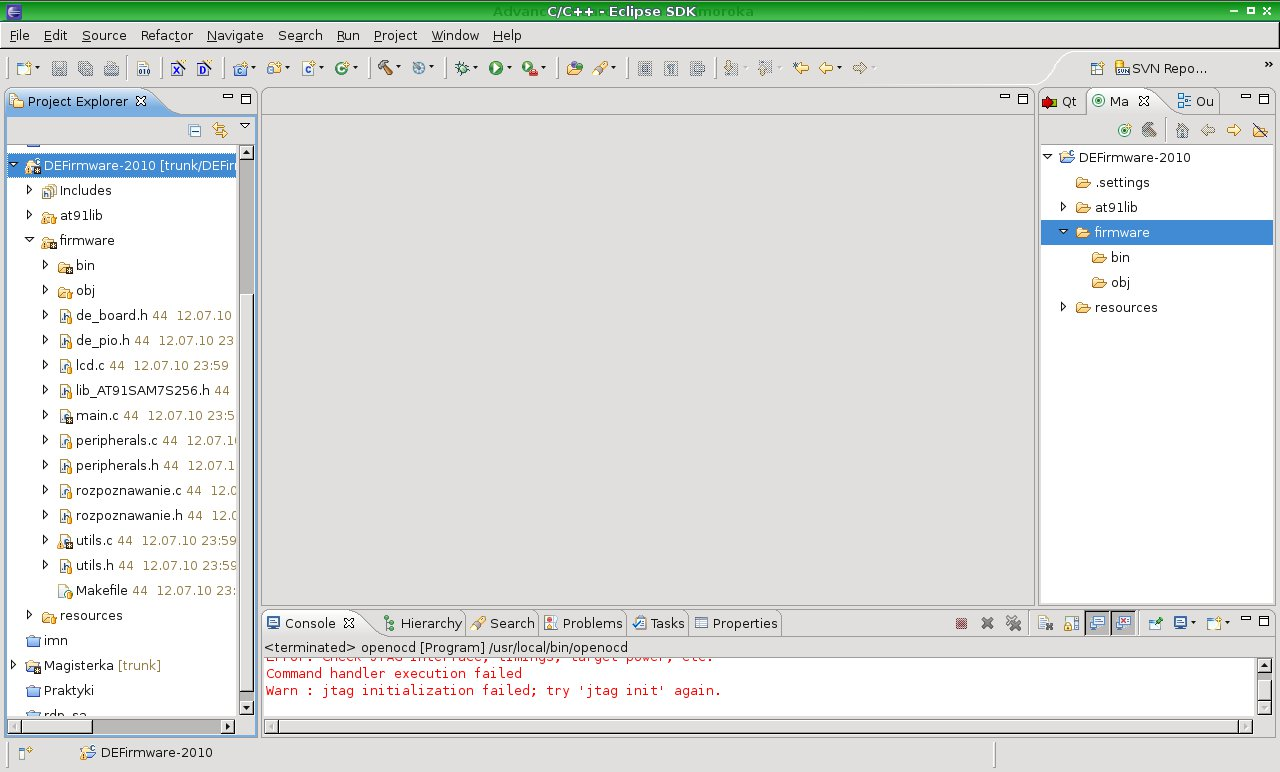
\includegraphics[width=150.0mm]{../images/Eclipse-MainWindow.jpg}
 \caption{Okno główne IDE Eclipse z dodanym projektem}
 \label{fig:Eclipse-MainWindow}
\end{figure}

\paragraph{Dodawanie projektu z firmware'm Dark Explorer'a}
Do workspace'u Eclipse'a należy skopować katalog z kodem sterującym robota.
Następnie dodajemy nowy projekt w IDE wybierając kolejno \textit{File --> New -->
C++ Project}. W oknie dialogowym \textit{C++ Project} (rysunek
\ref{fig:Eclipse-CPP-Project}), należy podać nazwę projektu która powinna być
zgodna z nazwą katalogu zawierającego kod robota. Następnie z listy Project type,
wybieramy \textit{Makefile project --> Empty Project}, a jako \textit{Toolchain}
wybieramy \textit{Other toolchain}. Całą operację zatwierdzamy przyciskiem
\textit{Finish}.

\begin{figure}
 \centering
 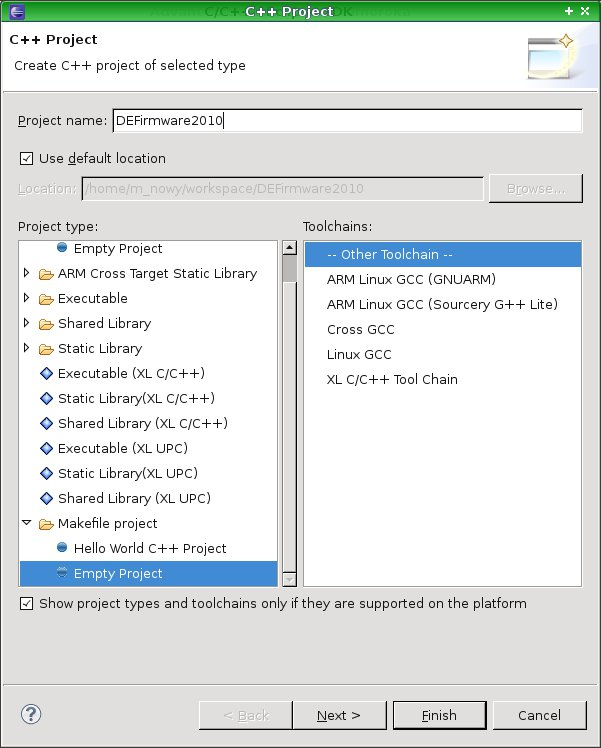
\includegraphics[height=100.0mm]{../images/Eclipse-CPP-Project.jpg}
 \caption{Okno dialogowe C++ Project}
 \label{fig:Eclipse-CPP-Project}
\end{figure}

Po poprawnym dodaniu projektu naszym oczom powinno się ukazać okno podobne do
tego na rysunku \ref{fig:Eclipse-MainWindow}

W przypadku gdy przed uruchomieniem Eclipse'a nie ustawilismy ścieżki do
odpowiedniego toolchain'a w zmiennych środowiskowych systemu. podjąć dodatkowe
kroki. Eclipse umożliwia konfigurowanie tych zmiennych dla pojedyńczych
projektów. W celu ustawienia wymaganej ścieżki klikamy prawym klawiszem myszy na
nazwie naszego projektu w \textit{Project Explorer'ze} i wybieramy
\textit{Properties}.

\begin{figure}
 \centering
 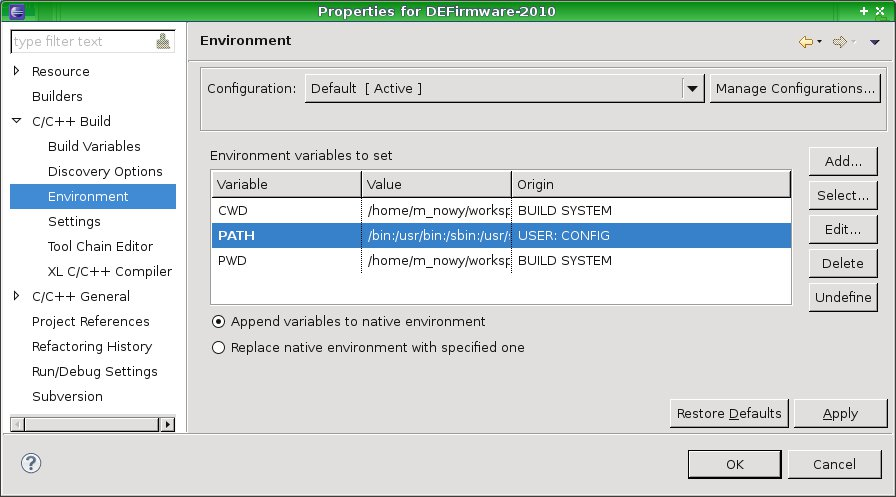
\includegraphics[width=150.0mm]{../images/Eclipse-Project-Properties.jpg}
 \caption{Okno dialogowe Properties}
 \label{fig:Eclipse-Project-Properties}
\end{figure}

Po ukazaniu się okna dialogowego \textit{Properties} (rysunek
\ref{fig:Eclipse-Project-Properties}) wybieramy \textit{C/C++ Build -->
Environment}. Następnie modyfikujemy zmienną \textit{PATH}, dodając na końcu
ścieżkę do naszego toolchain'a.

W celu przetestowania poprawności naszej konfiguracji możemy spróbować
skompilować kod, klikając prawym klawiszem myszy na nazwę projektu, a następnie
wybierając z menu kontekstowego opcję \textit{Build Project}. W wyniku powinniśmy
otrzymać dwa pliki binarne w katalogu \textit{firmware/bin}. Są to pliki gotowe
do umieszczenia w pamięci flash robota.

\subsubsection{Instalacja i konfiguracja toolchain'a}
W celu przetworzenia kodu do formy współpracującej z mikrokontrolerem ARM
niezbędny nam jest odpowiedni toolchain, czyli zestaw narzędzi generujących pliki
wykonywalne oraz pomagających w debugowaniu utworzonego oprogamowania. Tworzony
kod był kompilowany przy pomocy GNUARM toolchain w wersji 3.4.3 dostępnej na
stronie
\url{http://www.gnuarm.com/bu-2.15_gcc-3.4.3-c-c++-java_nl-1.12.0_gi-6.1.tar.bz2}

Po ściągnięciu archiwum ze strony producenta należy rozpakować je do dowolnego
katalogu, na potrzeby tej pracy załóżmy że będzie to katalog \url{/usr/local/} W
celu zapewnienia dostępu do toolchain'a wszystkim programom wskazane jest
dodanie ścieżki /usr/local/bin do zmiennej środowiskowej PATH (komenda 
\verb|export PATH=$PATH:/usr/local/bin|).

W celu sprawdzenia poprawności instalacji należy wykonać komende:
\begin{verbatim}
arm-elf-gcc --version 
\end{verbatim}
której wynikiem powinien być komunikat podobny do tego na rysunku \ref{fig:arm-elf-gcc-test}.

\begin{figure}
 \centering
 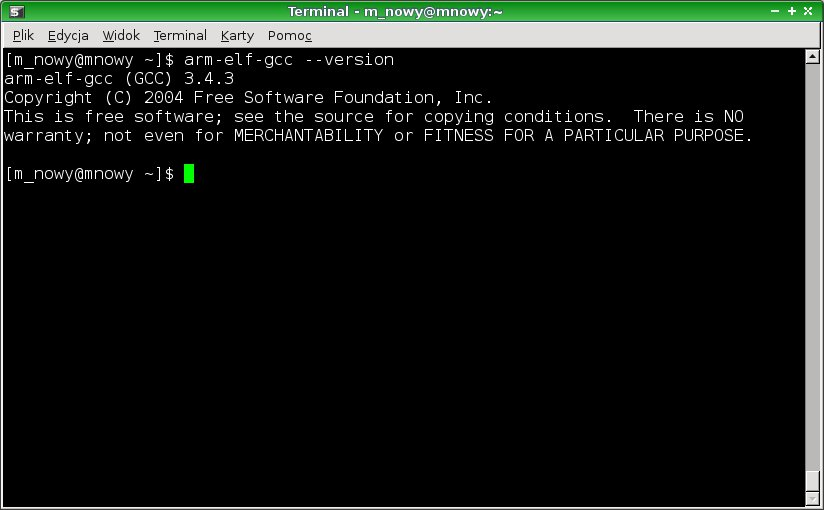
\includegraphics[width=150.0mm]{../images/arm-elf-gcc-test.jpg}
 \caption{Okno pokazujące odpowiedź prawidłowo zainstalowanego kompilatora}
 \label{fig:arm-elf-gcc-test}
\end{figure}

Trzeba wziąć pod uwage to, iż toolchain o którym mowa był przygotowany pod system
32--bit'owy. W przypadku konfiguracji na systemie 64--bit'owym konieczne jest
zaopatrzenie się w 64--bit'ową wersje binarną toolchain'a lub skompilowanie go
samodzielnie. Ewentualne dodatkowe informacje można znaleźć pod adresem
\url{http://www.gnuarm.com}.

\subsubsection{Open On--Chip Debugger -- instalacja i konfiguracja}
\label{roz:opendocd-install}
Pamięć robota była programowana przy pomocy tego samego narzędzia które służy do
sprawdzania poprawności działania napisanego kodu. Mowa tu o oprogramowaniu Open
On--Chip Debugger.

Źródła programu należy pobrać ze strony:
\url{http://sourceforge.net/projects/openocd/}. Autorzy programu nie zamieścili
wersji binarnych, wiec kompilacje będziemy musieli przeprowadzić sami.

Po ściągnieciu i rozpakowaniu źródeł uruchamiamy skrypt configure z odpowiednimi
argumentem'ami przy pomocy komendy:

\begin{verbatim}
./configure --prefix=/usr/local --enable-ft2232_libftdi 
\end{verbatim}

Dodatkowy argument powoduje włączenie obsługi urządzeń bazujących na układzie
FT2232 urzywając biblioteki libftdi. Jest to niezbędne przy korzystaniu z
programatora Triton JTAG A. W przypadku wykorzystywania programatora innej firmy
możliwa będzie konieczność wprowadzenia innego argumentu do skryptu
konfiguracyjnego. Argument prefix określa ścieżke docelową instalacji
oprogramowania.

Gdy skrypt konfiguracyjny zakończy działanie z powodzeniem, możemy wywołać
komende \verb|make && make install| w celu kompilacji i instalacji
oprogramowania.

Po zakończeniu powyższych czynności należy skopiować plik (\textcolor{red}{TODO:
triton.cfg Czy trzeba podawać dokładną ścieżke? płyta? www?}) konfigurujący
połączenie przy pomocy programatora Triton JTAG A do katalogu
\url{/usr/local/openocd/interface}.

W celu przetestowania działania Open On--Chip Debugger'a należy podłączyć
programator Triton JTAG A do portu usb komputera oraz portu JTAG robota. Po
upewnieniu się że robot jest włączony wykonujemy komende:

\begin{verbatim}
openocd -s /usr/local/share/openocd/scripts -f board/atmel_at91sam7s-ek.cfg
-f interface/triton.cfg 
\end{verbatim}

\begin{figure}
 \centering
 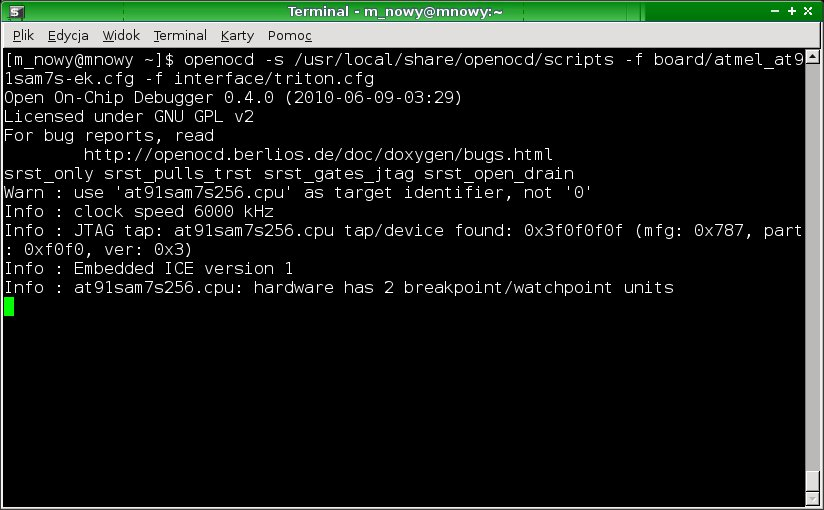
\includegraphics[width=150.0mm]{../images/openocd.jpg}
 \caption{Poprawnie uruchomiony openocd}
 \label{fig:openocd}
\end{figure}

\paragraph{Programowanie pamięci Dark Explorer'a}
W celu wgrania programu do pamięci robota musimy uruchomić dwa narzędzia: telnet
oraz openocd. Procedura instalacji i uruchamiania openocd została opisana
wczesniej w rozdziale \ref{roz:opendocd-install}. W pierwszym kroku uruchamiamy
openocd w celu podłączenia się do robota. Następnie startujemy telnet za pomocą
polecenia:

\begin{verbatim}
 telnet localhost 4444
\end{verbatim}

Zapewnia nam to możliwość wysyłania komend sterujących do openocd. W celu
zaprogramowania pamięci flash Dark Explorer'a i uruchomienia nowej wersji
firmware'u należy wykonać zestaw komend:

\begin{verbatim}
 halt
 flash write_image {ścieżka_do_pliku_elf}
 reset init
 resume
\end{verbatim}

Natomiast w przypadku programowania pamięci RAM robota wykonujemy następujący
zestaw poleceń:

\begin{verbatim}
 halt
 load_image {ścieżka_do_pliku_bin} {początkowy_adres_pamięci}
 reset init
 resume
\end{verbatim}

\newpage
\chapter{Środowisko rozwojowe dla komputerów stacjonarnych}
\begin{figure}[!ht]
 \centering
 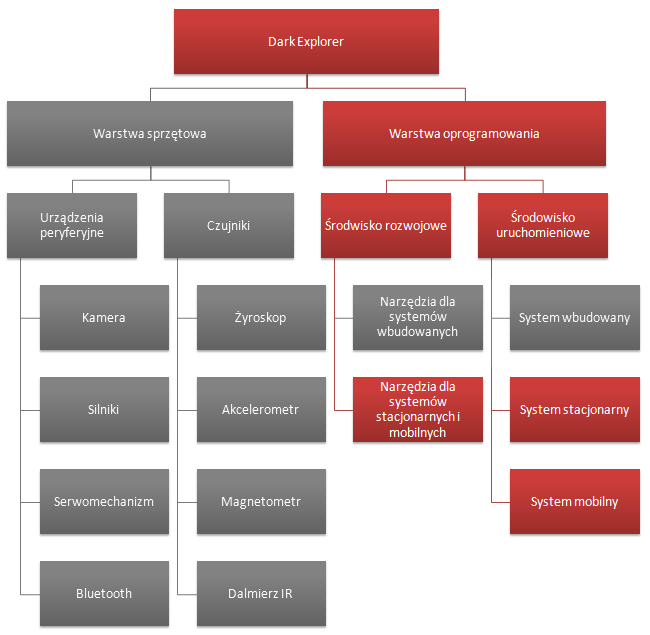
\includegraphics[height=125mm]{../images/ch03/dark_explorer_platform_ide_stac_mob.png}
 \caption{Struktura platformy robota mobilnego po zakończeniu prac. Kolorem oznaczono zakres prac opisanych w bierzącym rozdziale.}
 \label{fig:DarkExplorerPlatformStacMob}
\end{figure}

\section{Biblioteka zarządzająca dla języka Java}
\subsection{Bluetooth a Java SE}
\subsection{Opis możliwości biblioteki}
\section{Aplikacja zarządzająca na komputery stacjonarne (Java)}
\section{Biblioteka programistyczna dla platformy .NET}
Jednym z poważniejszych problemów zauważonych podczas analizy pierwotnej
konfiguracji robota był brak bibliotek umożliwiających tworzenie oprogramowania
które pozwalałoby na dowolne wykorzystanie możliwości oferowanych przez
konfigurację sprzętową robota. Brak tego rodzaju narzędzi znacząco ogranicza
możliwości rozwoju robota gdyż każda próba tworzenia nowego oprogramowania wymaga
od programisty zagłębiania się w szczegóły implementacji systemu wbudowanego
który kontroluje działanie robota. Aby usunąć tak poważne ograniczenie
zaprojektowana została biblioteka mająca na celu udostępnienie narzędzi
pozwalających programiście na skupienie się jedynie wysokopoziomowej
funkcjonalności bez konieczności szczegółowej analizy protokołu komunikacji i
zasad działania poszczególnych funkcji robota.

Przed przystąpieniem do implementacji konieczne jest podjęcie rozważnej decyzji z
wyborem środowiska i języka programowania w jakim biblioteka zostanie napisana.
Biorąc pod uwagę ciągle rosnącą popularność obiektowych języków programowania
oczywistym wydaje się być wybór języka właśnie z tej rodziny. Decydującym
aspektem, wpływającym na ostateczny wybór docelowej platformy rozwojowej, jest
więc ilość dostępnych bibliotek oraz przenośność kodu pomiędzy dostępnymi na
rynku platformami sprzętowymi. Po przeprowadzeniu wnikliwej analizy ostateczny
wybór padł na język C\# oraz platformę .NET. Wybór motywowany jest faktem iż
platforma .NET jest jednym z najdynamiczniej rozwijających środowisk
programistycznych ostatnich lat. Firma Microsoft dostarcza szereg bibliotek
dodatkowych oraz narzędzi pozwalających na szybkie tworzenie oprogramowania
działającego zarówno na urządzeniach mobilnych jaki i stacjonarnych. Dzięki
pracy programistów w ramach projektu Mono\footnote{Więcej informacji na temat projektu
Mono można znaleźć pod adresem strony internetowej http://www.mono-project.com/}
powstała platforma umożliwiająca uruchamianie aplikacji napisanych w języku C\#
nie tylko pod kontrolą systemu Windows, ale również pod systemami z rodziny Linux
i Mac. Dodatkowym atutem platformy .NET jest bardzo duża liczba bibliotek
dodatkowych dostarczanych przez środowiska programistów opensource.

W ramach pracy magisterskiej zaprojektowana została biblioteka programistyczna w
języku C\#. Docelową platformą uruchomieniową dla przygotowanej biblioteki są
systemy z rodziny Windows, Windows Mobile oraz Linux. Przy tworzeniu biblioteki
brane pod uwagę były najnowsze trendy w dziedzinie programistycznych wzorców
projektowych przy jednoczesnym zachowaniu spójności i uniwersalności kodu dla
poszczególnych środowisk uruchomieniowych. W wyniku implementacji powstała
wielowątkowa biblioteka oparta na zdarzeniach pozwalająca na dostęp do wszystkich
funkcji robota za pomocą intuicyjnego interfejsu programistycznego. Biblioteka
udostępnia szerokie spektrum metod pozwalających na swobodne sterowanie i
zarządzanie dostępnymi funkcjami robota. Wśród metod bibliotecznych znaleźć można
funkcje pozwalające na bezpośrednią interakcję z poszczególnymi podzespołami
bazowymi, jak również takie które umożliwiają wykonywanie predefiniowanych
sekwencji zadań przewidzianych przez autorów projektu. Biblioteka pokrywa swoją
funkcjonalnością nie tylko wsparcie dla wszystkich dostępnych roszerzeń
sprzętowych robota, ale również dostarcza interfejs pozwalający na automatyczną
obsługę połączenia z robotem z wykorzystaniem technologii bluetooth. Fakt ten
jest o tyle istotny, że proces komunikacji okazał się być najbardziej wrażliwym
elementem podczas migracji biblioteki pomiędzy poszczególnymi platformami
softwareowymi. Szczegółowa lista wszystkich dostępnych funkcji wraz z niezbędnym
komentarzem zamieszczona została w dodatku poświęconym kodu źródłowemu
stworzonego w ramach pracy magisterskiej. Taki sposób implementacji pozwala na
tworzenie oprogramowania współpracującego z nową wersją robota nawet przez osoby
nie posiadające dostatecznej wiedzy i umiejętności tworzenia oprogramowania do
obsługi systemów wbudowanych.

W ramach pracy magisterskiej stworzona została również przykładowa aplikacja
sterująca prezentująca wszystkie możliwości oferowane zarówno przez warstwę
aplikacyjną jak i sprzętową robota Dark Explorer. 

\textcolor{red}{TODO: zrzut ekranu aplikacji sterującej dla .net'a}

\newpage
\chapter{Środowisko rozwojowe dla urządzeń mobilnych}
\subsection{Platforma mobilna (Windows Mobile 6.1)}
Mobilne urządzenia przenośne z dnia na dzień zyskują na popularności. Każdego
dnia spotykamy się z nimi w domu, w pracy czy spacerując po parku. Z całą pewnością
można stwierdzić, iż większa część społeczeństwa obecnie jest w posiadaniu
telefonu komórkowego, komputera przenośnego czy też jakiegoś innego urządzenia
mobilnego. Wszystkie z wspomnianych urządzeń posiadają dedykowaną platformę
software'ową. Do najlepiej znanych we współczesnym świecie zaliczyć można między
innymi: Windows Mobile, iPhone, BlackBerry, Symbian OS, Android, Maemo, OpenMoko
itp. Każda z wymienionych platform posiada inną genezę jak również swoje mocne i
słabe strony.

Platformy takie jak Windows Mobile, BlackBerry czy iPhone ograniczone są do
urządzeń dedykowanych docelowo do współpracy z wspomnianymi środowiskami. Obok
różnorakich problemów z jakimi zmagają się wspomniane wcześniej platformy do
jednego z najpoważniejszych zaliczyć można bardzo ograniczone w niektórych
aspektach API. Nawet tak przenośna platforma jak Java na urządzeniach przenośnych
nie zawsze się sprawdza ze względu na liczne braki oraz różnice w API zmuszające
programistów do tworzenia kodu dedykowanego dla konkretnego urządzenia. Symbian
oraz Windows Mobile wypadają na tym tle nieco lepiej ponieważ wspierają szerszą
gamę urządzeń jak również ich API daje więcej możliwości niż ma to miejsce na
przykład w przypadku Javy. Głównym powodem takiego stanu rzeczy jest bardzo
szeroki i różnorodny asortyment platform sprzętowych utrudniający stworzenie
jednolitej i w pełni wykorzystującej wszystkie możliwości urządzenia platformy
programistycznej. Dostępne w chwili obecnej OpenSource'owe i wieloplatformowe
rozwiązania znajdują się ciągle we wczesnej fazie rozwoju i nie są jeszcze
powszechnie znane przez środowiska twórców oprogramowania.

Firma Microsoft wypuściła po raz pierwszy na światło dzienne swoją platformę
mobilną w latach 90-tych\cite{blog:wm-app-dev}. Natomiast w roku 2002 pojawiła
się pierwsza platforma Windows CE.NET. Zapoczątkowało to popularyzację urządzeń Pocket PC opartych o
system Windows CE 3.0 oraz późniejsze wersje. Dalszy rozwój bezprzewodowych
technologi telekomunikacyjnych pozwolił na integracje telefonu z komputerem
osobistym. Wspomniane urządzenia Pocket PC z 2002 roku wspierały między innymi
standard GSM, GPRS, bluetooth oraz umożliwiały użytkownikom dostęp do sieci
bezprzewodowych. W między czasie rozwojowi ulegały urządzenia typu SmartPhone
które koncepcyjnie były bardzo zbliżone do Pocket PC jednakże były one bardziej
zbliżone do telefonu niż komputera osobistego. Podstawową różnicą pomiędzy
Smartphone i Pocket PC jest fakt iż urządzenia Pocket PC posiadają ekran
dotykowy, a Smartphone wyposażone są jedynie w przyciski umożliwiające sterowanie
urządzeniem. Każde z tych urządzeń posiadało inny zestaw aplikacji pomocniczych
oraz wspierało inne standardy i technologie.
\newpage
W chwili obecnej większość urządzeń Pocket PC oraz Smartphone działają w oparciu
o system Windows Mobile 5 oraz Windows Mobile 6. Nowoczesne urządzenia Pocket PC
wyposażone są w procesor o taktowaniu 500-600 MHz oraz od 64-128 MB pamięci RAM.
Najnowsze urządzenia z tej grupy wyposażane są w 1 GHz procesor oraz 512 MB
pamięci.
 

\subsubsection{Środowisko rozwojowe}
Tworzenie aplikacji działających na urządzeniach pod kontrolą systemu Windows
Mobile jest niemal tak samo proste jak tworzenie zwykłych aplikacji na komputery
stacjonarne. Niemniej jednak do stworzenia w pełni funkcjonalnego środowiska
rozwojowego konieczne jest przejście przez klika kroków przygotowawczych
związanych z instalacją potrzebnych aplikacji narzędziowych. \\
\\
Przed rozpoczęciem przygody z tworzeniem aplikacji dla systemu Windows Mobile
konieczne jest zainstalowanie Microsoft Visual Studio. Zaleca się aby Visual
Studio było w wersji 2005 lub 2008. Niestety narzędzia umożliwiające rozwijanie
aplikacji mobilnych nie są poprawnie wykrywane przez Visual Studio 2010 oraz
poprzednie wydania w wersji Express. Dlatego też koniecznością jest instalacja
środowiska w wersji Standard lub Professional. Każda z tych wersji może zostać
pobrana w wersji czasowej ze stron firmy Microsoft lub w wersji pełnej z MSDNAA.
Visual Studio posłuży nam nie tylko do edycji kodu aplikacji ale pozwoli również
w prosty sposób budować, debugować oraz przygotować instalator finalnej wersji
aplikacji. Po poprawnym zainstalowaniu środowiska rozwojowego konieczne jest
pobranie i zainstalowanie dostępnych paczek serwisowych dostępnych dla wybranej
wersji Visual Studio. Pozwoli to uniknąć nieprzyjemnych niespodzianek podczas
instalacji bibliotek narzędziowych i późniejszej pracy.\\
\\
Jeżeli posiadamy już zainstalowaną kopię Visual Studio możemy przystąpić do
instalacji narzędzi pomocniczych które pomogą nam w tworzeniu aplikacji.
Pierwszą niezbędną biblioteką jest .NET Compact Framework 2.0 SP1. Jest to
zestaw narzędzi wykorzystywanych do uruchamiania aplikacji na platformach
opartych o Windows Mobile. Aby ułatwić sobie proces budowania, debugowania i
uruchamiania aplikacji na urządzeniu konieczne jest zainstalowanie w systemie
Windows ActiveSync. Dzięki ActiveSync możliwe stanie się uruchamianie
projektowanej aplikacji, bezpośrednio z IDE, nie tylko na prawdziwym urządzeniu
ale również emulatorze. \\
\\
Ostatnim, ale i zarazem najważniejszym krokiem jest instalacja Windows Mobile
SDK. Na stronach firmy Microsoft dostępne są dwie wersje SDK, Standard oraz
Professional. Wersja Standard zawiera w sobie tylko wsparcie dla urządzeń z
Windows Mobile Classic lub Standard natomiast wersja Professional obejmuje
wszystkie dostępne środowiska. Wybór SDK można sprowadzić do następującej
zasady. Jeżeli zamierzamy tworzyć oprogramowanie dla urządzeń Smartphone bez
ekranu dotykowego w zupełności wystarczy nam wersja standardowa. Jeżeli
natomiast planujemy napisane aplikacje uruchamiać na PocketPC lub dotykowych
SmartPhon'ach będziemy potrzebować bibliotek systemu Windows Mobile Classic lub
Professional, tak więc konieczne jest użycie SDK w wersji Professional. Tak jak
w przypadku Visual Studio, również tutaj zaleca się instalację wszystkich
dostępnych na stronie producenta aktualizacji i poprawek. Jest to szczególnie
istotne podczas pracy z emulatorami urządzeń. Po zrealizowaniu tych kroków
otrzymujemy w pełni funkcjonalne środowisko do rozwoju aplikacji mobilnych dla
urządzeń smartphone.

\paragraph{Modele aplikacji}
Istnieje klika modeli rozwoju aplikacji dla Windows Mobile, a wybór docelowego
modelu został pozostawiony programiście. Pierwszy z nich służy do tworzenia
aplikacji w kodzie natywnym. Aplikacje pisane zgodnie z tym modelem cechują się
wysoką wydajnością, bezpośrednim dostępem do sprzętu oraz małym zużyciem
zasobów. Do rozwoju tego rodzaju aplikacji korzysta się z reguły ze środowiska do
rozwijania aplikacji z użyciem Embeded Visual C++. Główną wadą tego modelu jest
niska przenośność pomiędzy różnymi platformami zwłaszcza jeżeli aplikacja
korzysta z urządzeń specyficznych dla danego modelu urządzenia. Docelowo więc za
pomocą tego modelu tworzy się biblioteki i narzędzia ułatwiających tworzenie
bardziej skomplikowanych aplikacji. Jeżeli więc interesuje nas tworzenie
wysokopoziomowych aplikacji z GUI, skierowanych bezpośrednio do użytkowników,
zaleca się tworzenie tego typu aplikacji za pomocą kodu zarządzalnego z użyciem
takich języków jak C\# czy Visual Basic. Rozwijanie aplikacji w oparciu o kod
zarządzalny pozwala na stworzenie programu który będzie mógł w pełni
wykorzystywać możliwości oferowane przez Microsoft .NET Compact Framework.
Umożliwia to programiście tworzenie rozproszonych systemów mobilnych pracujących
zarówno w modelu ze stałym połączeniem jak i bez. Spora część narzędzi
dostępnych w ramach .NET Compact Framework jest również wykorzystywana do rozwoju
aplikacji na komputery stacjonarne. Biblioteka została zaprojektowana docelowo na
urządzenia o ograniczonych zasobach co w połączeniu z możliwościami języków z
rodziny .NET oraz integracją z Visual Studio daje nam profesjonalny zestaw
narzędzi do tworzenia aplikacji mobilnych.
\\
Trzecim modelem tworzenia programów pod Windows Mobile jest wykorzystywanie kodu
serwera do pracy z wieloma różnymi typami urządzeń poprzez jeden wspólny kod
bazowy i model cienkiego klienta. Oczywiście tego typu podejście ma sens jedynie
gdy możemy zagwarantować stabilny kanał komunikacyjny pomiędzy urządzeniem
klienta, a serwerem. Każdy z przedstawionych modeli idealnie sprawdza się jeżeli
tylko w prawidłowy sposób wybierzemy model najbardziej odpowiadający potrzebom
naszej aplikacji.

\paragraph{Graficzny interfejs użytkownika}
Dzięki wygodnemu systemowi projektowania GUI
dostępnego w Visual Studio tworzenie interfejsu
użytkownika dla platformy mobilnej jest niemal tak proste jak w przypadku
tradycyjnych aplikacji, a jedyną różnicą jest ilość i rodzaj dostępnych
kontrolek. Różnice te wynikają z faktu iż niektóre urządzenia mobilne posiadają
ekrany dotykowe, a inne nie. Co za tym idzie, rozwój interfejsu użytkownika
staje się bardziej skomplikowany zwłaszcza jeżeli interesuje nas rozwój
aplikacji wspólnej dla obydwóch platform sprzętowych. W tym miejscu nie może
zabraknąć informacji, że oprogramowanie zbudowane dla PocketPC nie uruchomi się
na urządzeniach SmartPhone natomiast sytuacja odwrotna jest możliwa do momentu w
którym aplikacja nie zacznie korzystać ze specyficznych funkcji SmartPhone.
Naturalnym stanem rzeczy wydaje się fakt, iż wiele funkcji i komponentów
graficznych znanych z aplikacji desktopowych zostało usunięte z bibliotek
Windows Mobile, aby zapewnić jej wydajność i niewielki rozmiar. Dlatego też
pozostawiono tylko niezbędne, najprostsze komponenty. Ponieważ wydajność  i
zasoby pamięciowe urządzeń stale rosną, również ilość narzędzi dostępnych w SDK
jest systematycznie zwiększana, a co za tym idzie różnice pomiędzy kolejnymi
wersjami .NET Compact Framework są bardzo duże. Dlatego też posiadanie jak
najbardziej aktualnej wersji SDK ma niebagatelne znaczenie dla wygody tworzenia
aplikacji. Podsumowując rozwój GUI dla platformy mobilnej nie różni się bardzo
od tworzenia interfejsu użytkownika dla aplikacji dekstopowej. Istnieje również
możliwość rozwijania GUI w oparciu o silniki 3D. W chwili obecnych dostępne są
takie rozwiązania jak GAPI (Game API), OpenGL ES (Embeded Systems), Open VG
(Vector Grapics). Jednakże rozwój takich aplikacji jest niezwykle trudny gdyż
wymaga od programisty tworzenie maksymalnie optymalnego kodu, ze względu na
ograniczone możliwości niektórych urządzeń. 

\paragraph{Komunikacja}
Nowoczesne urządzenia mobilne posiadają szeroką gamę możliwości komunikacyjnych.
Posiadają one dostęp do szybkich sieci bezprzewodowych w standardzie 802.11
WiFi. Umożliwiają one również komunikację za pomocą portu podczerwieni,
bluetooth czy USB. Podejmując decyzję na temat wyboru kanału komunikacji należy
brać pod uwagę nie tylko parametry techniczne, ale również liczbę standardów i
protokołów dostępnych dla danego kanału komunikacji. Firma Microsoft dostarcza
szereg interfejsów programistycznych (API) umożliwiających niemal błyskawiczny
dostęp do funkcji komunikacyjnych urządzenia. AcitveSync API dostarcza funkcjonalność
umożliwiającą komunikację za pomocą protokołu synchronizacji. Natomiast
Bluetooth API dostarcza zestaw narzędzi umożliwiających nawiązywanie komunikacji
bezprzewodowej pomiędzy telefonami jak i urządzeniami peryferyjnymi.  API
Managera połączeń dostarcza zestaw usług umożliwiających automatyzację procesu
nawiązywania połączenia oraz zarządzanie ich aktywnością. API wymiany obiektów
(OBEX API) dostarcza funkcjonalność umożliwiającą wymianę danych pomiędzy
urządzeniami za pomocą efektywnego, kompaktowego protokołu binarnego
dedykowanego dla urządzeń z ograniczonymi zasobami. Remote API (RAPI) dostarcza
funkcję do zarządzania oraz zdalnego wywoływania metod po stronie
urządzenia klienta. Dostępne są m.in. funkcje dostępu do rejestru, plików, bazy
danych czy też konfiguracji urządzenia. Najważniejszą funkcjonalnością jest
jednak możliwość zdalnego wywoływania procedur. Za pomocą funkcji
CeRapiInvoke() przesyłamy do urządzenia nazwę biblioteki dynamicznej wraz z
nazwą metody która ma zostać wywołana na urządzeniu mobilnym. Kolejnym zestawem
narzędzi jest Pocket Outlook Object Model API dostarcza funkcje do zarządzania
obiektami Pocket Outlook  co umożliwia synchronizację zadań, kalendarza czy
kontaktów za pomocą prostego i intuicyjnego interfejsu. Dostępne jest również
Telephony API (TAPI) które zawiera w sobie biblioteki umożliwiające zarządzanie
kartą SIM oraz wiadomościami SMS. TAPI udostępnia również zestaw funkcji
umożliwiających dostęp do funkcji telefonowania oraz protokołu WAP. Nie
zabrakło również narzędzi do pracy z portami USB oraz COM. Część z dostępnych portów COM
jest zarezerwowana dla urządzeń wewnętrznych, ale pozostałe dostępne są do
pełnej dyspozycji użytkownika.

\paragraph{Debugowanie}
Microsoft Visual Studio umożliwia debugowanie aplikacji działających pod
kontrolą Windows Mobile w taki sam sposób jak ma to miejsce w przypadku
tradycyjnych aplikacji desktopowych. Ponadto programista ma do swojej
następujące narzędzia: emulator, panel zarządzania emulowanymi urządzeniami,
panel punktów przerwań i wątków. Niestety w Visual Studio nie uda się nam
jednocześnie debugować kodu natywnego i zarządzalnego. Możliwe jest natomiast
uruchomienie zarówno projektu napisanego w Visual C++ jak i projektu opartego o
kod zarządzalny, a dzięki funkcjonalności ,,Dołącz do procesu'' możliwe jest
zdalne dołączenie się doi monitorowanie procesu działającego na urządzeniu lub
emulatorze urządzenia. Narzędziem umożliwiającym komunikację pomiędzy
urządzeniem a systemem jest ActiveSync instalowany wraz ze środowiskiem
rozwojowym.  Za pomocą narzędzia ActiveSync możemy łączyć się nie tylko z
rzeczywistymi urządzeniami ale również z emulatorami. Umożliwia to pełną
wirtualizacje urządzeń mobilnych i znacznie ułatwia testowanie funkcjonalności
zwłaszcza pomiędzy różnymi platformami urządzeń (SmartPhone, PocketPC). Jedynym
ograniczeniem tego procesu jest możliwość utrzymania tylko jednego aktywnego
połączenia co uniemożliwia debugowanie na wielu urządzeniach jednocześnie. Co
więcej Visual Studio umożliwia debugowanie jedynie aplikacji stworzonej przez
programistę, nie możliwa jest z poziomu IDE debugowanie aplikacji i usług
systemowych działających na urządzeniu. Do tego typu debugowania konieczne
byłoby zbudowanie własnej wersji systemu Windows Mobile przy użyciu Platform
Buildera. Narzędzie to umożliwia również tworzenie własnego SDK dla Visual
Studio i platformy Windows CE. Dodatkową możliwością dostępną z poziomu
emulatora jest emulowanie połączenia z siecią GSM oraz wsparcie dla GPS.
Umożliwia to testowanie, debugowanie i rozwijanie szerokiego spektrum aplikacji
bez konieczności posiadania urządzenia fizycznie.

\subsubsection{Środowisko uruchomieniowe}
\section{Platforma mobilna (Java ME)}
Jednym z elementów rozwoju możliwości robota mobilnego Dark Explorer było stworzenie aplikacji zarządzającej na urządzenia przenosne. W ramach tego zadania stworzono aplikację działającą na platformie Java ME\footnote{Java ME - Java Micro Edition}. Platforma ta jest dedykowana dla aplikacji tworzonych na urządzenia mobilne o bardzo ograniczonych zasobach, takich jak telefony komórkowe. 

W związku z niską wydajnością procesorów oraz małą ilością pamięci w telefonach komórkowych Java ME posiada ograniczony w stosunku do Java SE\footnote{Java SE - Java Standard Edition, wersja platformy Java na komputery stacjonarne} zbiór klas nazywanych konfiguracją. W Java ME wyróżniamy twa typy konfiguracji: CDC\footnote{CDC -- Connected Device Configuration} dla urządzeń o lepszych parametrach (smartphone'y) oraz CLDC\footnote{CLDC -- Connected Limited Device Configuration} dla urządzeń o słabych parametrach (proste telefony komórkowe). W tej pracy wykorzystana została konfiguracja CLDC.

Konfiguracje Java ME są uzupełniane przez profile MIDP\footnote{MIDP -- Mobile Information Device Profile} które dodają swoje własne klasy do klas istniejących w konfiguracji. Klasy te zapewniają wykonywanie odpowiednich zadań na konkretnych elementach urządzenia mobilnego. Aplikacje wykorzystujące MIDP nazywane są MIDletami i są uruchamiane w środowisku KVM\footnote{KVM - K Virtual Machine}.

K Virtual Machine jest niczym innym jak wirtualną maszyną Java opracowaną dla konfiguracji CLDC. Jest ona bardzo ograniczona przez co posiada mniejsze wymagania sprzętowe w porównaniu ze swoimi odpowiednikami z komputerów klasy PC. Każdy producent urządzeń mobilnych musi zadbać o własną implementację maszyny wirtualnej na której będą uruchamiane MIDlety.
\subsection{Narzędzia programistyczne}

\subsection{Aplikacja mobilna}

\newpage
\chapter{Rozwój warstwy sprzętowej}
\section{Inercjalny system nawigacyjny}
W celu rozwinięcia możliwości robota, zamontowano w nim elementy przy pomocy
których, została podjęta próba stworzenia inercjalnego systemu nawigacyjnego
(INS\footnote{Inertial Navigation System}). Założeniem było, aby robot mobilny
był w stanie zapamiętać tor ruchu po jakim się porusza, gdy jest niesiony na ręce
osoby operującej nim. Następnie na podstawie wykonanych pomiarów robot miał
powrócić po zapamiętanym torze w miejsce początkowe. Elementy użyte do wykonania
INS zostały wybrane pod kątem walorów ekonomicznych. Nie były przeprowadzane
testy porównawcze pomiędzy podzespołami danego typu. Poniższy rozdział omawia
pokrótce czym jest INS, opisuje zasadę działania jego elementów oraz sposób
wykorzystania tych podzespołów do osiągnięcia wystarczająco dobrych efektów.

\subsection{Wprowadzenie do INS}
% http://citeseerx.ist.psu.edu/viewdoc/download?doi=10.1.1.63.7402&rep=rep1&type=pdf

Inercjalny system nawigacyjny jest to narzędzie służące do określenia położenia,
prędkości oraz orientacji obiektu w przestrzeni, bez korzystania z żadnych
zewnętrznych elementów naprowadzających, które byłyby dla niego punktem
odniesienia. Wykorzystuje on jedynie elementy wbudowane, składające się na
inercjalną jednostkę pomiarową (IMU\footnote{Inertial Measurement Unit}).
Inercjalne systemy nawigacyjne mają zastosowanie tam, gdzie jest potrzebna
informacja o aktualnym położeniu obiektów, natomiast nie ma możliwości odbioru
sygnału zewnętrznego, wymaganego do działania na przykład urządzeń GPS. Systemy
tego typu są stosowane w: samolotach, statkach, łodziach podwodnych, pojazdach
bezzałogowych czy statkach kosmicznych. Rozwój miniaturowych układów
elektromechanicznych MEMS\footnote{MEMS ?? } otworzył przed nami cały
wachlarz potencjalnych nowych zastosowań INS, np. do śledzenia ruchów ludzi bądź
zwierząt.

System nawigacyjny o którym mowa w tym rozdziale oblicza swoje położenie na
podstawie ciągłego badania przyspieszenia liniowego oraz prędkości kątowej. INS
musi otrzymać na starcie wartości początkowe położenia oraz prędkości z jaką się
porusza, aby móc zacząć wyznaczać dalsze przemieszczenie i zmiany w orientacji.

Robot mobilny został wyposażony w IMU składające się z następujących elementów
MEMS: żyroskopu oraz akcelerometru trójosiowego, a także magnetometru
dwuosiowego. Zasada działania poszczególnych elementów oraz opis ich
wykorzystania można znaleźć w kolejnych podrozdziałach.

\section{Akcelerometr trzyosiowy}
W latach 90 akcelerometry instalowano jedynie w roli mechanizmów służących do
uruchamiania poduszek powietrznych w samochodzie w przypadku wystąpienia
zderzenia. W chwili obecnej akcelerometry wykonane w technologii
MEMS można znaleźć w większości urządzeń codziennego użytku tj.
telefony komórkowe, konsole do gier, komputery przenośne czy cyfrowe aparaty
fotograficzne. Powodem tak spektakularnego wzrostu popularności było pełne
rozwinięcie się technologii MEMS. W dobie miniaturyzacji fakt, iż w miejsce do
niedawna używanych urządzeń można wstawić pojedynczy układ
scalony jest jednym z podstawowych powodów dla których, między innymi,
akcelerometry cieszą się tak szerokim spektrum zastosowań. Jednakże, ceną tak
daleko idącej miniaturyzacji jest spadek duży dokładności pomiarowej w
porównaniu do akcelerometrów opartych o tensometry. Jak się jednak okazuje, do
codziennego użytku precyzja oferowana przez tego typu czujniki jest w zupełności wystarczająca.

Bardzo dobrym przykładem zastosowania akcelerometru jest dostępna w większości
aparatów cyfrowych funkcja optycznej stabilizacji obrazu (Optical Image
Stabilization). Funkcja ta polega na redukcji zniekształceń  spowodowanych
drżeniem rąk fotografa w~trakcie akwizycji obrazu. Problem jest tym poważniejszy
iż nieustanna miniaturyzacja urządzeń dodatkowo wzmacnia mimowolne\footnote{Ręka
przeciętnego człowieka drży mimowolnie z częstotliwością od 10 do 20 Hz} drżenie
rąk użytkownika. Dlatego też większość aparatów wyposażonych jest czujniki które
mierzą wspomniane drgania, a następnie uzyskane informacje przekazują do modułu
sterującego położeniem soczewek i przetwornika obrazu. Następnie moduł ten
dostosowuje parametry pracy aparatu tak aby zminimalizować wpływ nieporządanych przeunięć
na efekt końcowy pracy jakim jest zdjęcie.

Innym popularnym przykładem zastosowania akcelerometrów są pedometry, potocznie 
nazywane krokomierzami. Dzięki zastosowanej technologii czujniki w krokomierzach
mogą dokonywać równocześnie pomiaru względem trzech osi. Co więcej tego typu
urządzenia umożliwiają dokonywanie pomiarów niemal całkowicie niezależne od
swojej orientacji, a ich niewielkie rozmiary pozwalają na ich integrację z 
dowolnymi urządzeniami mobilnymi. Akcelerometry wykonane w technologi MEMS
najlepiej sprawdzają się  podczas pomiaru przyspieszenia statycznego
pozwalającego jednoznacznie wyznaczyć kąt odchylenia urządzenia względem pionu. 
Można nimi dokonywać również pomiaru przyspieszenia dynamicznego pojawiającego 
się na skutek wibracji, uderzenia czy innego rodzaju ruchu. 

Niestety, pomimo swoich licznych zalet akcelerometry MEMS posiadają pewne
ograniczenia które mogą być bardzo istotne podczas projektowania bardziej
skomplikowanych systemów. Jedynym z podstawowych problemów jest brak możliwości
uzyskania jednoznacznej informacji na temat orientacji urządzenia zarówno w
pionie jak i poziomie. W~ramach przykładu spróbujmy przeanalizować wykorzystanie
akcelerometru do przełączania widoku na ekranie w zależności od jego orientacji. 
W~przypadku gdy oś X lub Y są równoległe z wektorem grawitacji na podstawie
informacji z akcelerometru można w~bardzo prosty sposób ustalić w~jakim
położeniu znajduje się aktualnie urządzenie.

\begin{figure}[h!]
 \centering
 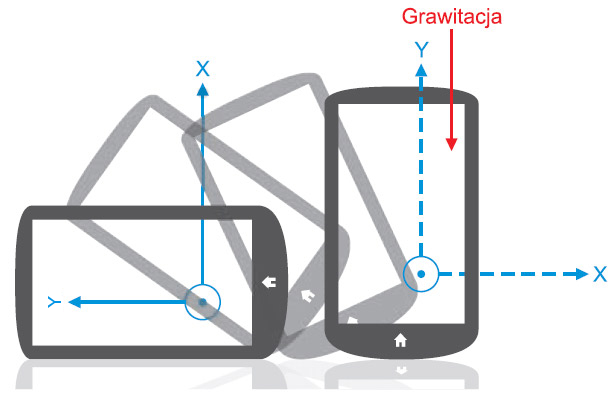
\includegraphics[height=75mm]{../images/ch04/acc_orientation.png}
 \caption{Pokrywanie się osi ekranu z kierunkiem wektora grawitacji pozwala na
 precyzyjne wyznaczenia orientacji urządzenia\cite{website:elektronikab2b-zyroskop}}
 \label{fig:AkcelerometrOrientation}
\end{figure}

Natomiast w przypadku gdy osie ekranu ustawią się prostopadle do wektora
grawitacji dane pozyskane z akcelerometru nie pozwalają na wyznaczenie
jednoznacznej pozycji w jakiej znalazło się urządzenie\cite{website:elektronikab2b-zyroskop}. Co więcej w
przypadku aplikacji w których akcelerometr jest źródłem informacji o odchyleniu od pionu
konieczne jest rozdzielenie zmian związanych wpływem grawitacji od szumów
związanych z przyspieszeniem dynamicznym. Tak pozyskane informacje będą
służyć jako punkt odniesienia pozwalającego na wyznaczenie kąta wychylenia.
Głównym problemem jest fakt, że sygnał taki można wyróżnić jedynie w chwili gdy
akcelerometr jest w stanie spoczynku, co w przypadku niektórych rodzajów
zastosowań może dawać nieoczekiwane rezultaty i zachwiać stabilność pracy całego
systemu. 

Jeżeli założymy, że zmiany odpowiadające przyspieszeniu dynamicznemu mają dużą
częstotliwość to możemy przy użyciu filtru dolnoprzepustowego usunąć zakłócenia
związane z drganiami wywołanymi przez użytkownika. Oczywistą implikacją
powyższego założenia jest założenie, że zmiana kąta nachylenia względem pionu są
wolne. W przeciwnym wypadku informacja o zmianie odchylenia zostaną usunięte
przez wspomniany filtr. Aby pominięcie wspomnianych ograniczeń stało się możliwe
konieczne jest zastosowanie dodatkowych czujników takich jak np. żyroskop które
dostarczą uzupełniających informacji pozwalających na stabilną implementację
funkcjonalności.

\subsection{Rodzaje akcelerometrów}
Istnieje wiele różnych rodzajów akcelerometrów. Akcelerometry mechaniczne
przypominają po części zachowanie pasażera w samochodzie który gwałtowanie
przyspiesza i zwalnia. Posiadają one element masy przyczepiony do elementu
sprężynowego umieszczonego w całości w zewnętrznej obudowie. Kiedy taki
akcelerometr zacznie przyspieszać obudowa zewnętrzna przemieści się podczas gdy
punkt masy wychyli się w kierunku przeciwnym do przyspieszenia co spowoduje
rozciągnięcie się sprężyny wprost proporcjonalne do siły która spowodowała
przyspieszenie. Mierząc więc odległość na jaką nastąpiło wychylenie jesteśmy w
stanie wyznaczyć wartość działającej siły, a co za tym idzie również wartość
przyspieszenia. Opisana powyżej zasada pomiaru leży u podstaw działania
sesjsmografów które za pomocą masy dołączonej do elementu piśmiennego rejestrują
siły występujące w chwili trzęsienia ziemi.

Alternatywnym podejściem jest wykorzystanie sygnałów elektrycznych i
magnetycznych do pomiaru przyspieszenia. Wśród tego rodzaju akcelerometrów
możemy wyróżnić następujące trzy typy: akcelerometr piezorezystywny,
akcelerometr pojemnościowy oraz akcelerometr piezoelektryczny. Istnieją również
akcelerometry które dokonują pomiaru przyspieszenia w oparciu o efekt Halla. 

\begin{figure}[h!]
 \centering
 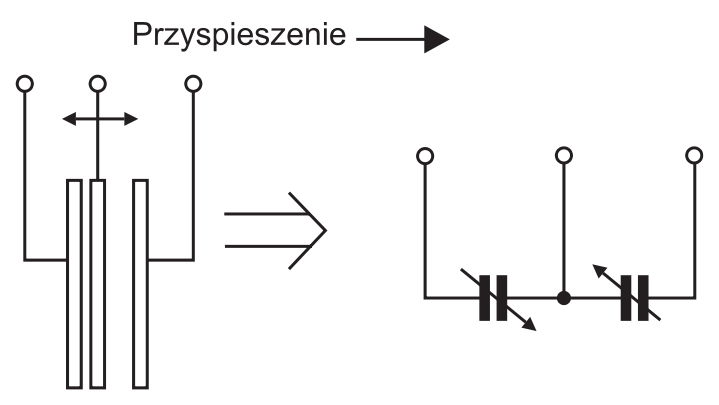
\includegraphics[height=62mm]{../images/ch04/acc_intro.png}
 \caption{Schemat ideowy akcelerometu pojemnościowego dokonującego pomiaru
 wzdłuż jednej osi\cite{ElektronikaPraktyczna22010}}
 \label{fig:AkcelerometrIdeowyScheamt}
\end{figure}

Przyspieszomierze piezorezystywne mają punkt masy dołączony do potencjometru
który zwiększa i zmniejsza przepływ prądu w zależności od siły jaka oddziałuje
na czujnik. Bardzo podobną zasadę działania wykazują akcelerometry pojemnościowe
te jednak wykorzystują efekt zmiany pojemności kondensatorów zastosowanych w
miejscu w którym poprzednio użyty został potencjometr. Ostatnim rodzajem
akcelerometrów są urządzeniami bazujące na piezoelektrycznych kryształach takich
jak na przykład kwarc. W urządzeniach tych punkt masy, pod wpływem
przyspieszenia, naciska na kryształ co powoduje, powstawanie napięcia które
jest wykorzystywane do wykonywania pomiaru. Cechą charakterystyczną tego rodzaju
czujników jest brak wskazań wartości przyspieszenia statycznego.\cite{website:elektronikab2b-platforma-bezzalogowa}

\subsection{Algorytm rozpoznawania kroków}
Do poprawnego działania algorytmu zaprezentowanego w ramach noty
aplikacyjnej\cite{Pedometer-haam326b} wymagane jest wykorzystanie akcelerometru
trójosiowego. Jak już wspomniano wcześniej, dzięki zastosowaniu urządzenia tego
typu jesteśmy w stanie wyeliminować problemy wynikające z konieczności 
uwzględnienia aktualnego wychylenia akcelerometru względem wektora grawitacji. 
W przypadku gdyby możliwe byłoby korzystanie tylko z pojedynczych osi poprawne
działanie algorytmu byłoby zapewnione jedynie w ściśle określonej pozycji co
jest znaczącym utrudnieniem biorąc pod uwagę niehomogeniczny charakter ruchów
wykonywanych podczas chodzenia. Aby wyeliminować wspomniany problem do
ostatecznego rozwiązania brana jest jedynie wartość stanowiąca złożenie wartości
przyspieszenia dla poszczególnych osi. Do wyznaczenia bezwzględnego
przyspieszenia na podstawie danych z osi X, Y, Z użyte zostało równanie
\ref{eq:AccCompositEq}.
\begin{equation}
a_{xyz} = \sqrt{{a_x}^2 + {a_y}^2 + {a_z}^2}
\label{eq:AccCompositEq}
\end{equation}
Zaimplementowany w ramach pracy magisterskiej algorytm wykrywania i zliczania
kroków bazuje na założeniu iż sumaryczna wartość przyspieszenia wykrywanego
przez akcelerometr w trakcie chodzenia oscyluje wokół wartości 1G\footnote{1G
- Jednokrotność przyspieszenia ziemskiego wynoszącego w przybliżeniu 9.81
$\frac{m}{s^2}$}. Podstawową zasadą działania algorytmu jest więc wykrywanie
cykli w jakich następuje kolejno spadek wartości odczytywanego przyspieszenia, a
następnie jego wzrost ponad wartość spoczynkową. Do poprawnego działania
algorytmu konieczne jest dobranie nie tylko odpowidniej stałej czasowej w której
wykryty cykl będzie zliczany jako krok, ale również ustalenie progów
przyspieszenia poniżej i powyżej wartości spoczynkowej które będą traktowane
jako odpowiednio początek i koniec cyklu.

\subsection{Implementacja algorytmu}
Do praktycznej implementacji algorytmu wykrywania kroków wykorzystany został
moduł akcelerometru trójosiowego firmy Freescale Semiconductor. Czujnik 
MMA7260\cite{MMA7260DataSheet} został zainstalowany w robocie jako element
modułu MOBOT-GM3A. Moduł akcelerometru jest to jedyny moduł w całości
dostarczony przez zewnętrznego dostawce, a wybór takiej strategii podyktowany
był jedynie względami ekonomicznymi i dostępnością tego typu urządzeń na polskim
rynku elektronicznym. Na ilustracji zamiszczone zostało zdjęcie gotowego układu
wraz z zaznaczonymi wyprowadzeniami.

\begin{figure}[h!]
 \centering
 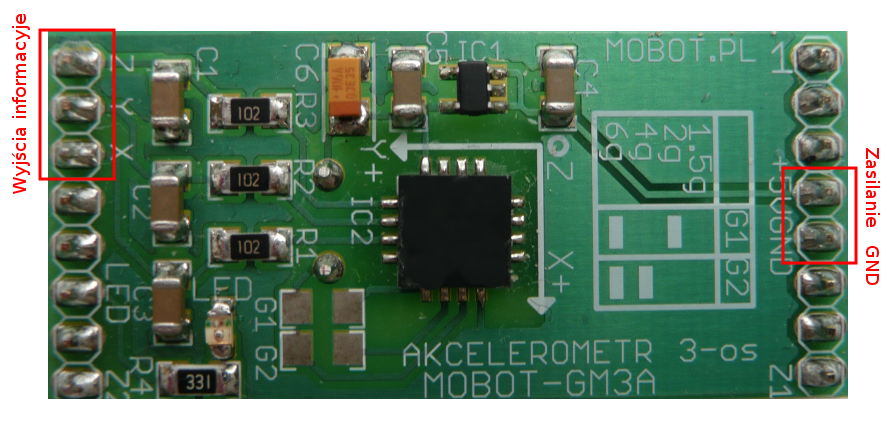
\includegraphics[height=76mm]{../images/ch04/gm3a_view.png}
 \caption{Moduł akcelerometru trójosiowego z czujnikiem przyspieszenia MMA7260}
 \label{fig:AccView}
\end{figure}

Wykorzystany czójnik przyspieszenia oferuje cztery zakresy czułości których
zmiana odbywa się poprzez konifguraję odpowiednich zworek w module MOBOT - GM3A.
W~ramach implementacji wybrany został zakres czułości od $-1.5g$ do $1.5g$ gdyż
udziela on najdokładniejszej informacji na temat przyspieszenia w przedziale w
jakim mieszczą się przyspieszenia związane z chodzeniem. W wybranym trybie
czułości akcelerometr wykazuje czułość rzędu 800mV/g, co przy wartości
przyspieszenia równej zero daje środek przedziału czułości na poziomie 1.65V.
Ze względu na analogową charakterystykę sygnału wyjściowego z modułu
akcelerometru konieczne jest wykorzystanie konwertera analogowo-cyfrowego w
celu odczytania danych pomiarowych otrzymywanych na wyjściach urządzenia.
Szczegółowy opis działania wbudowanego w robota ADC można znaleźć w rozdziale
poświęconym dalmierzom IR. 

\begin{figure}[h!]
 \centering
 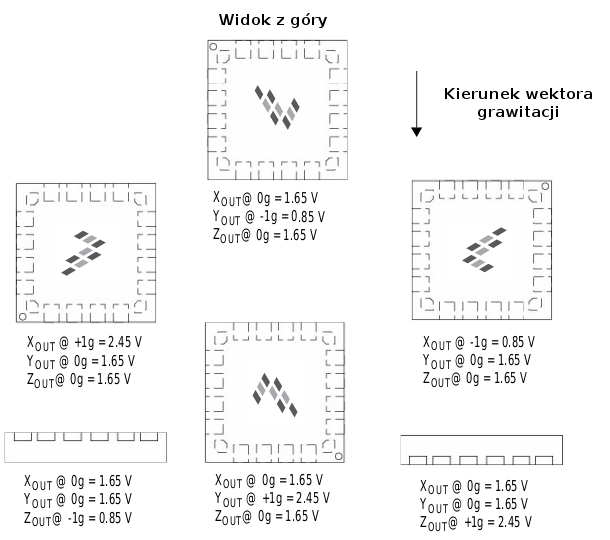
\includegraphics[height=75mm]{../images/ch04/mma7260_datasheet.png}
 \caption{Wartości przyspiesznia statycznego dla układu MMA7260 dostarczone w
 ramach specyfikacji technicznej urządzenia\cite{MMA7260DataSheet}}
 \label{fig:MMADataSheetStaticAcc}
\end{figure}

Przed rozpoczęciem praktycznej implementacji alogrytmu wykrywania kroków
konieczne okazało się przeprowadzenie kalibracji modułu, gdyż już wstępne testy
czujnika zwróciły spore różnice pomiędzy wartościami podanymi w nocie
katalogowej, a stanem zmierzonym na wyjściach akcelerometru. Zgodnie z rysunkiem
znalezionym w dokumentacji udostępnionej przez producenta czułość oraz zakres
napięć na poszczególnych osiach powinien być w stałych, jednakowych
przedziałach. Niestety jak się okazało poszczególne osie miały bardzo znaczące
różnice w zakresie swojej czułości co mogłoby bardzo niekorzystnie wpłynąć na
stabilność działania zaproponowanego algorytmu zliczania kroków. 

\begin{figure}[h!]
 \centering
 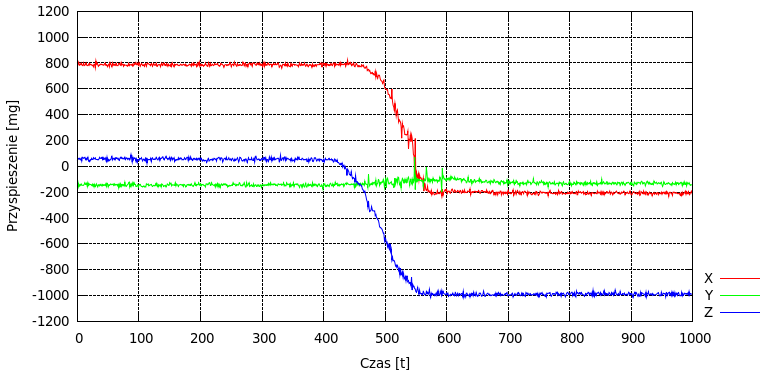
\includegraphics[height=80mm]{../images/ch04/raw_acc_data.png}
 \caption{Wartości przyspiezenia odczytywane na wyjściach akcelerometru przed
 przeprowadzeniem kalibracji}
 \label{fig:MMADataRaw}
\end{figure}

Wspomniany proces kalibracji polegał na ustawieniu czujnika na płaskiej,
poziomej powierzchni oraz odczytaniu wartości przyspieszenia statycznego dla
każdej z osi z osobna. Procedurę taką powtarzano wielokrotnie zmieniając
orientację modułu względem wektora grawitacji. Po zebraniu wszystkich danych
pomiarowych dla każdej osi z osobna została wyznaczona rzeczywista czułość, a
następnie w module odpowiedzialnym za akwicyzję danych o przyspieszeniu zostały
zaprogramowane funkcje korygujące otrzymane dane wejściowe o wartości wyliczone
podczas kalibracji urządzenia. Na poniższych wykresach znajdują się informacje o
stanie wyjść przed i po przeprowadzeniu kalibracji. 
  
\begin{figure}[h!]
 \centering
 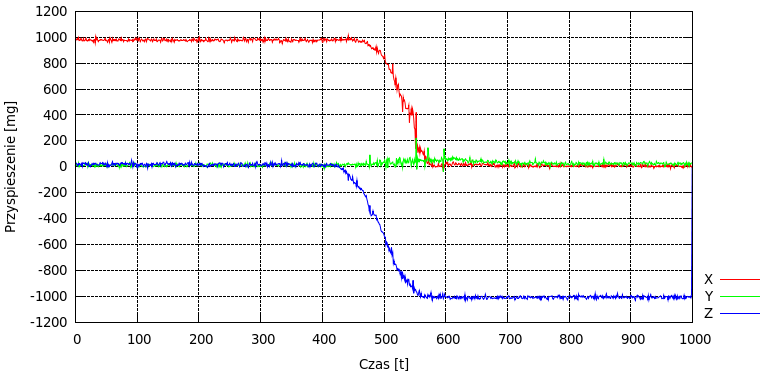
\includegraphics[height=80mm]{../images/ch04/calib_acc_data.png}
 \caption{Wartości odczytywane na wyjściach akcelerometru po przeprowadzeniu kalibracji}
 \label{fig:MMADataCalib}
\end{figure}
\subsection{Żyroskop}
Do budowy inercjalnej jednostki pomiarowej został użyty żyroskop trójosiowy L3G4200D firmy STMicroelectronics wykonany w
technologii MEMS. Element tego typu może być również wykorzystany podczas stabilizacji obrazu w aparatach cyfrowych lub
kontrolerach do gier.
\section{Magnetometr}
Jednym z elementów większości Inercjalnych Systemów Nawigacyjnych jest
magnetometr. Wykorzystuje się go do określenia kierunku w którym porusza się dane
ciało. Typów czujników mierzących pole magnetyczne jest wiele. Dla INS istotny jest jedynie czujnik, będący w stanie wykonać pomiary w zakresie indukcji pola magnetycznego ziemi, która wynosi od $30\mu T$ do $60\mu T$.
\\

\begin{figure}[!ht]
 \centering
 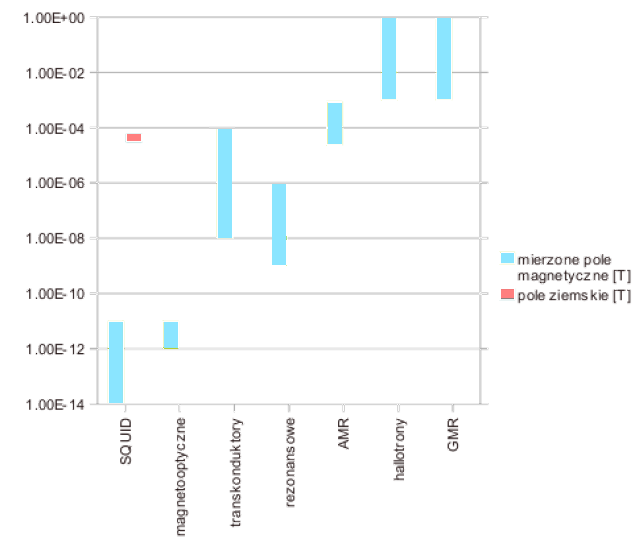
\includegraphics[height=100mm]{../images/ch04/magnetic_sens_types.png}
 \caption{Zakresy czujników pola magnetycznego różnego typu \cite{WstepnyProjektModuluIMU}}
 \label{fig:WykresMagnet}
\end{figure}

Na rysunku \ref{fig:WykresMagnet} przedstawione są zakresy pomiarowe czujników
pola magnetycznego różnego typu. Jak widać tylko dwa rodzaje magnetometrów z
wyżej wymienionych działają w przedziale obejmującym zakres indukcji pola
magnetycznego ziemi. Są to magnetometry transduktorowe oraz AMR\footnote{AMR - Anisotropic Magneto Resistance, anizotropowy magnetoopór}. Z powodu małych rozmiarów, przystępnej ceny i dostępności, w tej pracy wykorzystany został magnetometr AMR.
\\

\subsection{Zasada działania}
Czujnik AMR wykorzystuje zjawisko anizotropowego magnetooporu w celu pomiaru indukcji pola magnetycznego. Zjawisko to objawia się zmianą rezystancji materiału pod wpływem zmiany orientacji działającego pola magnetycznego względem kierunku prądu płynącego przez ten materiał.
\\

Czujniki tego typu charakteryzują się wysoką dokładnością i szybkością działania jednocześnie pobierając mniejszy prąd w stosunku do alternatywnych technologii.

\subsection{Opis elementu}
W celu stworzenia kompasu został wykorzystany magnetometr dwuosiowy MMC2120 firmy Memsic. Dane z magnetometru są przesyłane przy pomocy interfejsu $I^{2}C$ w postaci dwóch 12-bitowych liczb. Jedna z nich określa wartość indukcji pola magnetycznego zmierzonego na osi $X$ druga zaś na osi $Y$. 
\\

\begin{table}[hb]
\rowcolors{2}{white}{gray!20}
\centering
\caption{Parametry magnetometru MMC2120}
   	\begin{tabular}{ | c | c | c | c | p{1.75cm} |} \hline
   		Parametr & Warunki testowe & Wartość & Jednostka \\ \hline
   		Zakres pomiarów & Wypadkowe pole magnetyczne & od $-2$ do $2$ & gauss\\ \hline
   		Nieliniowość & $\pm 1$ gauss & $0.1$ & $\% FS$ \\
   		& $\pm 2$ gauss & $0.5$ & $\% FS$ \\ \hline
   		Dokładność & & od $\pm 2$ do $\pm 5$ & deg \\ \hline
   		Czułość & & od $\frac{1}{461}$ do $\frac{1}{563}$ & gauss \\ \hline
   		Wartość na wyjściu przy & & od $-0.2$ do $0.2$ & gauss \\
   		braku pola magnetycznego & & 2048 & wartość zerowa \\ \hline
   	\end{tabular}
\label{tab:MMC2120Char}
\end{table}

Dla poprawnego działania kompasu niezbędna jest kalibracja magnetometru. Przeprowadzamy ją poprzez obracanie magnetometru we wszystkich możliwych stopniach swobody jednocześnie zapisując wartość maksymalną i minimalną wskazywaną zarówno na osi $X$ jak i $Y$. Dzięki tym wartością będziemy w stanie wyznaczyć, niezależnie dla obydwu osi, przesunięcie wartości zerowej oraz ich czułość.
\textcolor{red}{TODO: WYKRES POMIARU Z NIESKALIBROWANEGO MAGNETOMETRU!}
Kalibrację należy wykonać po umieszczeniu modułu w robocie w celu wyeliminowania zakłóceń spowodowanych metalowymi elementami robota. MMC2120 jako wartość zerową przyjmuje liczbę $2048$. Jest to środek przedziału liczb składającego się z 12 bitów. Wartości poniżej tej liczby są uznawane za ujemne, a wartości powyżej za dodatnie.

\textcolor{red}{TODO: WYKRES POMIARU ZE SKALIBROWANEGO MAGNETOMETRU!}

Niestety z powodu niedokładności samego układu, a także negatywnego wpływu metalowych elementów konstrukcji robota i modułu, wartość zerowa magnetometru może ulec przemieszczeniu. Dlatego też musimy obliczyć odchylenie o jaki należy przesunąć każdy pomiar w celu otrzymania prawidłowego wyniku. Wspomniane odchylenie ten wyznaczamy dla każdej osi jako wartość środkową pomiędzy maksymalnym a minimalnym odczytem podczas kalibracji.

\textcolor{red}{TODO: WYKRES POMIARU ZE SKALIBROWANEGO I NIESKALIBROWANEGO MAGNETOMETRU Z ZAZNACZONYM OFFSETEM!}

Dopiero po właściwym skalibrowaniu magnetometru jesteśmy w stanie wykorzystać go jako kompas. W celu wyznaczenia azymutu, czyli kąta pomiędzy kierunkiem wskazywanym przez oś $X$, \textcolor{red}{TODO: SPRAWDZIĆ KTÓRĄ OŚ FAKTYCZNIE!} a kierunkiem północnym, należy skorzystać z prostego wyrażenia trygonometrycznego przedstawionego na wzorze \ref{eq:azymut}.

\begin{equation}
  \label{eq:azymut}
  \alpha = arctg \left( \frac{y}{x} \right)
\end{equation}

Podczas odczytu wskazań kompasu istotne jest także wzięcie pod uwagę takich czynników jak odchylenie osi $X$ i $Y$ czujnika od kierunku równoległego do kierunku pola magnetycznego ziemi.
\textcolor{red}{TODO: WYKRES POMIARU ZE SKALIBROWANEGO MAGNETOMETRU ALE NIERÓWNOLEGLE DO POLA!}

\subsection{Budowa modułu}
Płytka modułu kompasu została zaprojektowana przy pomocy darmowej wersji programu Eagle na podstawie danych zawartych w nocie katalogowej czujnika MMC2120. Na rysunkach \ref{fig:MMC2120Pcb} oraz \ref{fig:MMC2120Sch} przedstawiono schemat oraz layout płytki modułu kompasu.

\begin{figure}[!ht]
 \centering
 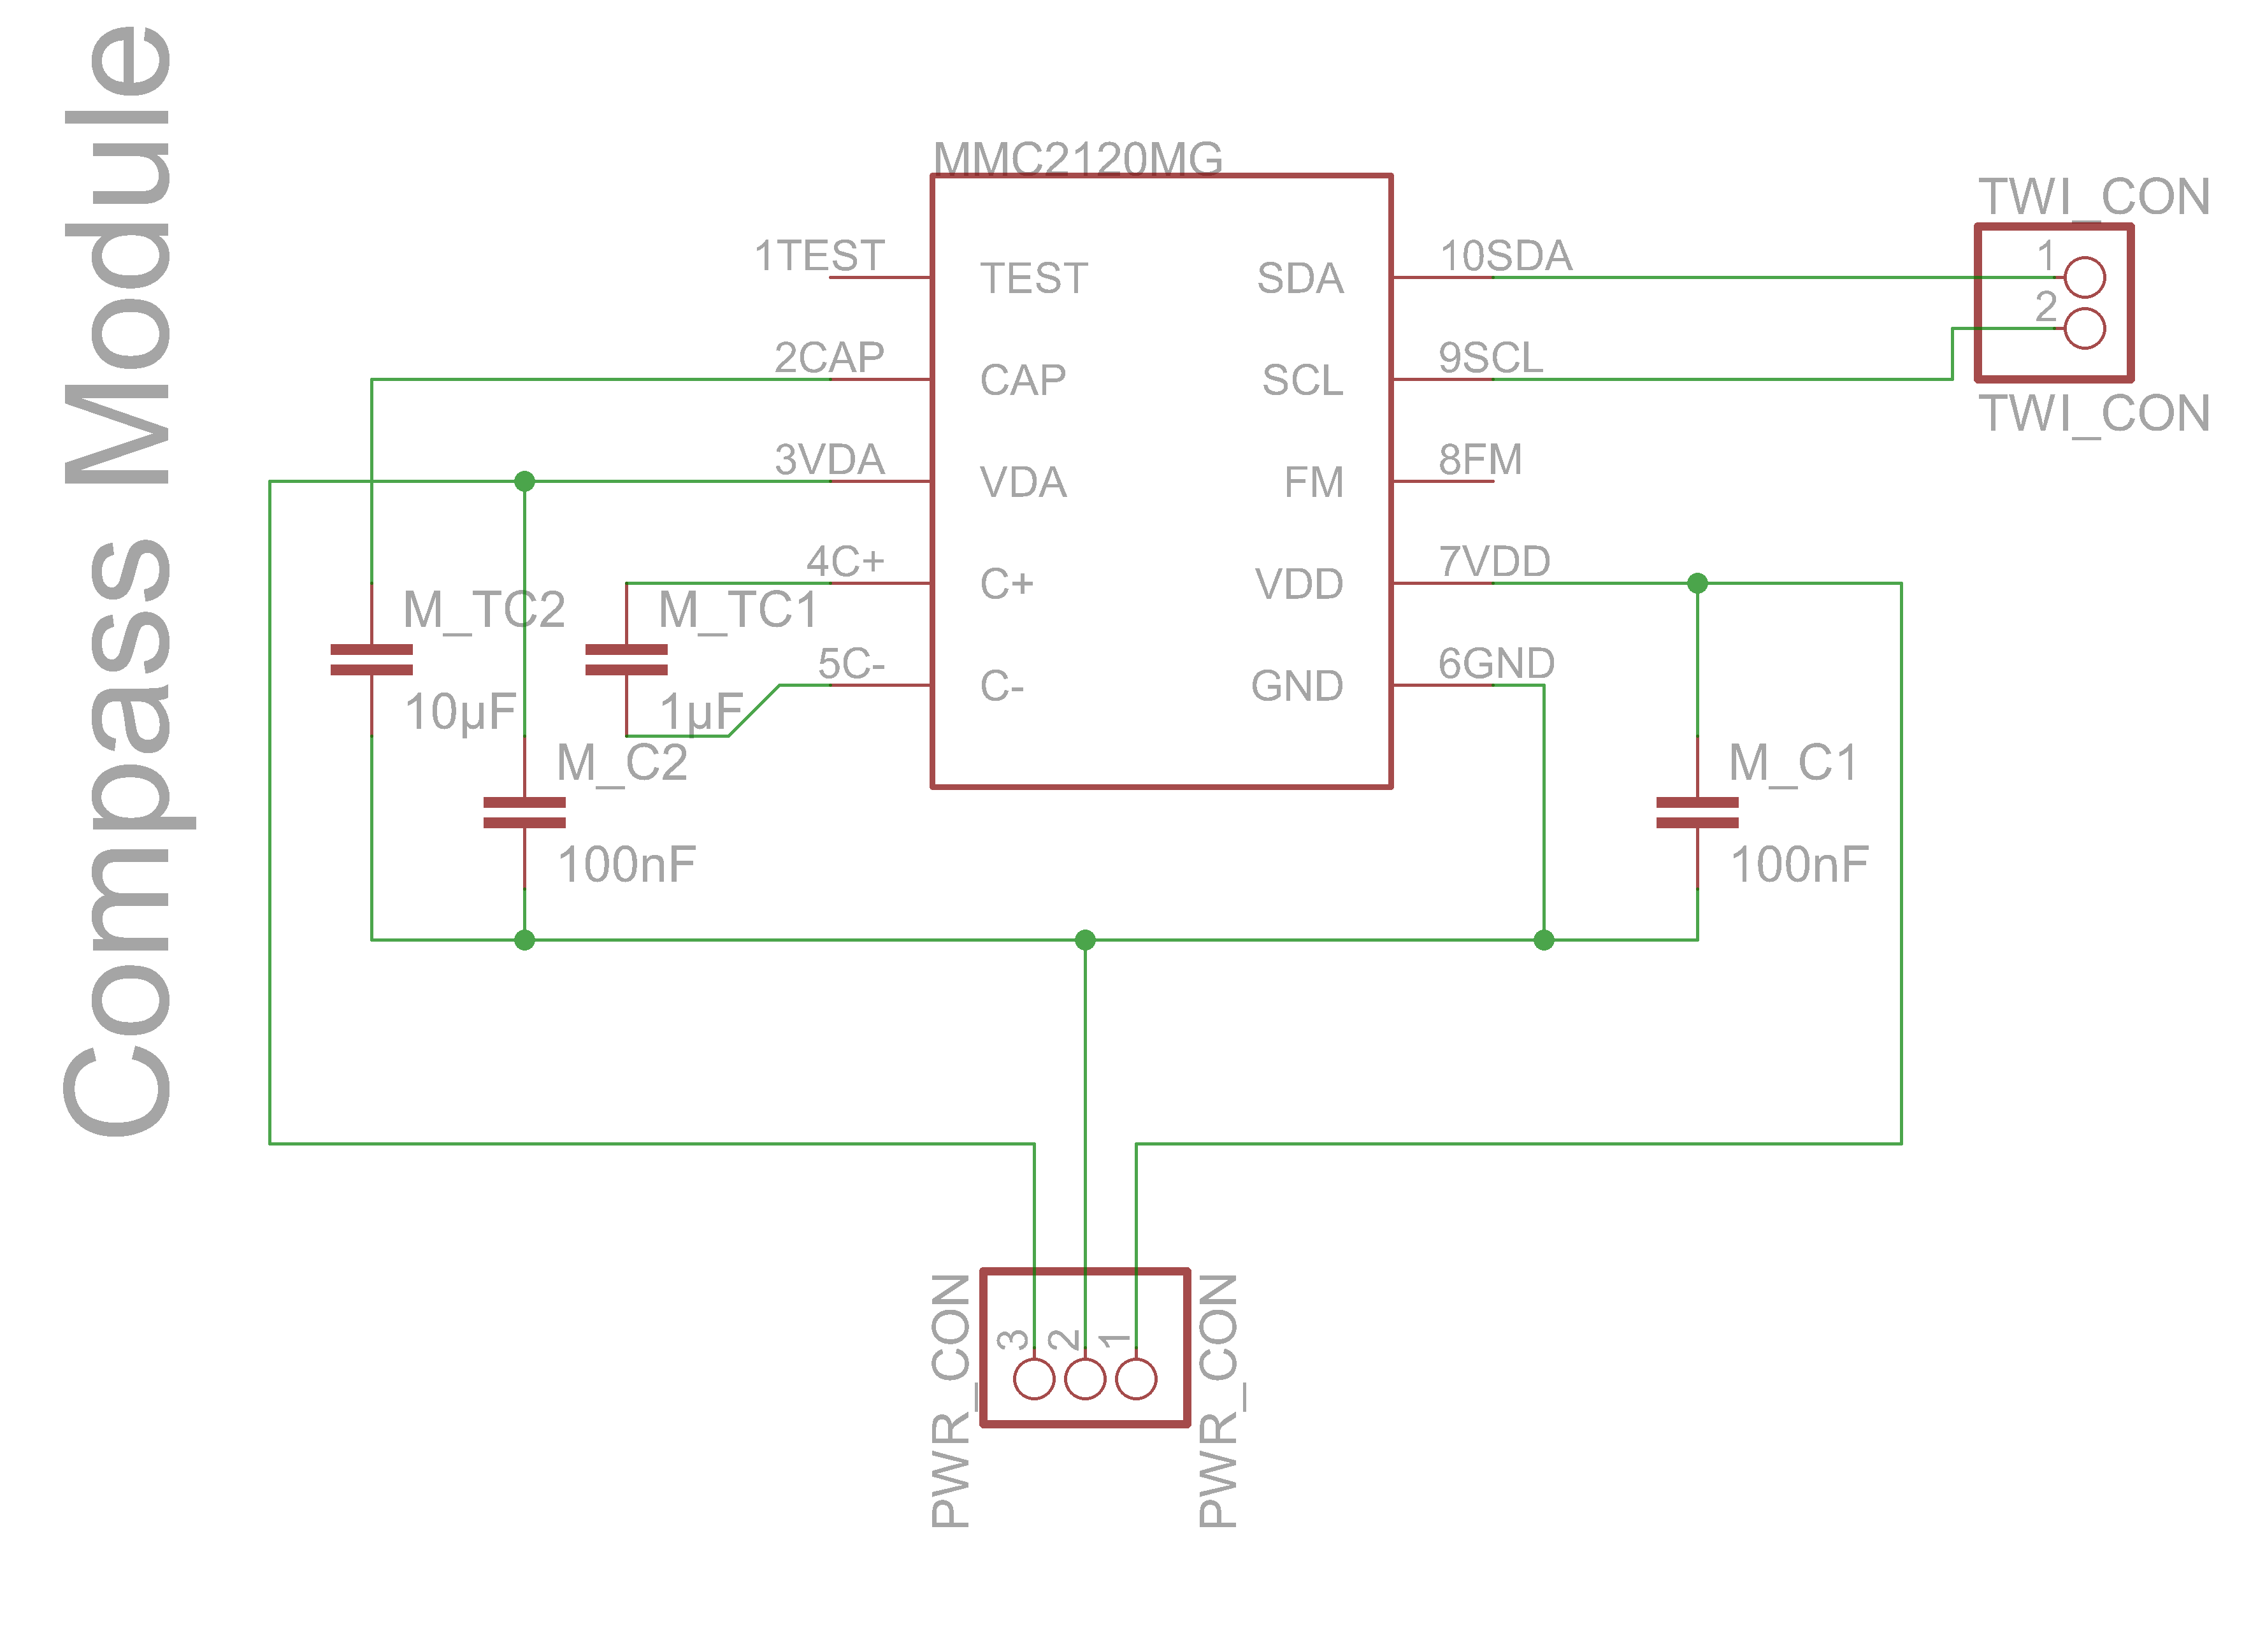
\includegraphics[height=100mm]{../images/ch04/mmc2120mgsch.png}
 \caption{Schemat modułu kompasu}
 \label{fig:MMC2120Sch}
\end{figure}

\begin{figure}[!ht]
 \centering
 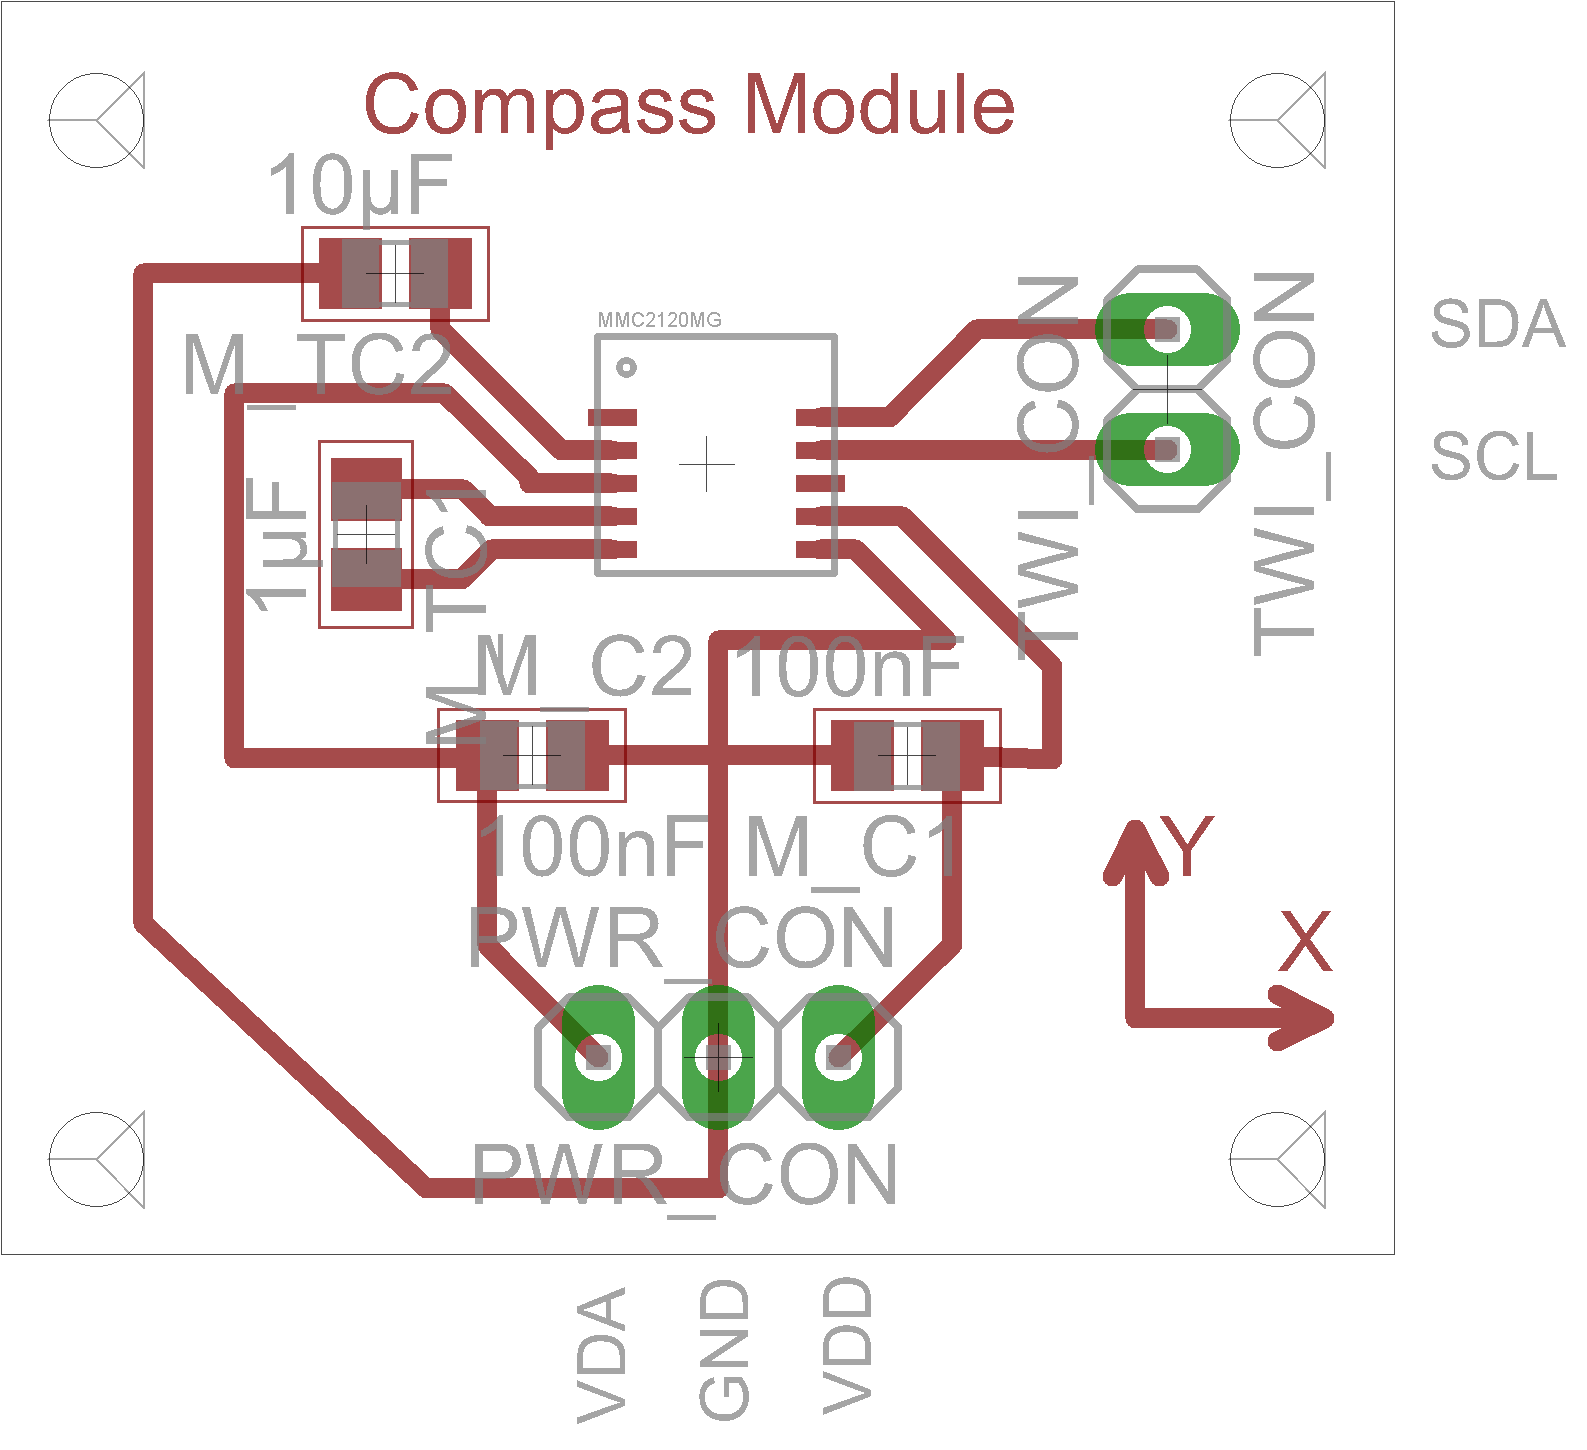
\includegraphics[height=50mm]{../images/ch04/mmc2120mgpcb.png}
 \caption{Projekt płytki kompasu elektronicznego}
 \label{fig:MMC2120Pcb}
\end{figure}

\begin{table}[hb]
  \rowcolors{2}{white}{gray!20}
  \centering
  \caption{Opis wyprowadzeń modułu kompasu}
  \begin{tabular}{ | c | c | c | p{1.75cm} |} \hline
    Nazwa & Typ & Opis \\ \hline
    VDA & Zasilanie & Napięcie zasilania $3.3V$ \\
    GND & Zasilanie & Masa \\
    SCL & Wejście & Zegar sterujący $I^{2}C$ \\
    SDA & We / Wy & Szyna do przesyłania danych $I^{2}C$ \\
    VDD & Zasilanie & Napięcie zasilania szyny danych $3.3V$ \\ \hline
  \end{tabular}
  \label{tab:MMC2120ModOut}
\end{table}

\begin{figure}[!ht]
 \centering
 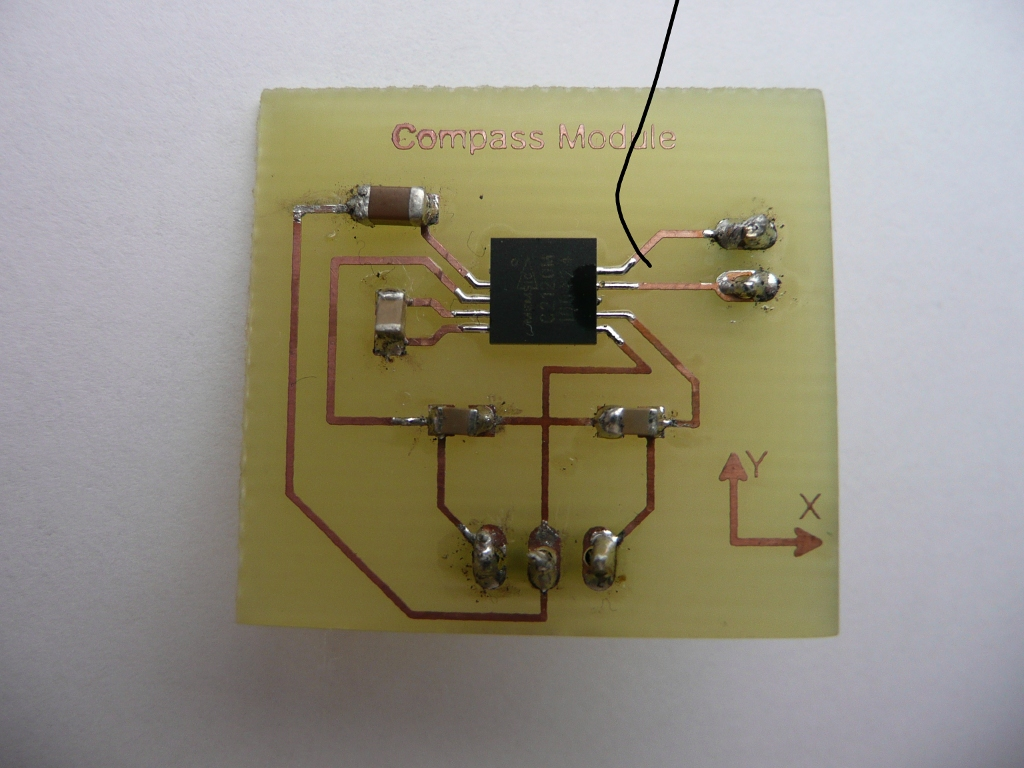
\includegraphics[height=50mm]{../images/ch04/compassmodule.jpg}
 \caption{Gotowy moduł kompasu}
 \label{fig:L3G4200DModule}
\end{figure}

\subsection{Nieudana próba zastosowania}
Docelowo moduł kompasu miał być wykorzystywany jako element Inercjalnego Systemu Nawigacji w celu określania kierunku w którym robot się przemieszcza. Zasada działania miała być prosta. Robot miał zapamiętywać aktualny azymut z jakim się poruszał będąc na rekach operatora. Następnie po postawieniu na podłożu miał odtwarzać tor ruchu obracając wszystkie zapamiętane azymuty o $180\circ$. 

\begin{figure}[!ht]
 \centering
 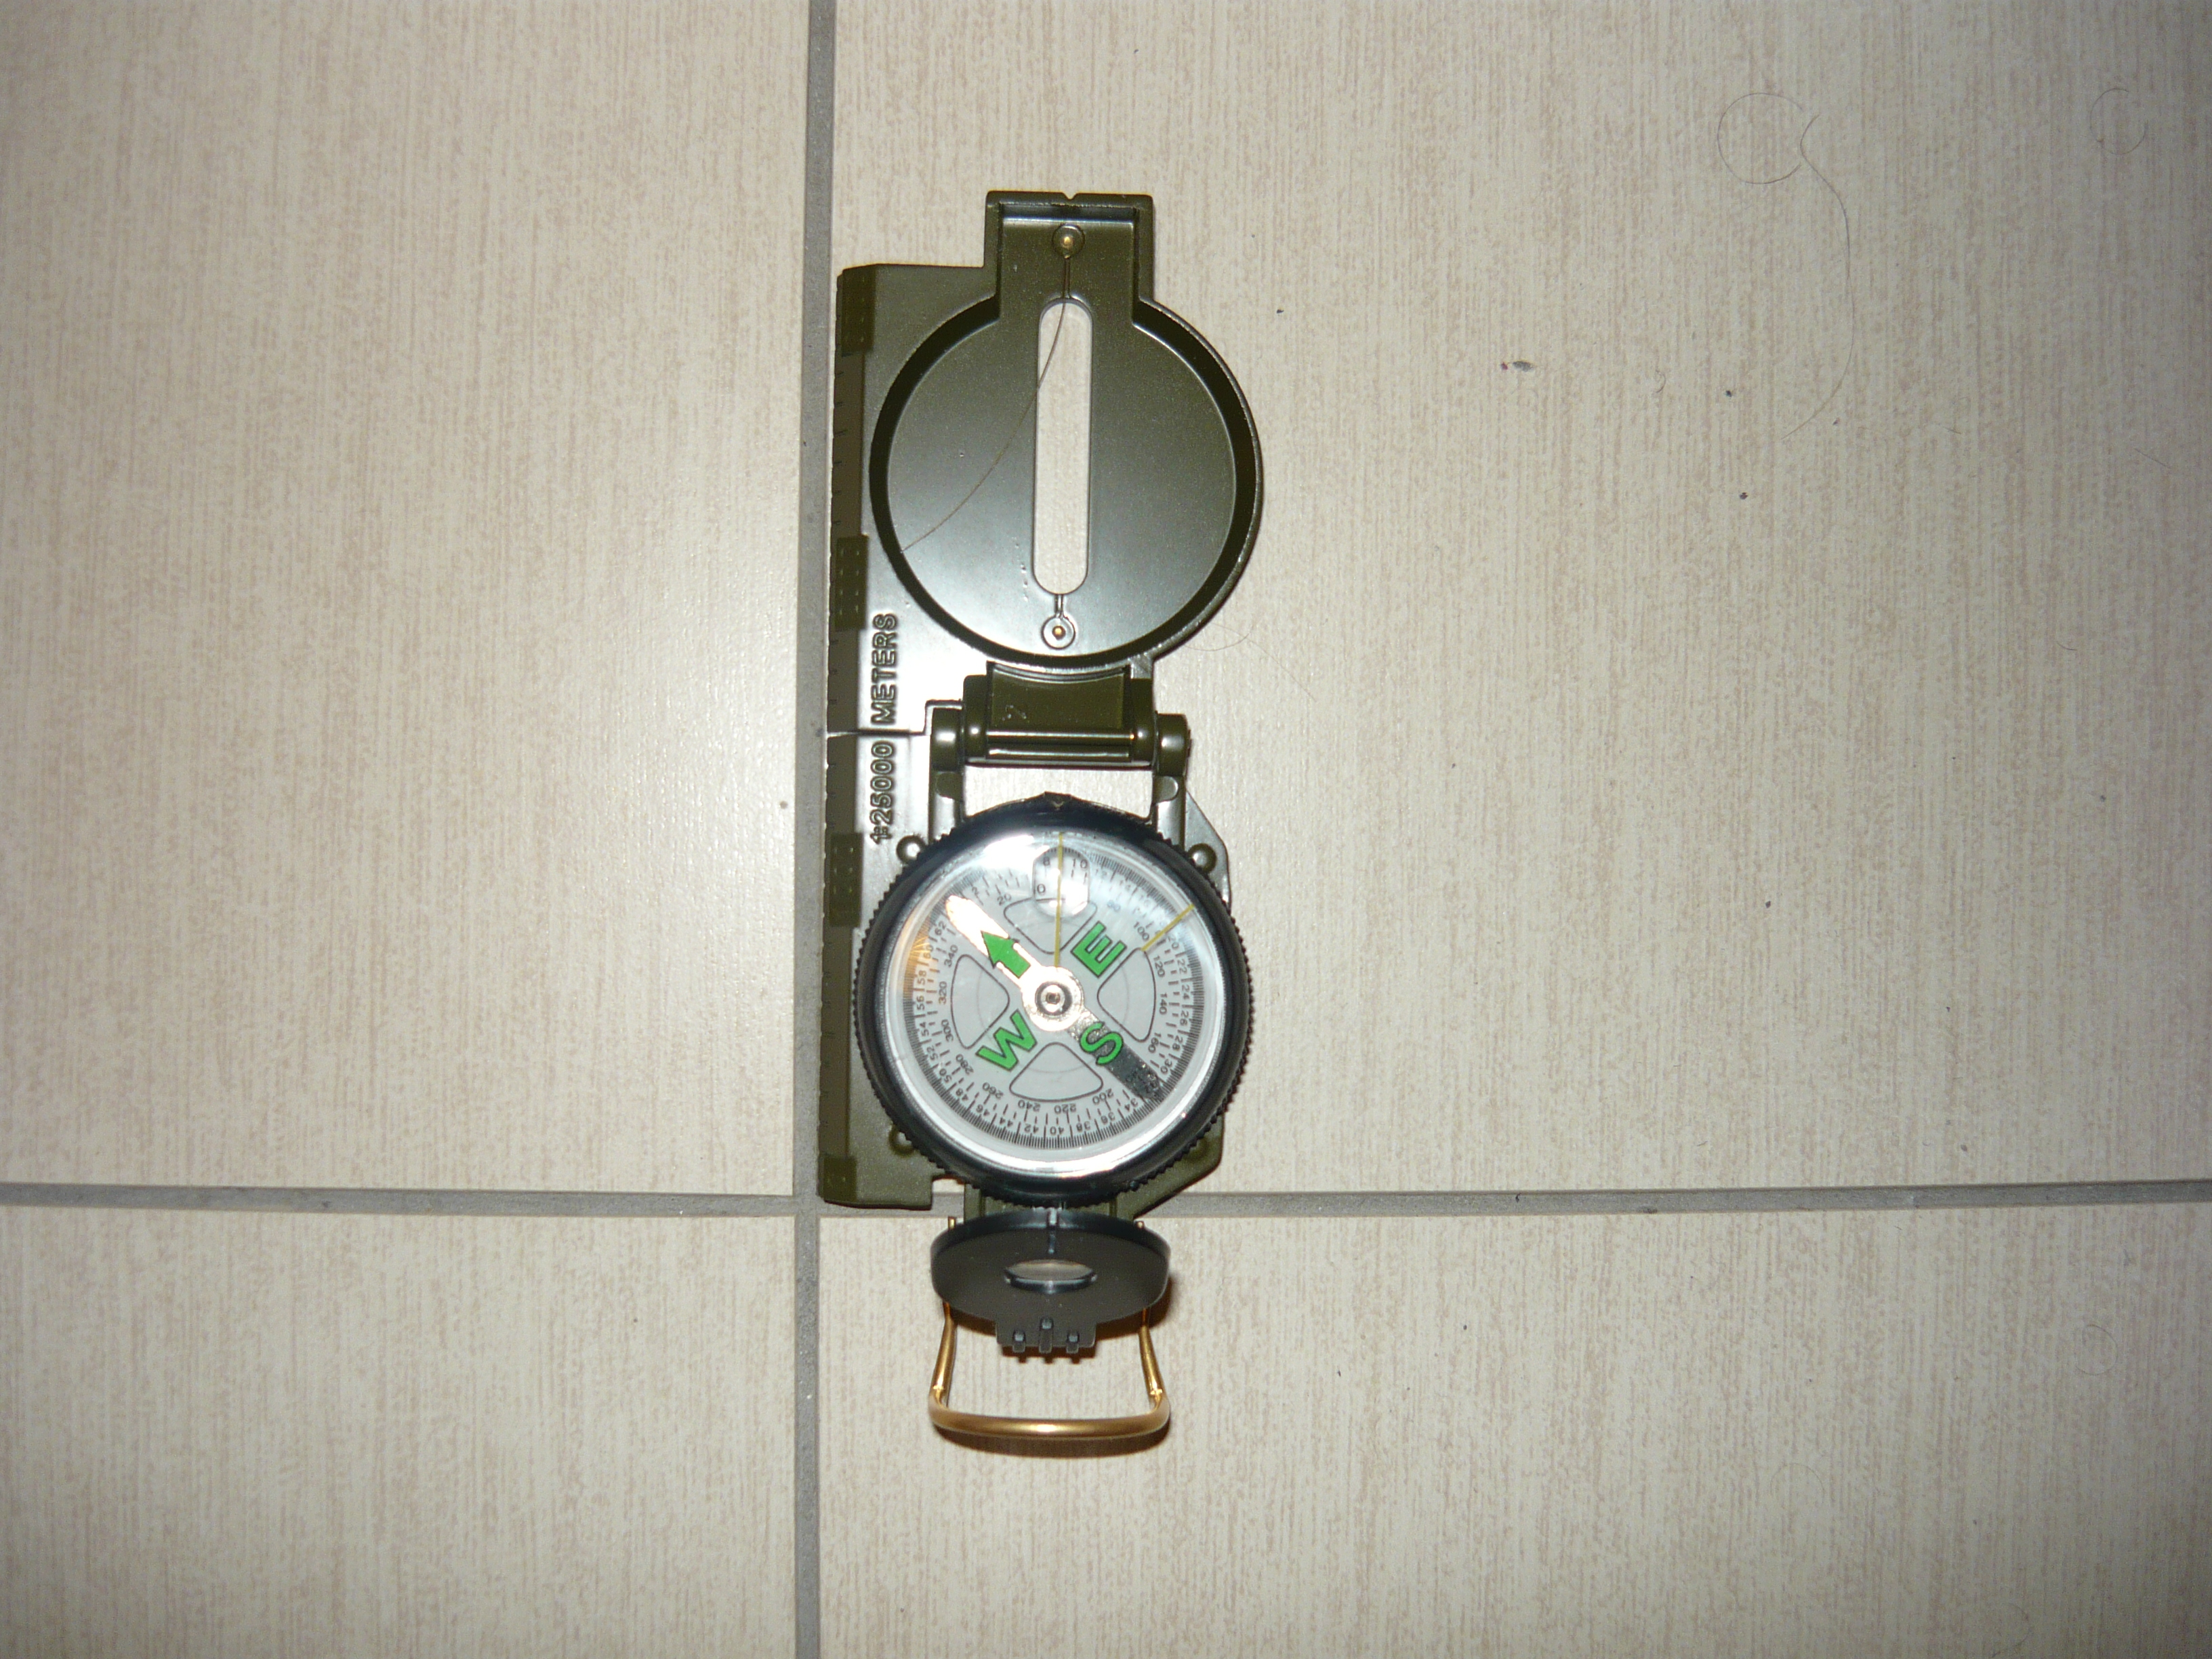
\includegraphics[height=75mm]{../images/ch04/compass01.jpg}
 \caption{Busola w położeniu początkowym}
 \label{fig:Busola1}
\end{figure}

\begin{figure}[!ht]
 \centering
 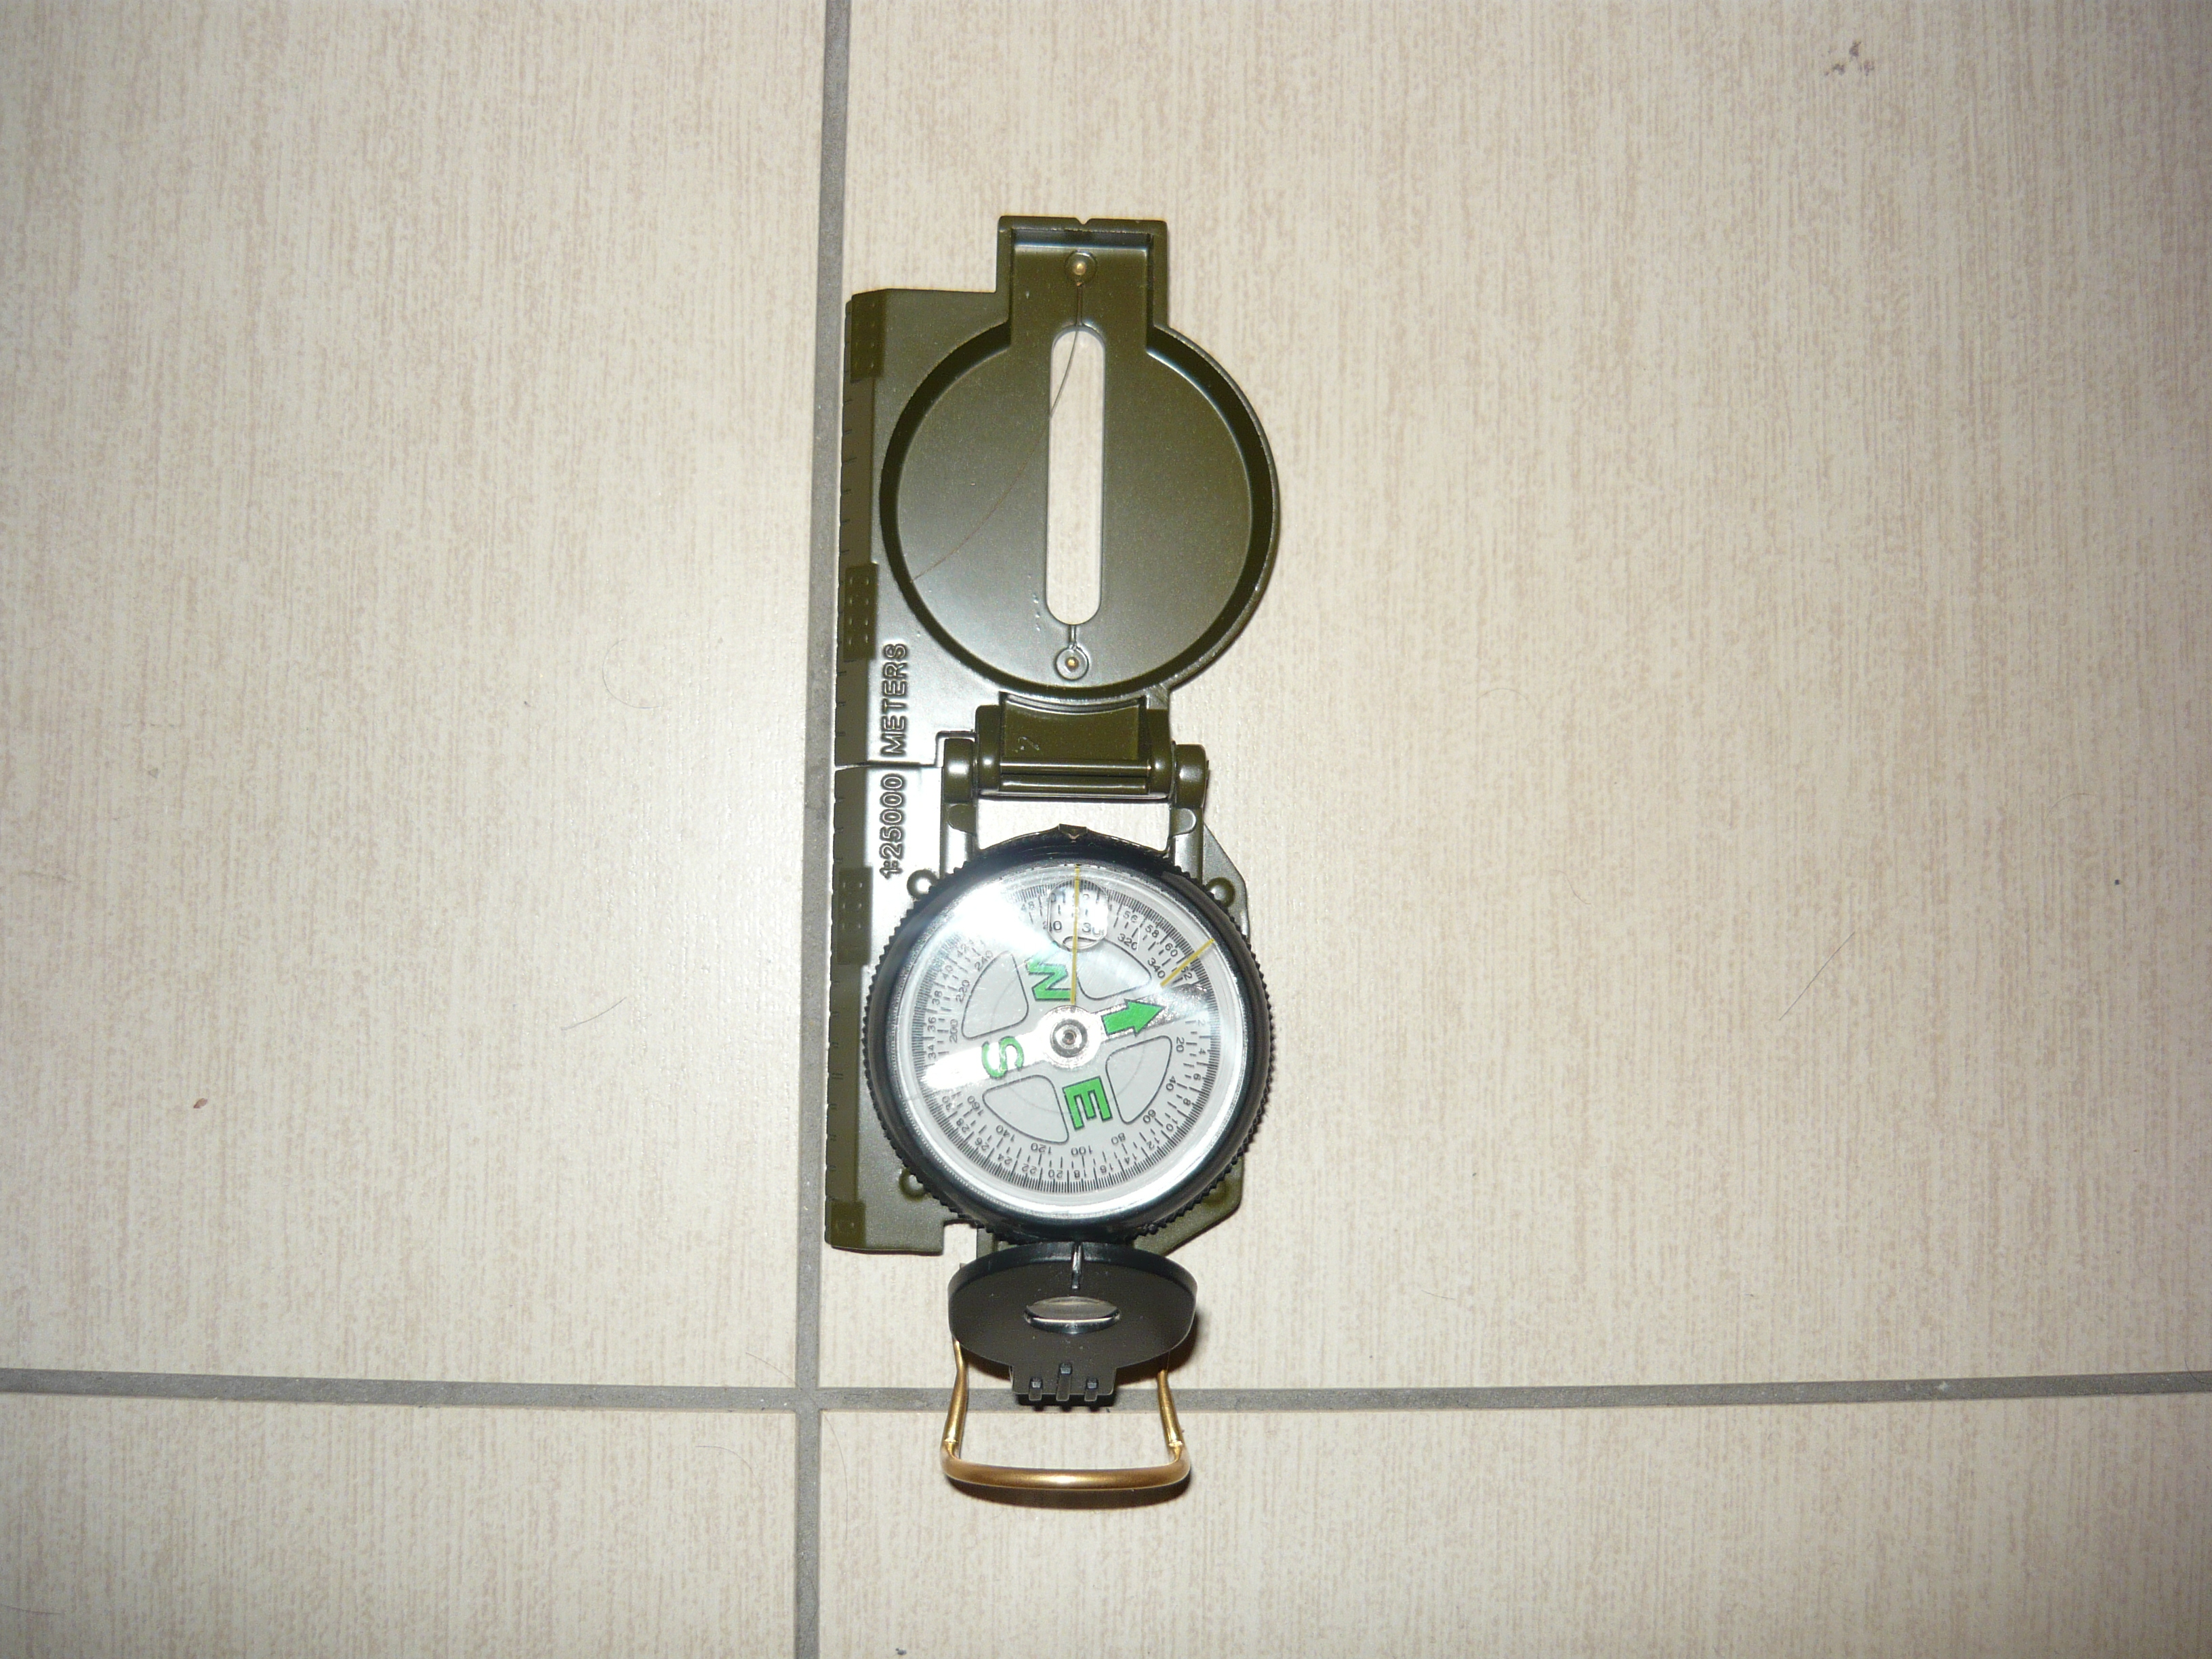
\includegraphics[height=75mm]{../images/ch04/compass02.jpg}
 \caption{Busola przesunięta równolegle o 25 cm,}
 \label{fig:Busola2}
\end{figure}

Niestety wykonane testy pokazały, iż nie jest możliwe wykorzystanie kompasu w celu określenia azymutu robota poruszającego się po podłodze budynku. Jest to spowodowane stosowaniem metalowych prętów zbrojeniowych w stropach budynków, które zakłócają pracę kompasu. Testy zostały wykonane zarówno przy pomocy modułu elektronicznego kompasu jak i tradycyjnej wojskowej busoli. Rysunki \ref{fig:Busola1} oraz \ref{fig:Busola2} przedstawiają odchylenie azymutów wyznaczonych na podłodze budynku. Busola przedstawiona na zdjęciach została przesunięta równolegle o 25 cm w prawo. Wskazywany kierunek północy zmienił się o ponad $90^{\circ}$. Jak widać przy tak dużych wahaniach nie jest możliwe wykorzystanie magnetometru jako elementu jednoznacznie określającego kierunek w którym robot ma się poruszać. Po wielu nieudanych próbach wyeliminowania zakłóceń moduł kompasu został zastąpiony modułem żyroskopu.

% http://www.iemw.tuwien.ac.at/publication/workshop0600/Hauser.html
\section{Czujnik odległości}
Bardzo popularnym rozwiązaniem problemu omijania przeszkód jest wykorzystanie
czujników ultradźwiękowych. Dane pomiarowe pobrane w pierwszym kroku z sonaru
wykorzystywane są to stworzenia lokalnej reprezentacji otoczenia pozwalającej na
późniejsze sterowanie robotem\cite{ObstaclesAvoidanceIR}. Dla tak zdefiniowanego
problemu możemy wyróżnić dwa rodzaje reprezentacji środowiska. Pierwszy rodzaj
reprezentacji opiera się o siatkę dzięki której środowisko podzielone jest na
skończoną liczbę komórek które mogą posiadać stan świadczący o pustej przestrzeni
lub obecności przeszkody w danej komórce. Drugim sposobem reprezentacji jest
przedstawienie otoczenia za pomocą zbioru właściwości takich jak punkty, linie
oraz płaszczyzny. Wybór sposobu reprezentacji jest z reguły podyktowany
rodzajem problemu jaki stawiany jest przed robotem mobilnym.

Innym rodzajem czujników bardzo dobrze sprawdzających się w rozwiązywaniu
problemu omijania przeszkód są dalmierze oparte o czujnik podczerwieni. Często
zdarza się, iż dalmierze IR\footnote{IR (ang. infrared) - skrótowe oznaczenie
urządzeń wykorzystujących podczerwień do swojego działania} są wybierane ze
względu na ich bardzo krótki czas odpowiedzi w porównaniu do czujników
ultradźwiękowych. Niestety jakość pomiaru w przypadku
czujników podczerwieni jest w dużym stopniu zależna od współczynnika odbicia
powierzchni przeszkody, jak również odległości od przeszkody oraz położenia
nadajnika i odbiornika w~stosunku do powierzchni przeszkody. Zdarza się więc, że
brak precyzyjnych danych o~lokalizacji przeszkody i jej właściwościach
wykluczają dalmierze IR z niektórych zastosowań. Jednakże szeroka dostępność
tego typu urządzeń oraz łatwość ich wykorzystania spowodowała, że są one
najczęściej stosowane w robotach zajmujących się podążaniem za~ścianą czy
omijaniem i liczeniem przeszkód.

\begin{figure}[h!]
 \centering
 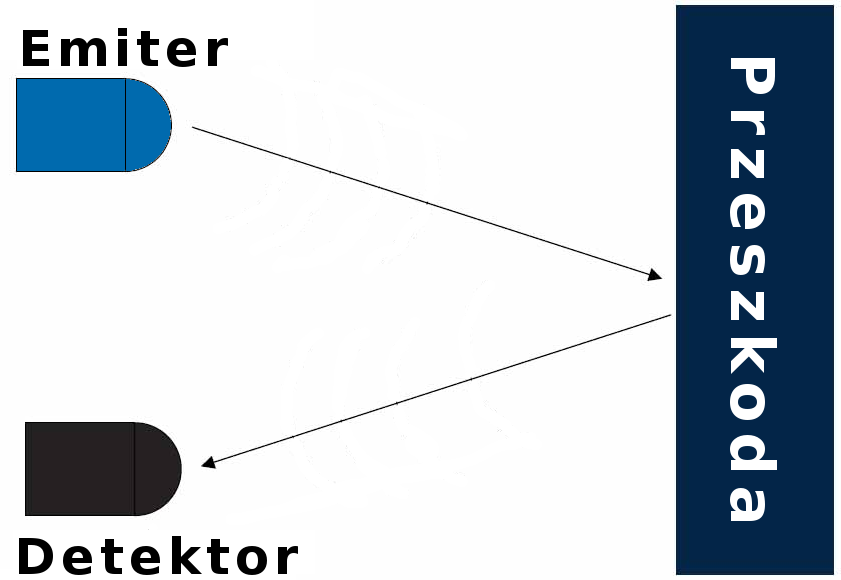
\includegraphics[height=62mm]{../images/ch04/ir_sensor.png}
 \caption{Zasada działania dalmierza wykorzystującego podczerwień}
 \label{fig:IRSensors}
\end{figure}

Typowy dalmierz IR składa się z dwóch elementów. Pierwszym z nich jest dioda
emitująca promieniowanie podczerwone, natomiast drugim elementem jest detektor
najczęściej fotodioda lub fototranzystor. 
Zasada działania tak zbudowanego
czujnika odległości opiera się o zjawisko odbicia. Światło wyemitowane przez
emiter odbija się od przeszkody i trafia do detektora. Niestety pomiar tego
rodzaju jest niezwykle wrażliwy na zmiany w oświetleniu oraz rodzaj i kształt
napotkanej przeszkody.
 
\subsection{Algorytm omijania przeszkód}
Algorytm sterujący ruchami robota bazuje w całości na danych pomiarowych
otrzymanych z czujników robota. Opisane podejście jest adaptacją metodologii
opisanej w ramach pracy ,,Obstacles Avoidance Method for an Autonomous Mobile
Robot'' \cite{ObstaclesAvoidanceIR}. Zaproponowane rozwiązanie bazuje na prostej
maszynie stanów w której przejścia pomiędzy kolejnymi stanami odbywają się
poprzez zmianę poziomów na czujnikach odległości. Autorzy proponują podłączenie
do robota dwóch dalmierzy jednego po lewej (LS), a drugiego po prawej stronie
(RS) robota w taki sposób aby przed robotem nie było martwego punktu. Sposób
montażu czujników został przedstawiony na rysunku poniżej.

\begin{figure}[h!]
 \centering
 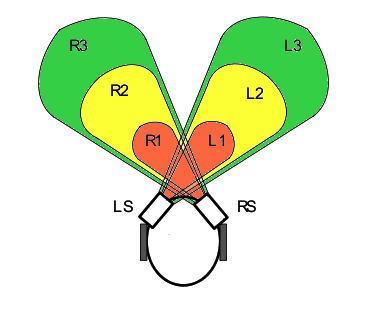
\includegraphics[height=70mm]{../images/ch04/ir_sensor_position.png}
 \caption{Sposób montażu czujników podczerwieni na robocie \cite{ObstaclesAvoidanceIR}}
 \label{fig:IRSensorPosition}
\end{figure}

Każdy z czujników składa się z nadajnika i odbiornika podczerwieni, a ich
przedział czułości, zgodnie z zaleceniami autorów, podzielony został na trzy
poziomy oznaczone symbolami L1, L2, L3 dla czujnika lewego i odpowiednio R1, R2,
R3 dla czujnika prawego. Istotne jest aby kolejne poziomy ułożone były w porządku
rosnącym, a przerwa pomiędzy kolejnymi była na tyle szeroka, aby zminimalizować
wpływ niedokładności pomiaru odległości. W chwili gdy robot znajduje się w ruchu
na każdym z czujników jesteśmy w stanie odczytać wartość odległości od
przeszkody. Dzięki takiej informacji możemy jednoznacznie kontrolować zachowanie
robota w zależności od poziomu jaki w danej chwili ustalił się na poszczególnych
dalmierzach. 

Opierając się na takich założeniach, jeżeli oba czujniki nie
wykrywają na swojej drodze przeszkody to robot porusza się z maksymalną możliwą
prędkością. Gdy jeden z czujników wykryje obecność przeszkody na poziomie  L3
lub/i R3 prędkość poruszania się robota zostanie zmniejszona o połowę. Gdy
przeszkoda znajdzie się w odległości poziomu L2 lub/i R2 prędkość z jaką porusza
się robot zostanie ustalana na 1/4 prędkości maksymalnej. Jeżeli natomiast
przeszkoda zostanie wykryta na poziomie L1 lub/i R1 robot skręci w prawo lub lewo
w zależności od położenia przeszkody i wyznaczonego celu.

Na poniższym rysunku zaprezentowane zostały cztery najbardziej typowe ze
wszystkich z możliwych sytuacji oraz definicja manewru jaki robot
podejmie, aby skutecznie ominąć napotkaną przeszkodę. 

\begin{figure}[h!]
 \centering
 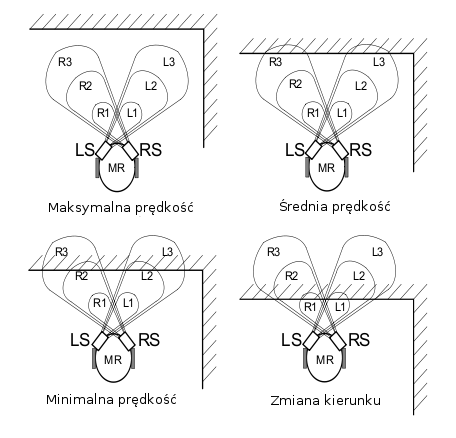
\includegraphics[height=140mm]{../images/ch04/obs_avoid_algorithm.png}
 \caption{Przykładowe sytuacje i definicja reakcji robota}
 \label{fig:IRTestCases}
\end{figure}

Uogólniając zasadę działania algorytmu, robot dostosowuje swoją prędkość na
podstawie aktualnej odległości od przeszkody odczytanej z czujników odległości.
W chwili gdy robot znajdzie się bezpośrednio przed przeszkodą skręci on w prawo
lub lewo aby ją ominąć. Kąt o jaki wykonany zostanie zakręt zależy od tego na
którym czujniku przeszkoda została wykryta oraz aktualnego celu do którego robot
zmierza. Szczegółowy opis poszczególnych możliwych sytuacji oraz rodzaj akcji
podejmowanej przez robota jest przedstawiony w tabeli na następnej stronie. 

Podane w tabeli wartości mają charakter orientacyjny i w gdy robot ma
wyznaczony cel do którego zmierza kierunki skrętu mogą w niektórych przypadkach
ulec zmianie. Mogą również pojawić się dodatkowe zmiany kierunku jazdy umożliwiające
powrócenie na ścieżkę do wyznaczonego punktu docelowego.

W pierwszych sześciu kolumnach tabeli prezentowany jest stan ustalony na poszczególnych
poziomach odległości z podziałem na czujnik prawy i lewy. Jedynka w odpowiedniej
kolumnie oznacza obecność przeszkody w danym przedziale odległości, natomiast
zerem oznaczany jest brak przeszkody. W ostatniej kolumnie prezentowana jest
akcja jaką podejmie robot po wykryciu danej konfiguracji stanów.

\begin{table}[hb]
\rowcolors{2}{white}{gray!20}
\centering
\caption{Zachowanie robota w zależności od stanu wykrywanego na czujnikach odległości}
   	\begin{tabular}{ | c | c | c | c | c | c | p{4.75cm} |} \hline
   		R3 & L3 & R2 & L2 & R1 & L1 & Akcja robota \\ \hline
   		0  & 0  & 0  & 0  & 0  & 0  & Maksymalna prędkość\\ \hline
   		0  & 1  & 0  & 0  & 0  & 0  & Średnia prędkość \\ \hline
   		0  & 1  & 0  & 1  & 0  & 0  & Minimalna prędkość \\ \hline
   		0  & 1  & 0  & 1  & 0  & 1  & Skręt w lewo o $45\,^{\circ}$ \\ \hline 
   		1  & 0  & 0  & 0  & 0  & 0  & Średnia prędkość \\ \hline
   		1  & 0  & 1  & 0  & 0  & 0  & Minimalna prędkość \\ \hline
   		1  & 0  & 1  & 0  & 1  & 0  & Skręt w prawo o $45\,^{\circ}$  \\ \hline
   		1  & 1  & 0  & 0  & 0  & 0  & Średnia prędkość \\ \hline
   		1  & 1  & 1  & 0  & 0  & 0  & Minimalna prędkość \\ \hline
   		1  & 1  & 1  & 0  & 1  & 0  & Skręt w prawo o $45\,^{\circ}$ \\ \hline
   		1  & 1  & 0  & 1  & 0  & 0  & Minimalna prędkość \\ \hline
   		1  & 1  & 0  & 1  & 0  & 1  & Skręt w lewo o $45\,^{\circ}$ \\ \hline 
   		1  & 1  & 1  & 1  & 0  & 0  & Minimalna prędkość \\ \hline 
   		1  & 1  & 1  & 1  & 0  & 1  & Skręt w lewo o $45\,^{\circ}$ \\ \hline 
   		1  & 1  & 1  & 1  & 1  & 0  & Skręt w prawo o $45\,^{\circ}$ \\ \hline 
   		1  & 1  & 1  & 1  & 1  & 1  & Skręt w lewo o $90\,^{\circ}$ \\ \hline
   	\end{tabular}
\label{ObstacleAvoidTable}
\end{table}
\newpage
\subsection{Implementacja}
W zrealizowanej w ramach pracy magisterskiej implementacji robot, Dark Explorer,
wyposażony został w dwa dalmierze Sharp GP2D12 o efektywnym zasięgu od 10 do 80
cm. Każdy z~dalmierzy wyposażony jest w nadajnik i odbiornik IR. Czujnik
GP2D12 samodzielnie dokonuje pomiaru odległości i zwraca go w postaci sygnału
analogowego. Dlatego też, robot wykorzystuje konwerter analogowo-cyfrowy do
przetwarzania wyniku pomiaru otrzymanego z czujnika. Wartość napięcia otrzymana
na wyjściu z konwertera jest za pomocą równania, otrzymanego na podstawie
charakterystyki wyjściowej dalmierza, zamieniana na odległość czujnika od
przeszkody. Na zdjęciu poniżej zaznaczone zostały poszczególne elementy składowe
czujnika oraz kolejne wyprowadzenia.

\begin{figure}[hb]
 \centering
 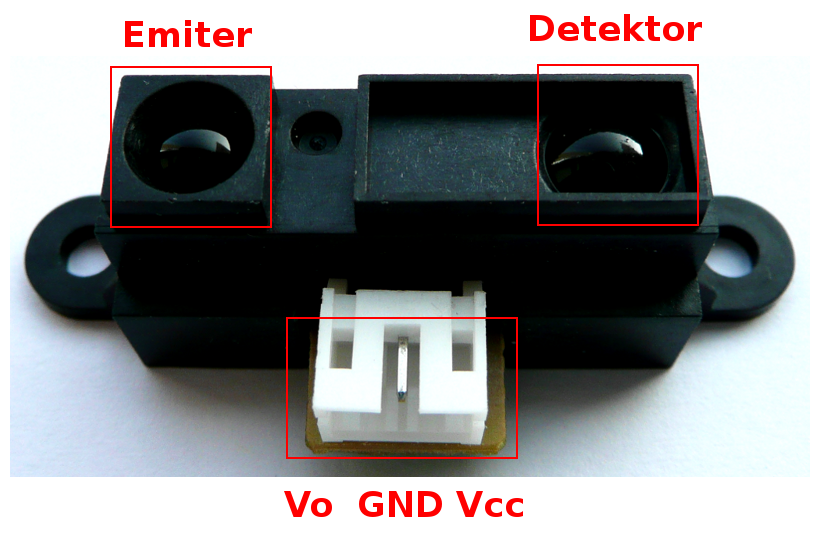
\includegraphics[width=100mm]{../images/ch04/real_gp2d12_view.png}
 \caption{Budowa czujnika GP2D12 wraz z wyporowadzeniami}
 \label{fig:SharpGP2D12}
\end{figure}

Zastosowany czujnik odległości został wyposażony w unowocześniony sposób
dokonywania pomiarów odległości. Użyty dalmierz wykorzystuje triangulację oraz
małą liniową matrycę CCD aby obliczyć odległość od przeszkody w polu
widzenia sensora\cite{website:acroname-robotics}. Podstawową zasadą działania
nowego systemu pomiaru odległości jest wysłanie impulsu światła podczerwonego który po odbiciu od przeszkody wraca
do detektora i tworzy trójkąt pomiędzy emiterem, detektorem a przeszkodą. Kąty w
tym trójkącie zmieniają się razem z odległością od przeszkody, co zostało
zaprezentowane na rysunku \ref{fig:SharpGP2D12_opertaion_theory}.

Kluczem do poprawnego działania takiego rozwiązania jest soczewka która dba o to, aby
odbite światło trafiało na odpowiednie pole matrycy CCD w zależności od wartości
kątów w opisanym powyżej trójkącie. Dzięki takiej budowie soczewki, czujnik na
podstawie danych z matrycy CCD może określić kąt pod jakim światło odbite
wróciło, a dzięki temu jest w stanie obliczyć aktualną odległość od przeszkody.
Zastosowana w dalmierzu metoda pomiaru odległości jest niemal całkowicie odporna
na zakłócenia spowodowane światłem zewnętrznym. Dodatkowo eliminuje błędy
pomiarowe związane z kolorem powierzchni przeszkody. Dzięki zastosowaniu takiego
podejścia możliwe jest wykrycie całkowicie czarnej ściany w całości oświetlonej
przez intensywne światło słoneczne, co w przypadku starszych dalmierzy
praktycznie nie jest możliwe.

\begin{figure}[h!]
 \centering
 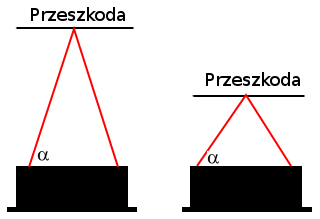
\includegraphics[width=100mm]{../images/ch04/gp2d12_operation_theory.png}
 \caption{Zasada przeprowadzania pomiaru przez czujnik GP2D12}
 \label{fig:SharpGP2D12_opertaion_theory}
\end{figure} 

Zgodnie z założeniami algorytmu obszar zasięgu czujników został podzielony na
trzy poziomy. Poziom trzeci zostały wyznaczony w odległości 50 cm, drugi poziom
wyznaczony został w odległości 25 cm, a poziom pierwszy wyznaczony został w
odległości 12 cm od przeszkody. Program zarządzający działaniem robota odczytuje
kolejno dane o odległości otrzymane z czujnika prawego i lewego i kontroluje
zachowanie robota zgodnie z zasadami przedstawionymi w tabeli
\ref{ObstacleAvoidTable}. Z praktycznego punktu widzenia implementacja tego
rodzaju algorytmu sprowadza się do stworzenia tablicy w której przechowywane są
prędkości poruszania się każdego z czterech kół z uwzględnieniem lokalizacji
czujnika oraz progu odległości w jakim znajduje się przeszkoda.

Aby móc praktycznie wykorzystać dane analogowe uzyskane z dalmierza wykorzystany
został wbudowany w robota przetwornik analogowo-cyfrowy (ADC). Sposób obsługi
przetwornika analogowo-cyfrowego, na potrzeby omijania przeszkód, został
zrealizowany w oparciu o dokumentację i przykłady zawarte w książce J. Augustyna
pt. ,,Projektowanie systemów wbudowanych na przykładzie rodziny SAM7S z rdzeniem
ARM7TDMI''. Zgodnie ze specyfikacją, przetwornik, wbudowany w procesor SAM7S
pozwala na przetwarzanie napięcia w granicach od 0V do napięcia referencyjnego
które w przypadku robota Dark Explorer jest równe napięciu zasilania procesora
tj. 3.3V. Aby uzyskać jak najdokładniejszy wynik pomiaru
przetwornik został skonfigurowany do pracy z rozdzielczością 10-bitową. Wydłuża to czas potrzebny na
konwersję danych jednakże przy prędkościach z jakimi robot się porusza nie ma to
większego wpływu na jakość działania aplikacji gdyż wykorzystany przetwornik
ADC mierzy i zwraca wartość chwilową napięcia\cite{JAugustyn}.

W trakcie działania aplikacji uruchamiany jest proces konwersji na kanałach do
których podłączone są czujniki odległości, a następnie aplikacja oczekuje na
wywołanie przerwania związanego z wpisaniem wartości na temat napięcia do
odpowiednich rejestrów. Po otrzymaniu wartości napięcia widocznego na wyjściu z
dalmierzy, obliczana jest odległość w jakiej znajduje się przeszkoda. Ze względu
na zastosowaną metodę pomiarową napięcie wyjściowe z czujników odległości nie ma
charakterystyki liniowej. Jest to związane obliczeniami trygonometrycznymi
wykonywanymi w celu wyznaczenia odległości od przeszkody. 
W tym celu,
udostępniona w ramach dokumentacji czujnika\cite{GP2D12DataSheet} charakterystyka
wyjściowa, posłużyła do wyznaczenia progów napięcia dla zdefiniowanych przez
algorytm progów odległości.
% W tym celu,
% udostępniona w ramach dokumentacji czujnika\cite{GP2D12DataSheet} charakterystyka
% wyjściowa, posłużyła do wyznaczenia równania pozwalającego z zadowalającą
% dokładnością wyznaczyć odległość od przeszkody. 
% W wyniku dopasowania otrzymano
% równanie postaci.
% \begin{equation}
% y=\frac{a+bx}{1+cx+dx^2}
% \end{equation}
% Powyższe równanie nie odzwierciedla w pełni charakterystyki czujnika, ale w
% bardzo dobry sposób przybliża ją w przedziale wymaganym do prawidłowej
% implementacji algorytmu. Posiadając tak przygotowane dane zaimplementowanie
% reszty algorytmu nie stanowiło już większej trudności. 

W ramach testów przeprowadzono kilka symulacji działania implementacji dla
różnych pozycji startowych przy zbliżaniu się robota to brzegu przeszkody. Już
pierwsze testy wykazały, że gdy robot porusza się prostopadle do płaszczyzny
ściany algorytm działa bardzo dobrze, jednakże w przypadku gdy ruch ten nie jest
prostopadły w niektórych przypadkach pojawiają się problemy z działaniem
algorytmu. Wspomniane problemy związane są z w niektórych przypadkach z
odbieraniem przez dalmierz dodatkowych sygnałów wysłanych z sąsiedniego czujnika.
Rozwiązaniem takiego problemu mogłoby być zastosowanie czujników z kodowaniem
sygnału. Co więcej zasada działania dalmierzy IR nie pozwala na wykrycie małych i
wąskich obiektów stawianych na drodze robota. Dodatkowym problemem jest
nieliniowość charakterystyki czujnika która przy odległości mniejszej od 10cm
wskazuje napięcia które mogą być mylnie zinterpretowane.

\section{Wyświetlacz LCD}
\label{sec:lcd}
Do sygnalizacji wykonywanych czynności oraz polepszenia komunikacji pomiędzy
człowiekiem a robotem został wykorzystany wyświetlacz LCD. Użyty model to
wyświetlacz LCD 2x16, ze złączem pasującym do płyt systemu EVBXXX, z
podświetleniem biało-niebieskim. Element ten został wybrany ze względu na
stosunkowo niską cenę oraz możliwość podłączenia do płyty ewaluacyjnej EVBsam7s
wykorzystywanej podczas rozwoju robota.

Na wyświetlaczu pokazywane są czynności aktualnie wykonywane przez robota oraz
informacje pobierane z czujników zamontowanych na nim. Przykładowe komunikaty
pokazywane przez Dark Explorera mówią o: aktualnej temperaturze, ilości kroków
które wykonał użytkownik, kierunku w jakim podąża.

\begin{figure}[!ht]
 \centering
 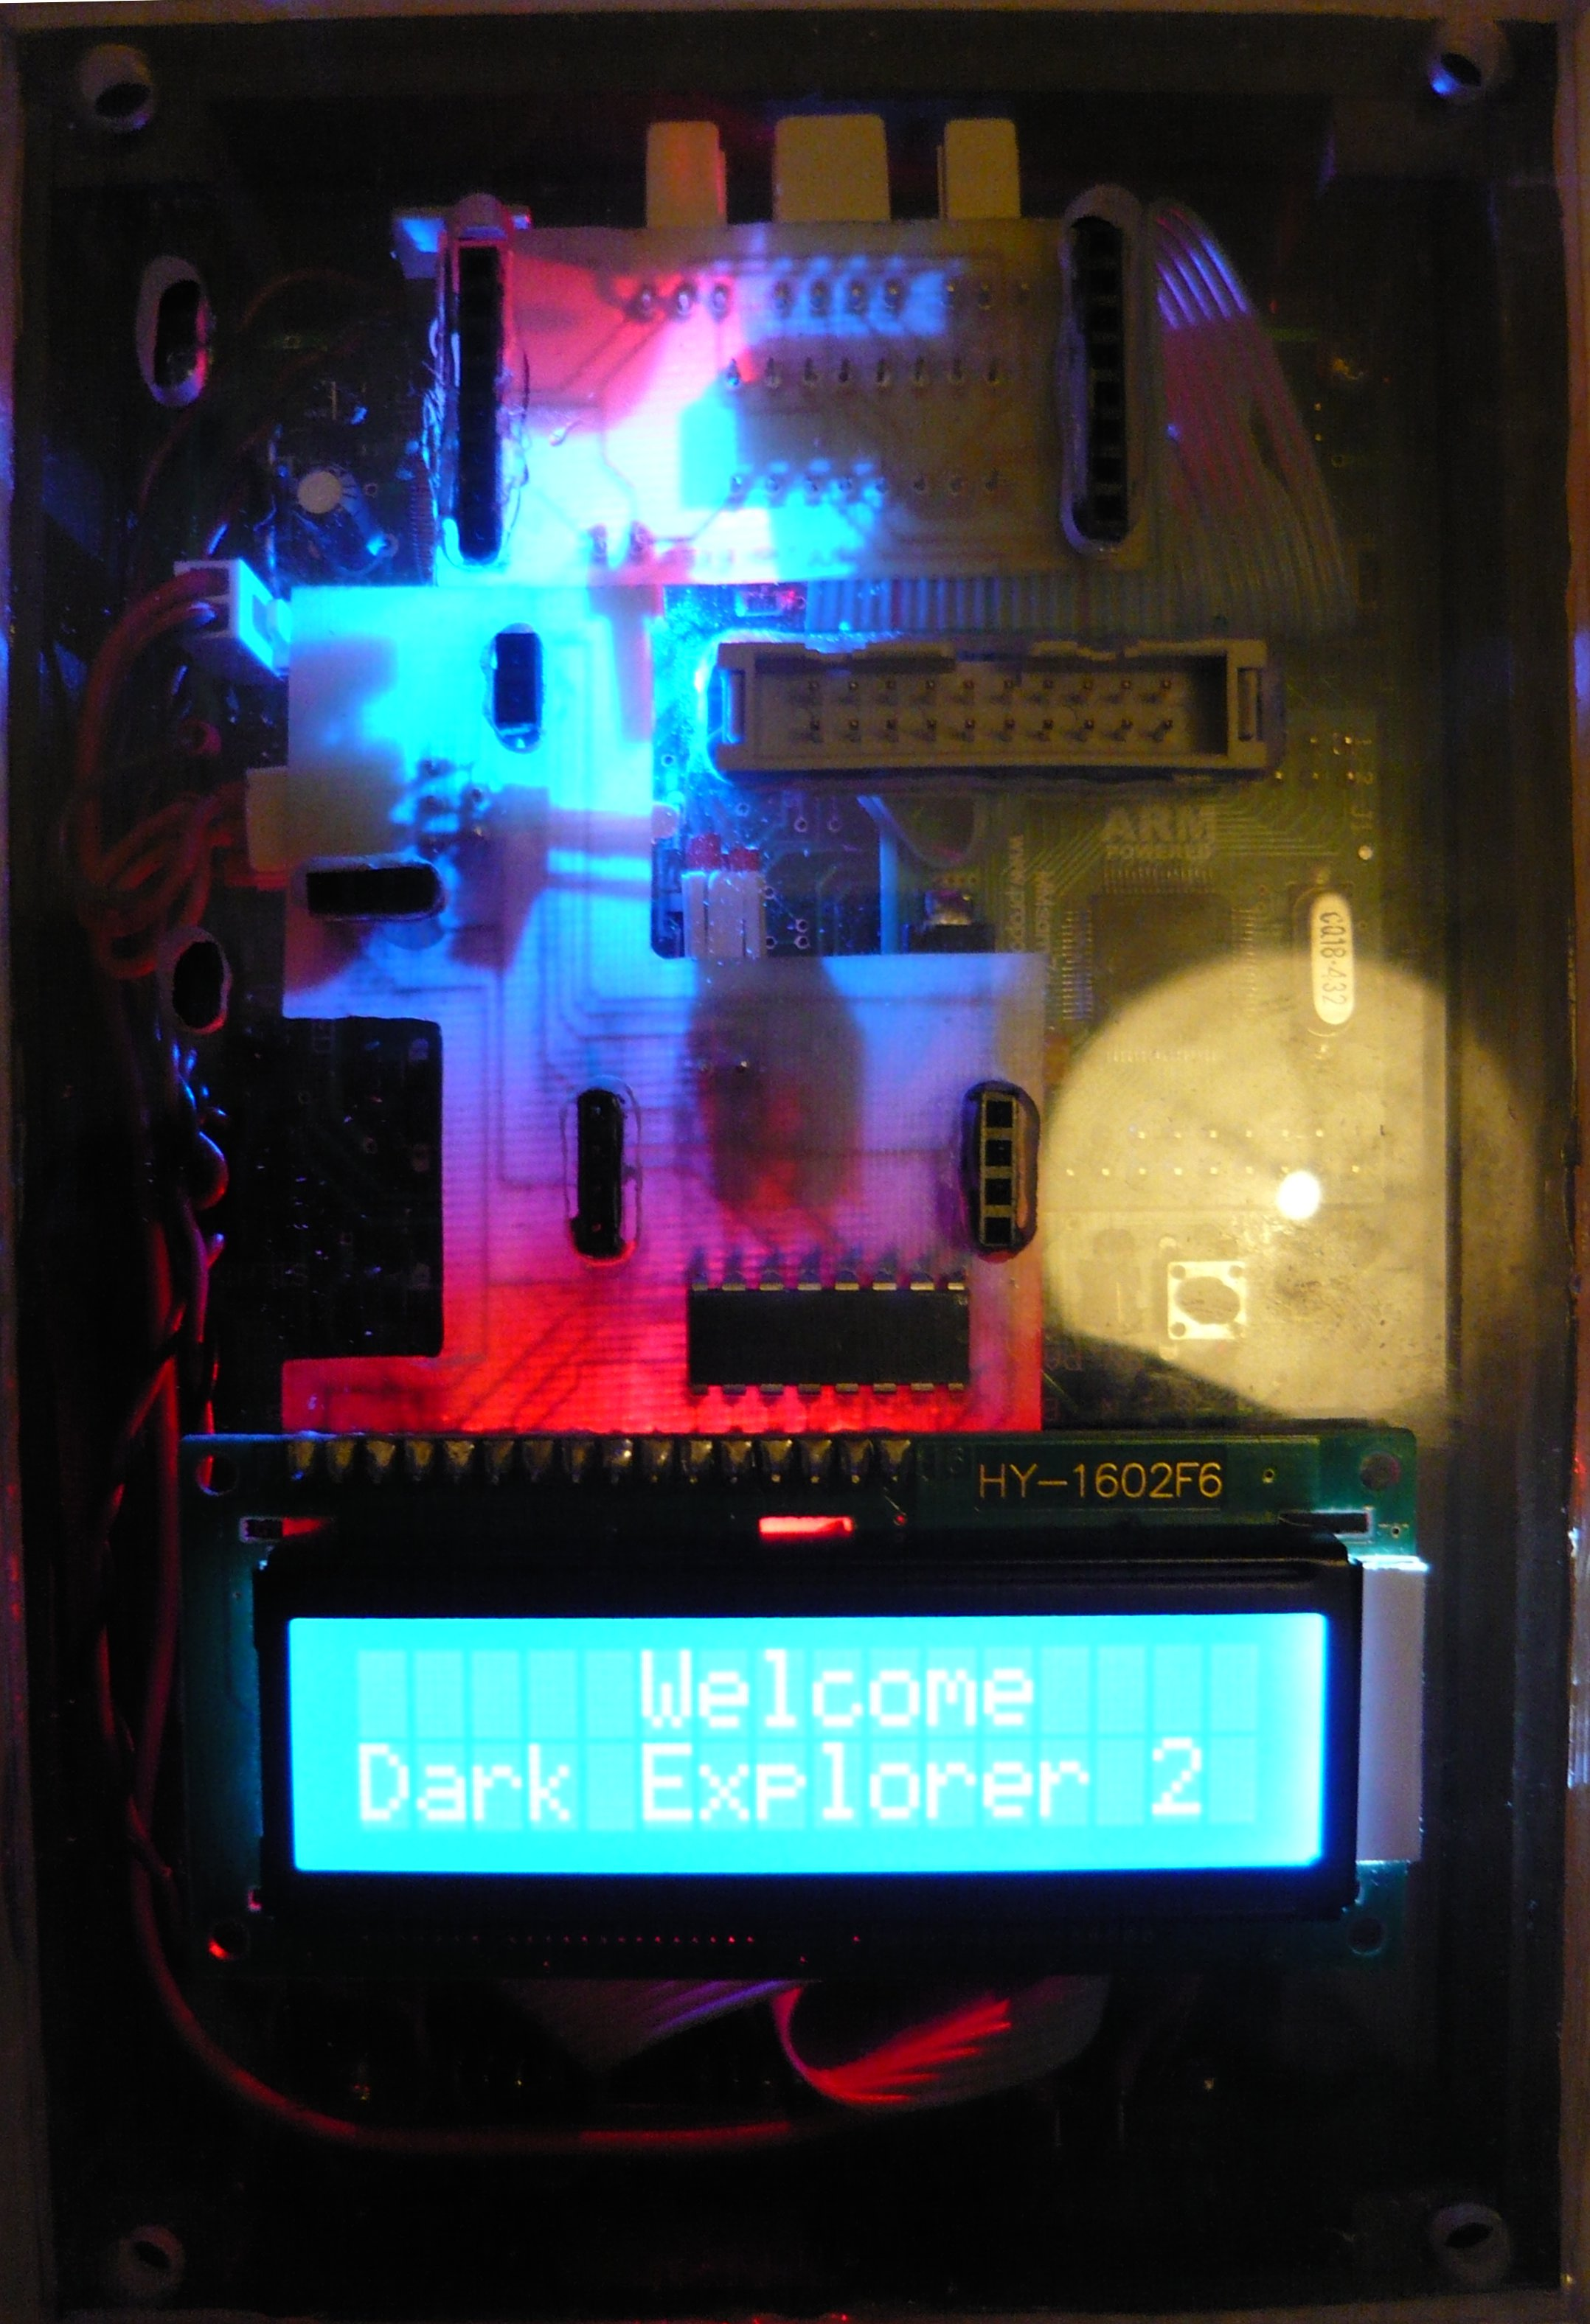
\includegraphics[height=75mm]{../images/ch04/lcd_welcome.jpg}
 \caption{Wyświetlacz LCD z komunikatem powitalnym}
 \label{fig:LCD}
\end{figure}

W celu wykorzystania wyświetlacza LCD konieczne było zastosowanie jakiegoś
sposobu na redukcję wejść oraz wyjść wykorzystywanych przez to urządzenie. W
konfiguracji podstawowej Dark Explorer udostępniał jedynie pięć złącz
GPIO\footnote{GPIO -- General Purpose Input/Output, złącza wejścia wyjścia
ogólnego przeznaczenia} natomiast sam wyświetlacz potrzebuje takich złącz sześć.
Z pomocą przyszedł tutaj 8-bitowy ekspander GPIO z interfejsem
$I^{2}C$\footnote{$I^{2}C$ -- szeregowa dwukierunkowa magistrala służąca do
przesyłania danych w urządzeniach elektronicznych}. Wykorzystany element to
PCF8574 firmy Philips. Układ ten posiada ośmio bitowy rejestr w którym
przechowuje słowo odebrane poprzez interfejs $I^{2}C$. Każdy bit tego rejestru
jest odzwierciedlany jako stan wysoki lub niski na odpowiednich wyjściach GPIO. W
taki sposób możliwe jest sterowanie wyświetlaczem LCD. Wykorzystując ten pomysł
można znacząco rozszerzyć ilość portów GPIO na robocie i sterować dowolnymi
urządzeniami.

\begin{figure}[!ht]
 \centering
 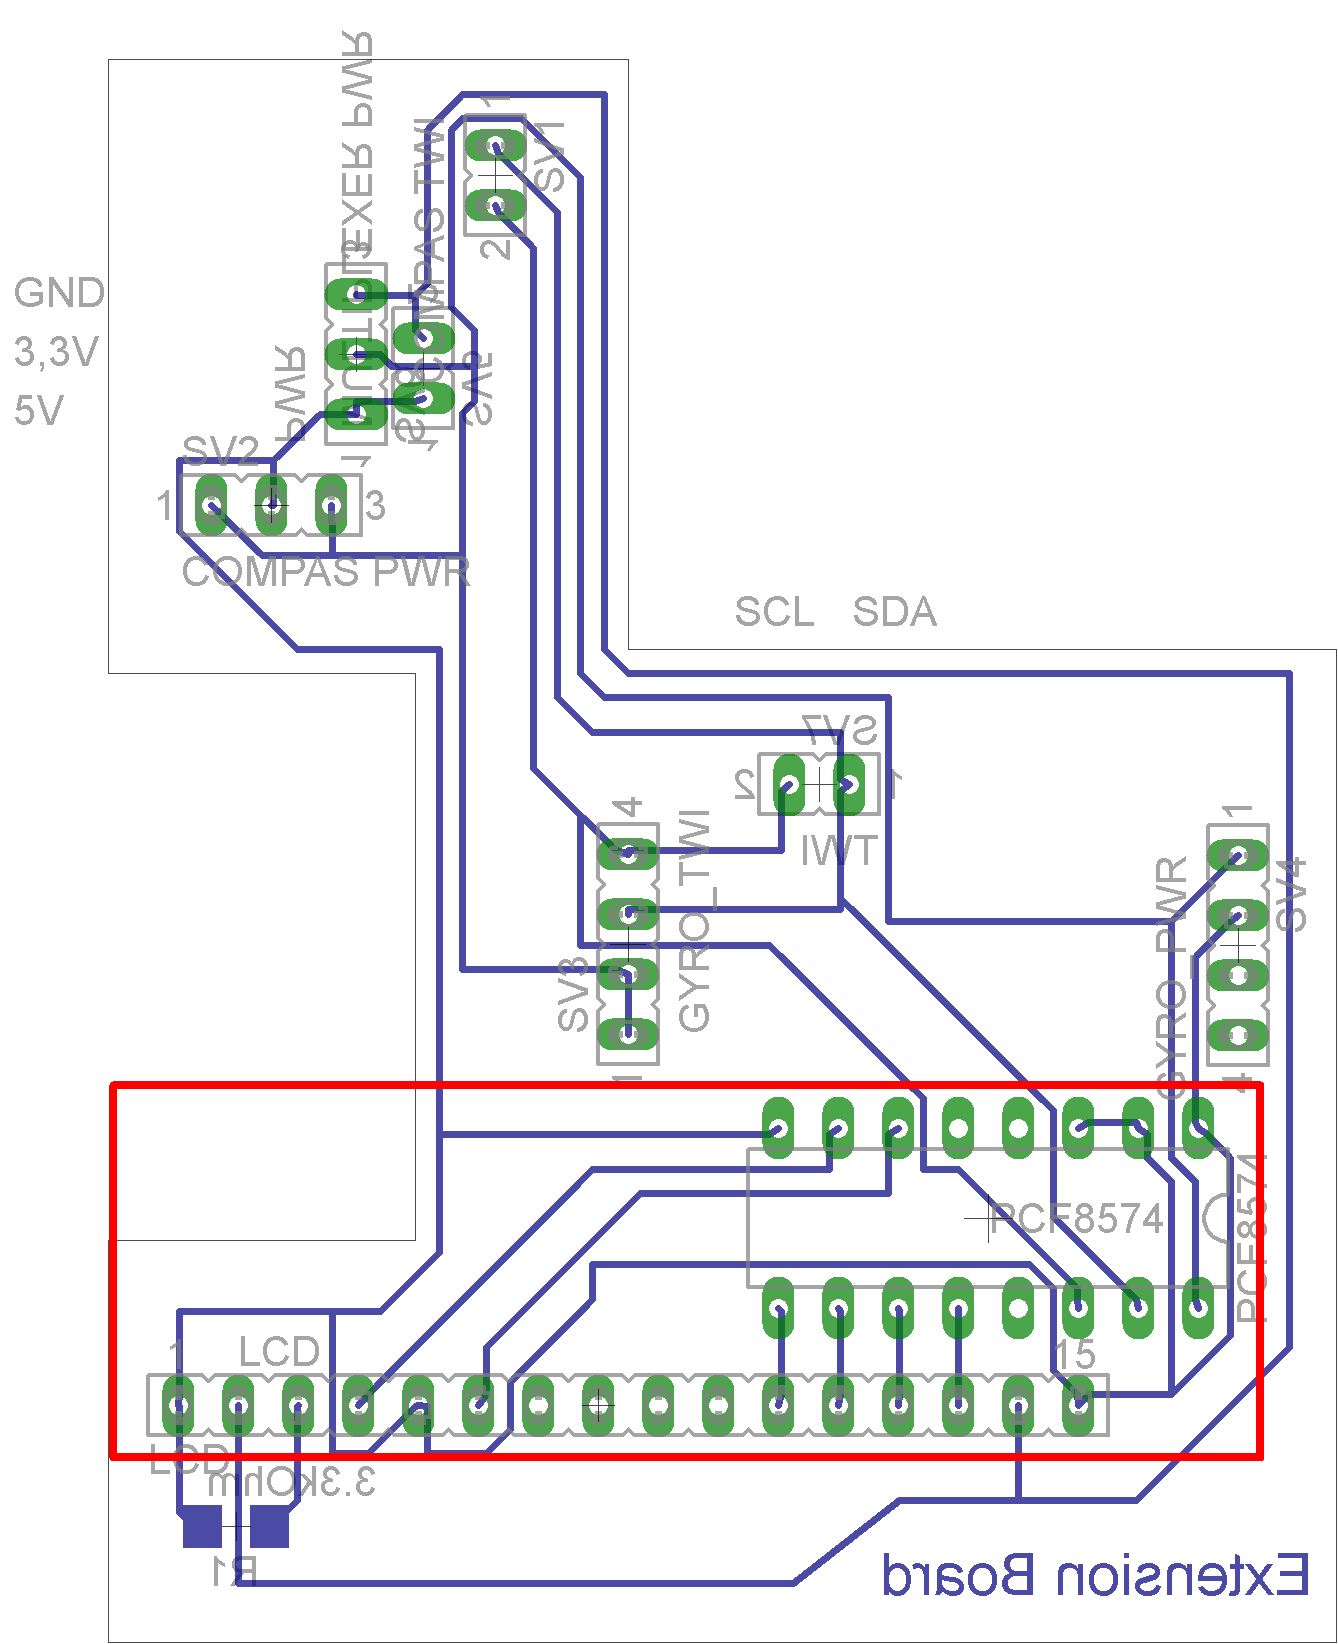
\includegraphics[height=75mm]{../images/ch04/extension_board-LCD.png}
 \caption{Płyta rozszerzeń z zaznaczonymi elementami odpowiedzialnymi za obsługę wyświetlacza LCD}
 \label{fig:ExBoardWithLCD}
\end{figure}

Wyświetlacz został zakupiony jako moduł z wtykiem 16 pinowym. Można go podłączyć
do gniazda LCD na płycie rozszerzeń Dark Explorera.


\chapter{Rozwój systemu wbudowanego}
\section{Protokół komunikacji bluetooth}
\label{sec:ch05_s01_comm}
Robot Dark Explorer komunikuje się z otaczającym go światem przy użyciu
technologii Bluetooth. Zaimplementowany w pierwotnej wersji oprogramowania
robota protokół komunikacji bazuje na ramce składającej się z 8 bitów nagłówka oraz 8 bitów
danych. Za pomocą informacji zawartych w nagłówku robot rozpoznaje
rodzaj akcji którą należy podjąć, natomiast po odczytaniu danych z kolejnego
przesłanego bajtu urządzenie jest w stanie uruchomić odpowiedni wariant metody
zdefiniowanej w nagłówku przesłanej ramki. Jeżeli wysłane polecenie wymusza
odesłanie danych zwrotnych są one transmitowane przez robota w~postaci czystego
strumienia bajtów bez żadnych dodatkowych metadanych.

\begin{figure}[h!]
 \centering
 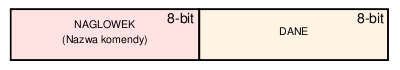
\includegraphics[height=18mm]{../images/ch05/old_req_schema.png}
 \caption{Schemat ramki komunikacyjnej w pierwotnej wersji robota}
 \label{fig:OldCommFrame}
\end{figure}

Zaprezentowane tutaj podejście jest bardzo wydajne i nie ogranicza efektywnej
przepustowości łącza poprzez konieczność przesyłania dodatkowych danych
związanych z obsługą protokołu komunikacji. Nie mniej jednak tego rodzaju
komunikacja wymaga, od programisty tworzącego aplikacje klienckie, głębokiej
znajomości sposobu realizacji poszczególnych poleceń, tak aby mógł on
synchronizować komunikację zarówno pod względem czasowy jak i logicznym. Ma to
szczególne znaczenie w przypadku wykonywania poleceń w sposób sekwencyjny gdzie
aplikacja klienta powinna oczekiwać na zakończenie wykonania poprzedniego
polecenia, jak ma to miejsce np. podczas pobierania obrazu z kamery. Kolejną
znaczącą niedogodnością jest fakt, iż bardzo często nawet najdrobniejsze zmiany w
oprogramowaniu robota wymuszają wprowadzanie zmian w aplikacji klienta pomimo
tego, że sposób wymiany komunikatów pozostał niezmieniony. Swego rodzaju
kłopotliwym problemem było również interpretowanie odpowiedzi przychodzących z
robota, gdyż aplikacja klienta musiała przechowywać informację na temat rodzaju i
formatu odpowiedzi która została odebrana w wyniku wykonania akcji. Co więcej
dotychczasowy sposób wymiany danych nie gwarantował również mechanizmów
wykrywania i zapobiegania błędom transmisji na poziomie aplikacji.

Zastosowana do wymiany danych technologia bluetooth posiada szereg standardowych
protokołów komunikacyjnych działających w ramach różnych warstw modelu
referencyjnego OSI. Niestety protokoły dostępne w warstwie aplikacji ograniczają
się jedynie do wymiany danych na temat kontaktów i synchronizacji danych
kalendarzowych, a~co~za~tym idzie nie nadają się do rozwiązania problemów
zdalnego sterowania urządzeń. Pełna~lista protokołów dostępnych w ramach
technologii bluetooth widoczna jest na rysunku \ref{fig:BtStack}. Niezmiernie
ważne jest aby przy projektowaniu schematu komunikacji w warstwie aplikacji, tak
dobrać protokół warstwy niższej aby realizował on jak najwięcej wymagań
postawionych przed systemem komunikacji.

\begin{figure}[h!]
 \centering 
 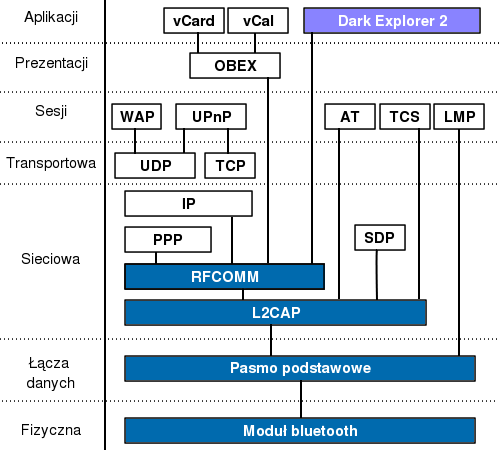
\includegraphics[height=100mm]{../images/ch05/btstack.png}
 \caption{Diagram protokołów bluetooth z podziałem na warstwy}
 \label{fig:BtStack}
\end{figure}

Aby zaadresować wszystkie napotkane w czasie rozwoju robota problemy konieczne
okazało się zaprojektowanie i zaimplementowanie nowego protokołu warstwy
aplikacji który ułatwiłby tworzenie oprogramowania współpracującego z rozbudowaną
wersją robota Dark Explorer. Konieczność taka wynika z faktu iż w warstwie
aplikacji nie istnieją protokoły które można bybyło zaadaptować na potrzeby
sterowania robotem.  Do implementacji protokołu komunikacji wykorzystany został
protokół RFCOMM\footnote{Radio Frequency Communication} gdyż gwarantuje on nam
korekcję błędów na poziomie pakietów. Wszystkie powiązane z nim protokoły
niższego poziomu zostały oznaczone kolorem na rysunku \ref{fig:BtStack}. Projekt
protokołu komunikacji bazuje na 16 bitowych ramkach bazowych. Każdy przesyłany
komunikat musi posiadać 16 nagłówek w odpowiednim formacie który pozwoli na jego
poprawne zinterpretowanie i przetworzenie. Komunikaty w niedozwolonym formacie
lub zawierające nieprawidłowe dane będą przez robota ignorowane.

W ramach opracowanego standardu wyróżnić można dwa rodzaje ramek. Do pierwszej grupy
zaliczyć można ramki żądań wysyłane przez urządzenia zewnętrzne w celu zlecenia
robotowi wykonania manewru lub rozpoczęcia kolejnych etapów bardziej złożonej
procedury. Diagram przedstawiający strukturę funkcjonalną ramki żądania widoczny
jest na rysunku \ref{fig:RfcommReqFrame}.

\begin{figure}[h!] 
 \centering
 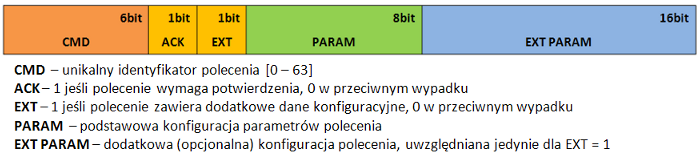
\includegraphics[width=\textwidth]{../images/ch05/req_schema2.png}
 \caption{Schemat funkcjonalny ramki komunikacyjnej z żądaniem}
 \label{fig:RfcommReqFrame}
\end{figure}

Pierwsze 6 bitów zostało zarezerwowane na unikalny identyfikator polecenia które
robot ma wykonać. Pozwala to na zdefiniowanie 64 niezależnych funkcjonalnie
komend w ramach których, w wersji podstawowej, możliwe jest uruchomienie 256
niezależnych wariantów polecenia. W przypadku wykorzystania wersji rozszerzonej
nagłówka programista ma do dyspozycji 24 bity które może przeznaczyć na dane
polecenia i identyfikator wariantu komendy w proporcjach odpowiadających
wymaganiom programisty. Kolejny bit nagłówka przeznaczony został na flagę potwierdzenia.
Umieszczenie 1 na wspomnianym bicie spowoduje iż robot po zakończeniu
wykonywania żądania prześle ramkę potwierdzającą ze statusem wykonania akcji.
Ułatwia to programiście wykonywanie czynności sekwencyjnych takich jak np. wykonanie
zdjęcia za pomocą kamery i przesłanie go do aplikacji klienta. Ósmy bit nagłówka
zarezerwowany został na flagę z informacją o użyciu rozszerzonej wersji
nagłówka. Wymuszenie 1 na tym bicie spowoduje, że robot będzie oczekiwał na
dodatkowe 16 bitów danych żądania które mogą zostać wykorzystane do przesłania
bardziej skomplikowanej konfiguracji wykonania polecenia. Kolejne osiem bitów
stanowi tzw. podstawową konfigurację polecenia, która może służyć jako
identyfikator przy uruchamianiu odpowiedniego wariantu polecenia lub jako nośnik
danych potrzebnych do zrealizowania przesłanej komendy. W przypadku gdyby
rozmiar bufora konfiguracyjnego nie pozwalał na przechowanie wszystkich
wymaganych danych programista może wykorzystać dodatkowe 2 bajty konfiguracji
rozszerzonej.

Drugi rodzaj ramek stanowią powiadomienia informujące użytkownika o rezultacie 
wykonania przesłanej akcji lub aktualnym stanie robota. Podobnie jak w przypadku
ramki z żądaniem pierwsze 6 bitów zarezerwowane jest na unikalny identyfikator
polecenia dla którego przesyłana jest odpowiedź. Kolejny bit zawiera flagę
informującą o rezultacie zakończenia akcji. Prawidłowe zakończenie wykonania
polecenia sygnalizowane jest ustawieniem zera na wspomnianym bicie. Wystąpienie
błędu podczas realizacji polecenia lub przesłanie komendy w nieprawidłowym
formacie spowoduje ustawienie 1 na bicie STATE. W przypadku gdy ilość
danych do przesłania przekracza maksymalny dopuszczalny rozmiar
pojedynczej ramki możliwe jest podzielenie danych na fragmenty i przesłanie ich
za pomocą sekwencji komunikatów. Koniec sekwencji sygnalizowany jest za pomocą
bitu EOT\footnote{End of Transmission}. Dostępność tego rodzaju trybu pozwala
na szybką transmisję większych ilości danych bez konieczności wysyłania żądań dla poszczególnych fragmentów.

\begin{figure}[h!] 
 \centering
 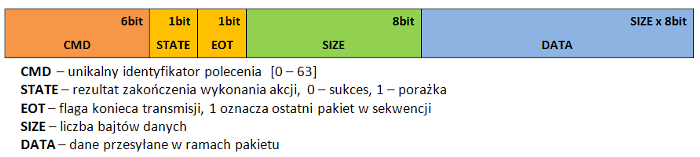
\includegraphics[width=\textwidth]{../images/ch05/resp_schema2.png}
 \caption{Schemat funkcjonalny ramki komunikacyjnej z odpowiedzią}
 \label{fig:RfcommRespFrame}
\end{figure}

Kolejne 8 bitów nagłówka odpowiedzi stanowi informacja o ilości bajtów
przesyłanych w sekcji danych ramki. Ogranicza to maksymalny rozmiar ramki przez
co transmisja danych nie powoduje licznych retransmisji które bardzo często
pojawiają się w przypadku transmisji większych ilości danych. Informacja o
szerokości pola danych ramki może również służyć jako suma kontrolna pozwalająca
na sprawdzenie czy wszystkie zadeklarowane dane zostały prawidłowo odebrane.
Pozwala to programiście tworzącemu oprogramowanie klienta na monitorowanie
transmisji i ewentualne reagowanie w przypadku pojawiania się problemów z
płynnością transmisji. 
\section{Algorytm rekonstrukcji ścieżki powrotnej}
\section{Lokalizacja twarzy na obrazie}
W ciągu ostatnich lat obserwuje się bardzo dynamiczny rozwój biometrii.
Aplikacje analizujące biometryczne cechy użytkowników znalazły swoje
zastosowanie miedzy innymi w systemach zabezpieczeń i monitoringu, robotyce,
komputerach przenośnych, aparatach i kamerach cyfrowych czy nawet w nowoczesnych
telefonach komórkowych. Pośród szeregu cech które mogą zostać poddane analizie
szczególnym zainteresowaniem cieszy się analiza ludzkiej twarzy. Systemy
posiadające możliwość zlokalizowania na obrazie twarzy od pewnego czasu
towarzyszą nam w życiu codziennym. Niemniej jednak większość istniejących
algorytmów pozwalających na rozwiązanie tego problemu jest
dosyć skomplikowana i ma bardzo konkretne wymagania zarówno co do platformy sprzętowej
jak i jakości obrazu który będzie poddawany analizie. Dlatego też stworzenie
implementacji dla platformy o bardzo ograniczonych zasobach obliczeniowych i
pamięciowych jest dużym wyzwaniem. Celem niniejszego rozdziału jest
przedstawienie podstawowych rodzajów algorytmów lokalizacji twarzy oraz
wskazanie ich wad i zalet. W dalszej części znajduje się szczegółowy opis
stworzonej implementacji algorytmu zastosowanego w realizowanej pracy magisterskiej.

\subsection{Algorytmy}
W ciągu ostatnich kliku lat rozwijanych było wiele różnych podejść poprawiających
wydajność procesu lokalizacji ludzkiej twarzy. Wśród nich można wyróżnić klika
głównych kategorii. Pierwszą z nich jest metoda opierająca się o bazę wiedzy.
Metoda ta pozwala na odszukiwanie niezmiennych cech twarzy nawet w bardzo
skomplikowanym otoczeniu, a przez to pozwala na ustalenie pozycji twarzy. Tego
typu podejście do problemu eliminuje problemy z uwzględnianiem ułożenia i pozycji
twarzy na obrazie. Statystyczny opis zależności pomiędzy poszczególnymi cechami
twarzy pozwala na stworzenie modelu który może posłużyć do zbudowania szablonu
twarzy dzięki któremu będziemy w stanie jednoznacznie stwierdzić czy na obrazie
widoczna jest twarz czy nie. Z takiego ujęcia problemu wywodzi się kolejna metoda
nazywana metodą porównywaniu szablonów (ang. template matching). Do stworzenia
wspomnianego szablonu twarzy mogą posłużyć takie parametry jak na przykład kolor
skóry, faktura twarzy czy też budowa twarzy. Wśród metod bazujących na
porównywaniu szablonów można wyróżnić dwa podejścia. Pierwsze z nich oparte jest
bezpośrednio na opisie cech twarzy i korzysta z opisu zależności pomiędzy
parametrami twarzy jako szablonu odszukując najbardziej pasujący do szablonu
fragment obrazu. Drugim podejściem jest stosowanie globalnego szablonu bazującego
na metrykach będących sumą poszczególnych cech za pomocą których jest opisany
szablon. Pierwsze podejście wymaga obrazu o stosunkowo dużej rozdzielczości ale
ponieważ nie bazuje ono na wszystkich punktach obrazu będzie obliczeniowo
bardziej wydajne niż podejście oparte o szablon globalny które może wymagać
przeszukania potencjalnie dużo większej grupy punktów obrazu wejściowego. Główną
wadą przestawionych do tej pory rozwiązań jest są ich dosyć wysokie wymagania.
Każdy z omówionych do tej pory algorytmów wymagał wykonywania kosztownych
obliczeń mających na celu poprzez dokonywanie przekształceń dopasowanie modelu
szablonu do zawartości obrazu wejściowego. Tak więc wykorzystanie tego typu
algorytmów wiąże się z koniecznością użycia stosunkowo mocnych jednostek
obliczeniowych co w przypadku platformy embeded mogłoby być problematyczne.\\
\\
Zupełnie innym podejściem do problemu lokalizacji twarzy jest wykorzystywanie
koloru skóry do odszukania fragmentów obrazu które potencjalnie mogłyby zwierać
twarz. Rozwiązania oparte o analizę kolorów można podzielić na dwie grupy w
pierwszej znajdują się rozwiązania bazujące na jednolitym kolorze tła w drugim
natomiast obraz wejściowy może zawierać tło o dowolnym stopniu złożoności.
Pierwsza z przedstawionych grup w znakomity sposób upraszcza problem odnalezienia
twarzy gdyż często usunięcie koloru tła z obrazu gwarantuje nam odnalezienie
wszystkich twarzy, zakładając, że obraz zawiera jedynie twarze. Jednakże jest to
podejście nakładające duże ograniczenia na warunki w jakich odbywa się akwizycja
obrazu. Dlatego też znacznie częściej porusza się problem lokalizacji twarzy w
oparciu o analizę kolorów z użyciem obrazów zawierających niejednokrotnie tło o
bardzo wysokim stopniu złożoności. Niemniej jednak wszystkie rozwiązania bazujące
jedynie o segmentację kolorów są w bardzo wysokim stopniu zależne od warunków w
jakim pobierany jest obraz wejściowy. Ze względu na zmieniające się warunki
otocznia może okazać się, że nasz algorytm nie uwzględnia wszystkich kolorów
skóry. Dodatkowym utrudnieniem jest pojawianie się grup pikseli które zostały
zakwalifikowane jako kolor skóry pomimo, że z twarzą nie mają nic wspólnego.
Problem ten jest szczególnie uciążliwy w przypadku obrazów o małych rozmiarach
gdyż trudno jest wtedy odróżnić twarz od szumów powstałych wskutek warunków
otocznia w który obraz był pobierany. Pomimo licznych swoich licznych wad
segmentacja kolorów jest jedną z najszybszych metod klasyfikacji obrazów pod
kątem obecności twarzy na obrazie. Co więcej narzut obliczeniowy na zastosowanie
klasyfikatora bazującego o model kolorów skóry jest proporcjonalny do rozmiarów
pobranego obrazu. Niestety jak się okazuje w praktyce sama segmentacja kolorów
jest niewystarczająca i wymaga
użycia dodatkowych metod w celu potwierdzenia odnalezienia twarzy. \\
\\
Kolejnym ciekawy rozwiązaniem pozwalającym na odszukanie twarzy na ruchomym
obrazie jest analiza ruchów twarzy. W tego typu rozwiązaniach obecność twarzy w
sekwencji wideo wykrywana jest na podstawie detekcji ruchów charakterystycznych
dla ludzkiej twarzy takich jak na przykład ruchy powiek. Mruganie jest ruchem na
tyle specyficznym, że wykrycie go pozwala jednoznacznie wnioskować o
lokalizacji twarzy na obrazie. Niestety przetwarzanie kilkudziesięciu klatek na sekundę o
rozmiarach pozwalających na zarejestrowanie ruchu powiek stawia dosyć wygórowane
wymagania związane nie tylko z algorytmem ale również z ilością danych jakie
klasyfikator musi przetworzyć w ciągu każdej sekundy nagrania. Istnieje jeszcze
wiele innych rozwiązań bazujących na bardzo wyszukanych metodach jak na przykład
użycie sieci neuronowych, jednakże ze względu na ich wygórowane wymagania
wykorzystanie jednego z nich dla platformy embeded z ograniczonymi zasobami
obliczeniowymi i pamięciowymi jest niezwykle trudne, a w niektórych przypadkach
niemal całkowicie niemożliwe.\\
\\
Algorytm implementowany w ramach pracy magisterskiej bazuje na podejściu opartym
o segmentacja kolorów. Aby wyeliminować niedoskonałości płynące z tego podejścia
algorytm w ostatnie fazie wykorzystuje informację o najprostszych cechach twarzy
w celu potwierdzenia obecności twarzy w obszarach zaklasyfikowanych jako kolor
skóry. Zastosowanie tego typu połączenia dwóch technik zaowocowało postaniem
algorytmu nie tylko szybkiego ale zarazem dającego stosunkowo dobre wyniki
analizy.

\subsection{Implementacja}
Implementacja modułu do lokalizacji twarzy na obrazie pobranym z kamery robota
została w całości oparta o algorytm zaproponowany przez Yao-Jiunn Chen, Yen-Chun
Lin w artykule zatytułowanym 'Simple Face-detection Algorithm Based on Minimum
Facial Features'. Autorzy do rozwiązania problemu używają obrazów o małej
rozdzielczości opisanych za pomocą modelu kolorów RGB. 

Zgodnie ze wskazówkami znalezionymi we wspomnianej publikacji, pierwszym krokiem
na drodze do zlokalizowania twarzy na obrazie jest akwizycja danych z kamery.
Przesłany z kamery obraz automatycznie jest poddawany podstawowej korekcji
mającej na celu dopasowanie balansu bieli oraz  dopasowanie ostrości. Tak
przygotowany obraz poddawany jest binaryzacji. Celem wspomnianego procesu jest
odnalezienie na obrazie obszarów będących w kolorze skóry oraz włosów. Zanim
jednak detekcja interesujących nas obszarów będzie możliwa konieczne jest
przeprowadzenie normalizacji modelu RGB. Zabieg tego typu pozwoli na usunięcie
zakłóceń wywołanych przez światła i cienie na obrazie pobranym z kamery robota.
Opisany proces normalizacji przeprowadzany jest poprzez pobranie wartości
poszczególnych kanałów RGB danego piksela obrazu, a następnie podzielenie tak
otrzymanej liczby przez sumę wartości wszystkich kanałów danego punktu.
Korzystając z takiego przepisu otrzymujemy następujący zestaw równań opisujący
normalizację każdego kanału z palety RGB.
\begin{eqnarray}
r = \frac{R}{R + G +B}\\
g = \frac{G}{R + G +B}\\
b = \frac{B}{R + G +B}
\end{eqnarray}
Na tak przygotowanym obrazie można już podjąć próbę odszukania punktów w kolorze
skóry i włosów. Do tego celu użyte zostały równania zaproponowane przez autorów
pracy źródłowej. Określają one rozkład kolorów ludzkiej skóry i włosów
wyznaczonych, jak twierdzą autorzy, w sposób eksperymentalny. Bazując na takich
założeniach ustalony został górny $F_1(r)$ i dolny $F_2(r)$ zakres kolorów w
jakich może znaleźć się ludzka skóra.
\begin{eqnarray}
F_1\left(r\right) = -1.376r^2 + 1.0743r + 0.2\\
F_2\left(r\right) = -0.776r^2 + 0.5601r + 0.18
\end{eqnarray}
Należy jednak zauważyć, że w zdefiniowanych w ten sposób równaniach mieści się
również kolor biały $r = 0.33 i g = 0.33$ dlatego też należy dodać następujący
warunek usuwający niechciany kolor z obszaru zainteresowania.
\begin{equation}
w = \left(r - 0.33\right)^2 + \left(g - 0.33\right)^2 > 0.001
\end{equation}
Po połączeniu obydwu równań otrzymujemy następujący układ równań opisujący
zakres kolorów jakie powinny reprezentować ludzką skórę. 
\begin{equation}
S = \left\{ 
\begin{array}{l l}
  1 & \quad \mbox{dla $g < F_1\left(r\right) \cap g > F_2\left(r\right) \cap w
  > 0.001$}\\ 0 & \quad \mbox{dla pozostałych}\\ \end{array} \right. 
  \label{skinEq1}
\end{equation}
Praktyczne doświadczenia z wykrywaniem obszarów skóry z zastosowaniem równania
\ref{skinEq1} wykazały iż niemal wszystkie obszary o kolorze skóry została
prawidłowo zaklasyfikowana. Znakomita większość pikseli nie stanowiących koloru
skóry została zastąpiona kolorem czarnym. Niemniej jednak wiele pikseli o
kolorze niebieski, żółtym i szarym również została błędnie sklasyfikowana. Aby
wyeliminować tego rodzaju efekt należy wykorzystać kryteria klasyfikacji oparte
o przestrzeń kolorów HSI. Poniżej przdstawiono zależność pomiędzy modelem RGB a
HSI.
\begin{equation}
\begin{array}{l}
\phi = cos^{-1}\left\{ \frac{0.5[(R-G)+(R-B)]}{\sqrt{(R-G)^2 + (R-B)(G-B)}}
\right\}\\\\
\left\{
\begin{array}{l l}
H=\phi & \mbox{dla B }\leq G\\
H=360^{\circ}-\phi & \mbox{dla B} > G
\end{array}
\right.
\end{array}
\end{equation}
Po skorzystaniu z przestrzeni HSI otrzymujemy następujący przepis na kolor
skóry.
\begin{equation}
S = \left\{ 
\begin{array}{l l}
  1 & \quad \mbox{dla $g < F_1\left(r\right) \cap g > F_2\left(r\right) \cap w
  > 0.001 \cap (H > 240 \cup H \leq 20 )$}\\ 0 & \quad \mbox{dla pozostałych}\\
  \end{array} \right.
  \label{skinEq2}
\end{equation}
Przy tak zdefiniowanym klasyfikatorze dokonywana jest binaryzacja całego obrazu.
Po przeprowadzeniu binaryzacji przeprowadzana jest kwantyzacja obrazu za pomocą
próbki o rozmiarze i wysokości pięciu pikseli. Pozwala to zminiejszyć
rozdzielczość obrazu, a co za tym idzie wyeliminować pewne rodzaje szumu oraz
znacznie uprościć dalsze obliczenia. Wspomniany proces kwantyzacji polega na
przeliczeniu liczby pikseli w kolorze skóry i kolorze czarnym w ramach 25
pikseli pobranych jako próbka obrazu. A następnie na podstawie wartości progowej
podjęcie decyzji czy cała próbka zostanie oznaczona kolorem skóry czy kolorem
czarnym. W ramach implementacji wartość progu została ustalona na poziomie 12
pikseli, oznacza to, że wszystkie próbki zawierające więcej niż 12 pikseli
czarnych są w całości oznaczane jako obszar niezawierający skóry i na odwrót.

\newpage
\chapter*{Podsumowanie}
Celem pracy był rozwój platformy sprzętowej i programowej robota mobilnego wraz
z oprogramowaniem umożliwiającym zdalne sterowanie robotem. Charakter pracy
wymagał podzielenia procesu realizacji zadań na klika etapów z których najważniejsze
zamieszczone zostały poniżej.
\begin{itemize}
  \item zapoznanie się i analiza możliwości robota Dark Explorer,
  \item odszukanie narzędzi oraz przygotowanie środowiska do rozwoju systemu
  wbudowanego robota dla systemu Windows oraz Linux,
  \item wybór zestawu czujników dodatkowych pozwalających rozszerzyć
  funkcjonalność robota bez konieczności ingerencji w dotychczasowe rozwiązanie,
  \item wykonanie obudowy oraz elektroniki umożliwiających podłączenie czujników
  do wolnych portów robota, 
  \item stworzenie modułowego systemu wbudowanego umożliwiającego sterowanie
  robotem wraz z użyciem dodatkowych czujników
  \item zaprojektowanie i wykonanie bibliotek zewnętrznych umożliwiających
  swobodne tworzenie oprogramowania sterującego robotem dla urządzeń
  stacjonarnych i przenośnych,
  \item przygotowanie przykładowych aplikacji sterujących pozwalających na
  zaprezentowanie możliwości robota po rozbudowie
\end{itemize}
Rozbudowany w ramach pracy magisterskiej robot w pełni realizuje cele założone
przez temat pracy. Unowocześniona wersja nie tylko znacząco rozszerza
funkcjonalność swego poprzednika ale również dzięki poczynionym modyfikacjom w
oprogramowaniu i elektronice robota znacząco ułatwia dalszą jego rozbudowę.

Rozbudowana wersja robota została wyposażona w dodatkowe czujniki wśród których
znaleźć można: akcelerometr, żyroskop, magnetometr oraz dalmierze IR. Wszystkie
wspomniane sensory są wykorzystywane przez robota do rejestracji
oraz rekonstrukcji ścieżki powrotnej po której poruszał się operator trzymający
robota w ręku. Zaimplementowany algorytm odtwarzania ścieżki nie wymaga do swojego działania
żadnej zewnętrznej infrastruktury. Dodatkowym atutem jest fakt, iż robot
wykorzystuje czujniki nie tylko podczas nagrywania przebytej drogi, ale również
podczas jej odtwarzania. Gwarantuje to, że działanie algorytmu jest całkowicie
niezależne od wpływów środowiska zewnętrznego np. śliska powierzchnia. Mechanizm
rekonstrukcji ścieżki wymaga od użytkownika, aby po zakończeniu
nagrywania ścieżki robot był zwrócony w kierunku powrotnym. Mimo dołożonych
starań zaprojektowane rozwiązanie nie gwarantuje, że robot zawsze dotrze do
punktu startowego. Wynika to z braku informacji o długości kroku wykonanego
przez operatora. Długość kroku została przyjęta jako wartość stała wyznaczona w
sposób doświadczalny i nie zawsze musi odpowiadać stanowi faktycznemu.
Dodatkowym utrudnieniem są ruchy wykonywane przez użytkownika w
trakcie zapamiętywania trasy takie jak np. nieutrzymywanie czoła robota
równolegle do kierunku ruchu operatora. Powoduje to rejestrowanie błędnych
parametrów trasy, co skutkuje deformacją odtwarzanego toru ruchu robota podczas
powrotu. 

Rozbudowana została również warstwa oprogramownia robota. Zebrano i
usystematyzowano wiedzę i narzędzia potrzebne do tworzenia oprogramowania
uruchamianego na nowej wersji robota Dark Explorer. Dołożono wszelkich starań,
aby możliwe stało się tworzenie aplikacji klienckich nie tylko na urządzenia
stacjonarne, ale również mobilne, takie jak telefony komórkowe. Zaprojektowane
biblioteki programistyczne umożliwiają korzystanie z funkcji robota, bez
konieczności zagłębiania się w szczegóły jego działania. 

Podczas pracy nad robotem udało się pokonać szereg problemów związanych z
ograniczeniami narzuconymi przez pierwotną konfigurację sprzętową. Mała ilość
wejść oraz wyjść zarówno cyfrowych jak i analogowych, została roszerzona przy
pomocy odpowiednio ekspandera GPIO dla interfejsu $I^{2}C$ oraz multipleksera
analogowo--cyfrowego. Przy wykorzystaniu tej samej metody, możliwe jest
rozszerzanie wejść/wyjść robota w praktycznie nieograniczony sposób. Udało się
także otrzymać zdjęcia w maksymalnej rozdzielczości, oferowanej przez kamerę
wbudowaną w robocie. Umożliwia to wykorzystanie kamery do przeprowadzania
bardziej złożonej analizy obrazu, niż było to możliwe w przypadku poprzedniej
wersji robota. Podjęto próbę implementacji algorytmu wykrywającego twarz, który
jest uruchamiany bezpośrednio przez mikrokontroler wbudowany w robota. 

Kolejne etapy rozwoju robota mogłyby wiązać się z przyspieszeniem akwizycji oraz
transmisji obrazu z kamery. W przypadku transmisji konieczne byłoby
wykorzystanie innego interfejsu komunikacji z modułem bluetooth (np. USB) lub
całkowita wymiana tego modułu na inną technologie. Przyspieszenie akwizycji
obrazu może zostać zrealizowane za pomocą dedykowanego programowalnego układu
FPGA lub poprzez rozszerzenie dostępnej pamięci podręcznej mikrokontrolera.
Drugie podejście najprawdopodobniej będzie wiązało się z wymianą samego
mikrokontrolera. W celu polepszenia działania inercjalnego systemu
nawigacyjnego, istotne byłoby rozważenie wymiany obecnie używanego akcelerometru
na inny o lepszych parametrach oraz podjęcie próby wyznaczenia za jego pomocą
dystansu jaki przebył robot. Następnym elementem poprawiającym obecną
funkcjonalność robota, może być dołączenie do niego kolejnych czujników
odległości, co pozwoliłoby na lepsze omijanie przeszkód. 

\newpage 
\appendix
\chapter{Wytrawianie płytek układów elektronicznych}
\chapter{Kod źródłowy}
%\begin{lstlisting} \end{lstlisting}
%\lstinputlisting[language=Python]{source_filename.py}
\listoffigures
\listoftables


\newpage

\bibliography{bibliography}{}
\bibliographystyle{plainpl}

\newpage

\end{document}
